%\documentclass[12pt]{report}

\documentclass  [
  paper    = a4,
  BCOR     = 10mm,
  twoside, % oneside für einfache seiten
  openany,  % openright für freiseiten vor kapiteln
  %parskip=half, % skip half a line between paragraphs instead of indent
  headsepline, % Trennlinie auf jeder Seite oben
  bibliography=totoc,
  fontsize = 12pt,
  %fleqn,
  toc      = bibnumbered,
  %toc      = listofnumbered,
  numbers  = noendperiod,
  headings = normal,
  listof   = leveldown]
  {scrbook}

\setkomafont{disposition}{\normalcolor\bfseries}


%\usepackage[a4paper]{geometry}
\usepackage[utf8]{inputenc}
\usepackage{amsmath, amssymb, amsthm}
\usepackage{siunitx}
\usepackage{xspace}
\usepackage{cleveref}
\usepackage{graphicx}
\usepackage{multicol, multirow, makecell}
\usepackage{caption}
\usepackage{subcaption}
\usepackage{tikz-feynman}
\usepackage{url} 

\DeclareSIUnit{\GeV}{\giga\electronvolt}
\DeclareSIUnit{\TeV}{\tera\electronvolt}
\DeclareSIUnit{\fbinv}{\per\femto\barn}

\newcommand{\todo}[1]{\textcolor{red}{\textbf{TODO} #1}}

\newcommand{\citere}[1]{Ref.~\cite{#1}}

\newcommand{\wrapmath}[1]{\ensuremath{#1}\xspace}

\newcommand{\ttbar}{\wrapmath{\mathrm{t \bar{t}}}}
\newcommand{\pptt}{\wrapmath{\mathrm{p p} \to \ttbar}}
\newcommand{\mt}{\wrapmath{m_{\mathrm{t}}}}
\newcommand{\mtt}{\wrapmath{m_{\ttbar}}}
\newcommand{\chel}{\wrapmath{c_{\mathrm{hel}}}}
\newcommand{\chan}{\wrapmath{c_{\mathrm{han}}}}
\newcommand{\cost}{\wrapmath{\cos \theta^*}}

\newcommand{\ptmiss}{\wrapmath{p_T^{\mathrm{miss}}}}
\newcommand{\ptmissvec}{\wrapmath{{\vec{p}_T}^{\mathrm{miss}}}}

\newcommand{\Lint}{\wrapmath{L_{\mathrm{int}}}}

\newcommand{\pt}{\wrapmath{p_T}}
\newcommand{\abseta}{\wrapmath{|\eta|}}
\newcommand{\sigmatt}{\wrapmath{\sigma_{\ttbar}}}
\newcommand{\mll}{\wrapmath{m_{\ell\ell}}}
\newcommand{\Rinout}{\wrapmath{R_{\mathrm{in/out}}}}
\newcommand{\alphas}{\wrapmath{\alpha_S}}

\newcommand{\ljets}{\wrapmath{\ell\mathrm{+jets}}}
\newcommand{\emu}{\wrapmath{\mathrm{e\mu}}}
\newcommand{\ee}{\wrapmath{\mathrm{ee}}}
\newcommand{\mumu}{\wrapmath{\mathrm{\mu \mu}}}

\newcommand{\sqrtsRIII}{$\sqrt{s} = \SI{13.6}{\TeV}$}
\newcommand{\xsecpred}{\wrapmath{921\hspace{1pt}^{+29}_{-37}\unit{pb}}}

\newcommand{\powheg}{\textsc{Powheg}\xspace}
\newcommand{\powhegvtwo}{\textsc{Powheg v2}\xspace}
\newcommand{\powhegvres}{\textsc{Powheg vRES}\xspace}
\newcommand{\amcatnlo}{\textsc{MG5\_aMC@NLO}\xspace}
\newcommand{\madgraph}{\textsc{MadGraph 5}\xspace}
\newcommand{\pythia}{\textsc{Pythia}\xspace}
\newcommand{\hdamp}{\wrapmath{h_{\mathrm{damp}}}}

\newcommand{\bbfourl}{\texttt{bb4l}\xspace}
\newcommand{\hvq}{\texttt{hvq}\xspace}
\newcommand{\ST}{\texttt{ST\_wtch}\xspace}
\newcommand{\ttb}{\texttt{ttb\_NLO\_dec}\xspace}
\newcommand{\tttW}{\wrapmath{\mathrm{\ttbar/tW}}}
\newcommand{\tttWsum}{\wrapmath{\mathrm{\ttbar+tW}}}
\newcommand{\rivet}{\textsc{Rivet}\xspace}

\newcommand{\AH}{\wrapmath{\mathrm{A/H}}}
\newcommand{\mA}{\wrapmath{m_{\mathrm{A}}}}
\newcommand{\mH}{\wrapmath{m_{\mathrm{H}}}}
\newcommand{\mAH}{\wrapmath{m_{\mathrm{A/H}}}}
\newcommand{\wA}{\wrapmath{\Gamma_{\mathrm{A}}}}
\newcommand{\wH}{\wrapmath{\Gamma_{\mathrm{H}}}}
\newcommand{\wAH}{\wrapmath{\Gamma_{\mathrm{A/H}}}}
\newcommand{\gAtt}{\wrapmath{g_{\mathrm{A t \bar{t}}}}}
\newcommand{\gHtt}{\wrapmath{g_{\mathrm{H t \bar{t}}}}}

\newcommand{\etat}{\wrapmath{\mathrm{\eta_t}}}

\newcommand{\sqrtsRII}{$\sqrt{s} = \SI{13}{\TeV}$}
\newcommand{\lumiVIII}{\SI{59.9}{\fbinv}}
\newcommand{\lumiVII}{\SI{41.5}{\fbinv}}
\newcommand{\lumiVI}{\SI{36.3}{\fbinv}}
\newcommand{\lumiVIpost}{\SI{16.8}{\fbinv}}
\newcommand{\lumiVIpre}{\SI{19.5}{\fbinv}}

\makeatletter
\g@addto@macro\bfseries{\boldmath}
\makeatother

\title{Measurement of the inclusive \ttbar production cross section and search for additional scalars in \ttbar final states
%\\
%The \pptt process: Inclusive cross section measurement and search for additional (pseudo-)scalars
}
\author{Laurids Jeppe}
\date{October 2024}

\begin{document}

\maketitle

\newpage
\tableofcontents
\newpage

\chapter{Introduction}
\label{ch:intro}

% begin : purpose of HEP - understand fundamental secrets of nature
% want to find new physics - but where to look
% promising: the top quark. heaviest SM particle - large Yukawa coupling to Higgs, new Higgs sectors, bare quark
% top quark colored, heavy, unstable - challenging to model in SM
% understanding top quark crucial for sm & bsm
% this thesis: study different aspects of ttbar production
% done as part of CMS, LHC, yadda yadda

% Run 3 of LHC: startup after shutdown, different calibrations etc
% new COM energy, energy frontier
% Run 3 ttbar xs measurement: first result of run 3
% validate data after shutdown

% study on off-shell ttbar / tttW interference modeling
% bb4l: full off-shell matrix element
% validated in CMS, compared to other generators
% input for future ttbar precision measurements

% search for new states in ttbar spectrum, Run 2, full lumi
% BSM: heavy higgs bosons
% top quark decays before hadronizing: access to spin information
% excess is observed!! wow
% close to trheshold, pseudoscalar
% interpreted as ttbar bound state, first observation
% difficult to probe, difficult to model in QCD
% also: interpretation in terms of generic BSM pseudoscalars, scalars
% separately: interpretation as ALP - phenomenology study

% outline of the thesis

% cite all publications

\chapter{Theoretical framework}
\label{ch:theory}

This chapter gives an outline of the theoretical concepts and models used in this thesis. It is split into two parts: First, the Standard Model of elementary particle physics is discussed, with a heavy emphasis on the top quark. Secondly, several hypothesized extensions of the Standard Model, relevant for the searches presented in ??, are briefly introduced and compared.

\section{Standard Model}

% content:
% particles, interactions, alphaEW, alphas
% top quark: mass, width, lifetime; decay into Wb;
% Yukawa coupling to Higgs, spin analyzing power
% Higgs mechanism: Higgs doublet in the SM, symmetry breaking, result: massive scalar particle; mass, coupling to massive particles
% pp -> ttbar: production diagrams (tree level), production modes (gg / qq), decays: allhad, semilep, dilep; mtt spectrum (?); spin states of ttbar
% spin density matrix: decomposition into polarizations and correlations, linear observables; cite new measurements
% nonperturbative: resummations close to the threshold, Couloumb resummation --> sorta bound state; comparison with J/Psi and Upsilon (large top width), difficulty of modeling: singlet v octet, Fuks model: singlet only, effective model, hints for observation in entanglement paper

The Standard Model of elementary particle physics, often simply called the Standard Model or SM, is, at the time of writing, the most successful theory describing the fundamental particles making up our universe. It is the result of a steady progression of increasingly complex models, starting with the introduction of quantum mechanics in the early 20th century and ending - for now - with the discovery of the Higgs boson at the LHC in 2012. The model has been extensively tested at many different experiments, most importantly the large collider experiments like LEP, the Tevatron, and the LHC. So far, it has survived all these tests with excellence.

\begin{figure}[ht]
    \centering
    \includegraphics[width=0.9 \textwidth]{figures/smsketch_colors.pdf}
    \caption{Schematic depiction of the particle content of the Standard Model, showing the seventeen fundamental particles, split into six quarks, six leptons, four gauge bosons, and the Higgs boson. The masses, electromagnetic charges, and spin of the particles is given next to the labels. Mass information is taken from \citere{PDG:2022pth}.}
    \label{fig:theory:sm}
\end{figure}

The SM is formulated as a relativistic quantum field theory (QFT). That is, its most fundamental objects are fields acting on four-dimensional spacetime which, after a quantization procedure, yield physically observable particles as fundamental excitations. By the usual counting scheme, there exist seventeen different such fields, which can be classified into different groups. The first group consists of the twelve fermions, which have spin $\frac{1}{2}$ and make up all visible matter. They are further split into the leptons, consisting of three electrically charged leptons - electron, muon, and tau lepton - and three corresponding electrically neutral neutrinos, as well as the quarks, of which there are six different flavors, called up, down, strange, charm, bottom, and top. The quarks have fractional electric charge, and in addition carry color charge as their defining property. Of note is that the fermions are also split into three generations, with each generation consisting of a charged lepton, a neutrino, and two quarks. The only fundamental differences between the particles of different generations are their masses, though the resulting physically observable properties, such as the lifetime, might be dramatically different.

The second group of particles are the bosons, which have integer spin. Here, the four gauge bosons with spin 1 act as the force carriers of the four fundamental interactions described by the SM: the photon, for the electromagnetic interaction with coupling strength $\alpha_{\mathrm{elm}}$; the W and Z bosons, for the weak interaction with coupling strength $\alpha_W$; and the gluon, for the strong interaction with coupling strength $\alpha_S$. At high enough energies, the electromagnetic and weak interaction unify into the electroweak interaction (coupling strength $\alpha_{\mathrm{EW}}$). The last and final particle is the Higgs boson, which has spin 0. Its most important role in the SM is to give mass to the fermions, as well as the W and Z bosons, through the so-called Higgs mechanism, which is briefly outlined in ??.

\subsection{Top quark}

All results presented as part of this thesis focus on one particular fundamental particle: the top quark. As such, it will be described in further detail in this section.

The top quark was first discovered in ?? at the Tevatron by the CDF and D0 experiments (refs). With a rest mass of $m_t = \SI{172.5}{\GeV}$, the top quark is the most massive known fundamental particle, and as a result it has unique properties compared to the other quarks: Its extremely short lifetime of $\approx \SI{5e25}{\s}$ is lower than the typical time needed for a quark to hadronize under the strong interaction, making it the only bare quark - that is, the only quark which,  via its decay products, is observable outside of hadrons. Among others, a consequence of this is that it fully preserves spin information during its decay, while such information is typically lost for other quarks during hadronization. More details on this are found in \cref{sec:theory:spindensity}.

A second extraordinary property of the top quark that follows from its high mass is its large Yukawa coupling to the SM Higgs boson, which is of order one. As a result, the Higgs boson couples preferentially to the top quark of all SM particles, and the study of both the SM Higgs boson and hypothetical additional Higgs bosons (see \cref{sec:theory:bsm}) is tightly connected to the top quark. 

In the SM, the top quark decays to a bottom quark and a W boson with a branching ratio (BR) of almost 100\% (to the degree that all other decays are commonly neglected). The W boson, in turn, can decay either to a charged lepton (e, $\mu$ or $\tau$) and the corresponding neutrino with a BR of $\sim 32.6\%$, or to a pair of quarks (one up- and one down-type) with a BR of $\sim 67.4\%$. This results in different final states for top production processes, which are discussed more in \cref{sec:theory:ttbar}.

\subsection{Higgs mechanism}

The Higgs boson is the most recently discovered particle of the SM. Its existence was confirmed in 2012 at the LHC by the ATLAS and CMS collaborations (refs), firmly establishing the SM in its current form as the accepted description of elementary particle physics. While this work does not focus on the SM Higgs boson as it does on the top quark, a short discussion of its role in the SM - the so-called Higgs mechanism - is relevant for possible SM extensions to additional Higgs bosons, which are searched for in \cref{ch:ah,ch:alps}.

In the SM Lagrangian, the Higgs boson appears as a complex doublet $\phi$ in the form

\begin{equation}
    \mathcal{L}_{\mathrm{SM}} \subset \left(D_\mu \phi\right)^\dagger D^\mu \phi + V(\phi)
\end{equation}

\noindent where $D_\mu$ is the covariant derivative, containing the minimal coupling to the gauge fields, and the Higgs potential $V(\phi)$ is 

\begin{equation}
    V(\phi) = \mu^2 \phi^\dagger \phi - \lambda (\phi^\dagger \phi)^2 .
\end{equation}

Here, $\mu^2$ and $\lambda$ are free parameters of the model. If both parameters are positive, this potential (known as the "Mexican hat potential") has a minimum at a non-zero value of

\begin{equation}
    | \phi | = \frac{\mu}{\sqrt{2 \lambda}} \equiv \frac{v}{\sqrt{2}}
\end{equation}

\noindent with the vacuum expectation value $v = \mu / \sqrt{\lambda}$. On the other hand, the minimum - corresponding to the vacuum state - is degenerate with respect to the three phases (i.e. the $SU(2)$ symmetry) of the complex doublet.

In the Higgs mechanism, this symmetry is now spontaneously broken in the transition from the high-energy state of the early universe (where the minimum is at $|\phi| = 0$) to the low-energy state observed today. The physical particles after symmetry breaking are then described by fluctuations around the new vaccum state. If the Higgs field were to be considered on its own, this would lead to one massive (corresponding to fluctuations in the $|\phi|$ direction) and three massless degrees of freedom (corresponding to the phases).

However, the interaction with the electroweak gauge fields encoded within $D_\mu$ leads to the massless degrees of freedom being absorbed into the gauge fields (\todo{ref}). This turns three of the four massless spin-1 gauge fields of the electroweak Lagrangian (with two degrees of freedom each) into massive fields instead (which have an additional longitudinal polarization, and thus three degrees of freedom). These three massive gauge fields are identified with the W and Z bosons, while the remaining massless field is identified with the photon. Finally, the leftover massive degree of freedom from the Higgs doublet $\phi$ is identified with the spin-0 boson observed at the LHC.

The resulting masses of the Z, W and Higgs bosons can be predicted as a function of $\mu^2$, $\lambda$ and the electroweak couplings and thus used to test the Higgs mechanism. In addition to the electroweak bosons, the Higgs mechanism can also give masses to fermions (charged leptons and quarks) by including a Yukawa interaction term in the Lagrangian. This results in couplings between the SM Higgs boson and the different fermions that are proportional to the respective fermion mass, leading to the largest coupling to the top quark. In possible extensions of the SM, this proportionality might be modified, making Yukawa coupling measurements attractive as tests of the SM.

\section{The \pptt process}
\label{sec:theory:ttbar}

In proton-proton collisions at the LHC, the dominant production mode of top quarks is the production of a top-antitop quark pair (\ttbar). The different parts of this thesis all focus on this process in different ways, and so this chapter gives a detailed overview of relevant effects.

At LO in QCD, there are three diagrams (up to permutations of initial and final states) contributing to \ttbar production, which can be seen in \cref{fig:theory:ttbar}. They differ in their initial states: the first two diagrams are induced by gluon fusion, while the last one is induced by quark fusion (mostly from $\mathrm{u \bar{u}}$ and $\mathrm{d \bar{d}}$). The fraction of these is determined by the corresponding parton densities; at a center-of-mass energy of $\sqrt{s} \geq \SI{13}{\TeV}$, gluon fusion dominates with a fraction of roughly 90\%.

\begin{figure}[t]
    \centering
    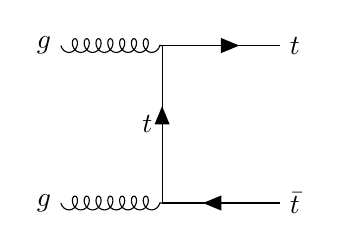
\begin{tikzpicture}[baseline=(current bounding box.center)]
      \begin{feynman}
        \vertex (i1) {\(g\)};
        \vertex [below=2.0 cm of i1] (i2) {\(g\)};
        \vertex [right=1.5 cm of i1] (a);
        \vertex [right=1.5 cm of i2] (b);
        \vertex [right=1.5 cm of a] (f1) {\(t\)};
        \vertex [right=1.5 cm of b] (f2) {\(\bar{t}\)};
        \diagram* {
          (i1) -- [gluon] (a),
          (i2) -- [gluon] (b),
          (f1) -- [anti fermion] (a) -- [anti fermion, edge label'=\(t\)] (b) -- [anti fermion] (f2)
        };
      \end{feynman}
    \end{tikzpicture}
    \hfill
    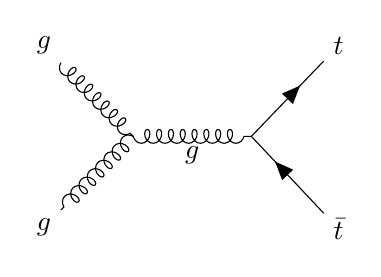
\begin{tikzpicture}[baseline=(current bounding box.center)]
      \begin{feynman}
        \vertex (a) ;
        \vertex [above left=1.3 cm of a] (i1) {\(g\)};
        \vertex [below left=1.3 cm of a] (i2) {\(g\)};
        \vertex [right=1.5 cm of a] (b);
        \vertex [above right=1.3 cm of b] (f1) {\(t\)};
        \vertex [below right=1.3 cm of b] (f2) {\(\bar{t}\)};
        \diagram* {
          (i1) -- [gluon] (a) -- [gluon] (i2),
          (a) -- [gluon, edge label'=\(g\)] (b),
          (f1) -- [anti fermion] (b) -- [anti fermion] (f2)
        };
      \end{feynman}
    \end{tikzpicture}
    \hfill
    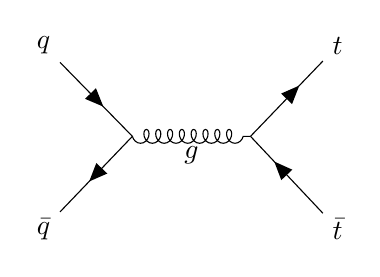
\begin{tikzpicture}[baseline=(current bounding box.center)]
      \begin{feynman}
        \vertex (a) ;
        \vertex [above left=1.3 cm of a] (i1) {\(q\)};
        \vertex [below left=1.3 cm of a] (i2) {\(\bar{q}\)};
        \vertex [right=1.5 cm of a] (b);
        \vertex [above right=1.3 cm of b] (f1) {\(t\)};
        \vertex [below right=1.3 cm of b] (f2) {\(\bar{t}\)};
        \diagram* {
          (i1) -- [fermion] (a) -- [fermion] (i2),
          (a) -- [gluon, edge label'=\(g\)] (b),
          (f1) -- [anti fermion] (b) -- [anti fermion] (f2)
        };
      \end{feynman}
    \end{tikzpicture}
    \caption{\textbf{Feynman diagrams for \pptt.} The three diagrams (up to permutations) that contribute to the \pptt process at LO in QCD.}
    \label{fig:theory:ttbar}
\end{figure}

At NLO in QCD, many more diagrams become relevant, including those induced by the fusion of one quark and one gluon, while radiating a real quark. Similarly, real emissions of gluons can take place in $gg$ or $q\bar{q}$ fusion diagrams. These effects change the kinematic properties of the produced top quarks, leading to NLO corrections for predicted distributions.

After production, both the top quark and antiquark in the \ttbar pair decay into a W boson and a b (anti)quark each. This leads to three different decay channels of the \ttbar pair depending on the decays of the two W bosons, which are classified according to their number of leptons: The dilepton channel, with final state $b \bar{b} \ell^+ \ell^- \nu \bar{\nu}$; the lepton+jets channel, with final state $b \bar{b} \ell \nu q \bar{q}$; and the all-hadronic channel, with final state $b \bar{b} q q \bar{q} \bar{q}$. Here, $q$ stands in for any light quark ($u$, $d$, $s$ or $c$).

The three channels differ greatly in their experimental challenges: The dilepton channel has the lowest branching ratio of $\sim 10.6\%$, which is further reduced to $\sim 5.1\%$ when excluding $\tau$ leptons due to then being experimentally hard to reconstruct. It also suffers from the fact that the two produced neutrinos escape the detector unobserved and are only measured as missing transverse momentum, losing both information in the forward direction as well as the ability to disentangle the two neutrinos. On the other hand, the final state of two opposite-sign charged leptons, two b jets, and missing transverse momentum does not have many other contributing processes in the SM, leading to very pure selections (particularly when the two leptons are an electron and a muon). The results in \cref{ch:ttxs,ch:bb4l,ch:ah,ch:alps} all make use of this channel prominently.

By contrast, the lepton+jets channel has a large BR of $\sim 43.9\%$ ($\sim 30.3\%$ when excluding $\tau$ leptons), leading to high data statistics, and easier interpretation of missing transverse momentum due to only one neutrino. However, it can suffer from contamination by W+jets and multijet QCD background (the latter with non-prompt or fake leptons), from issues with combinatorics (i.e. the assignment of experimentally measured jets to the decay products) and from hadronic jet uncertainties, which can be large. This decay channel is employed for the result in \cref{ch:ttxs} as well as in the combination in \cref{ch:ah}.

Finally, the all-hadronic channel, with a similar BR of $\sim 45.4\%$, is typically difficult to isolate from the background of QCD multijet production, and in addition suffers even more strongly from combinatorics and jet uncertainties then the lepton+jets channel. As a result, it is in most cases the least precise of the three channels, and is not studied further in this work.

\subsection{Spin density matrix}
\label{sec:theory:spindensity}

As fermions with spin $\frac{1}{2}$, top quarks have two possible spin states. As a result, the relative spins of the \ttbar system can be either aligned, leading to a total vector state with spin 1, or anti-aligned, leading to a scalar state with spin 0. In proton-proton collisions, a mix of both these states is produced, with the ratio depending on the production mode ($gg$, $q\bar{q}$ or $gq$) as well as the energy.

A way of quantifying the production of the different spin states, respective to an arbitrary spin basis, is the production spin density matrix $\mathbf{R}$, which (when averaged over initial spins and colors, and summed over final colors) can be written as

\begin{equation}
    \mathbf{R} = A \, \mathbb{1} \otimes \mathbb{1}
    + B_i^1 \, \sigma_i \otimes \mathbb{1}
    + B_i^2 \, \mathbb{1} \otimes \sigma_i
    + C_{ij} \, \sigma_i \otimes \sigma_j.
\end{equation}

Here, $\mathbb{1}$ is the two-dimensional identity matrix, $\sigma_i$ with $i=1,2,3$ are the Pauli matrices, and the first and second components of the tensor product refer to the spin of the top quark and antiquark, respectively. The scalar coefficient $A$ describes the overall amplitude (i.e. the cross section) of \ttbar production, the vectors $\vec{B}^1$ and $\vec{B}^2$ describe the polarization of the top quark and antiquark, and the matrix $\mathbf{C}$ describes the correlation between their spins. All of them are, in general, functions of the partonic center-of-mass energy and the scattering angle of the top quark relative to the incoming partons.

In practice, the spins of the top quarks can not be observed directly, and instead must be inferred from their decay products. The way the spin information is passed to the decay products is determined by the weak interaction, which is maximally parity-violating. In particular, for a leptonic decay $t \rightarrow b \ell^+ \nu$, 

% next: a) choice of basis - helicity basis by Bernreuther
% b) decay products - weak interaction (V-A), ??? try to understand this shit

\subsection{Non-perturbative effects}

\section{Beyond the Standard Model}
\label{sec:theory:bsm}

\subsection{Extended Higgs sector models}
\label{sec:theory:hext}

\subsection{Axion-Like Particles}

\chapter{Monte Carlo event generation}

\section{Monte Carlo method}

\section{Matrix Element generators}

\section{Parton showers and matching}


\chapter{Experimental methods}
\label{ch:methods}

\section{The Large Hadron Collider}

\section{The CMS experiment}

\section{Data reconstruction}
\label{sec:methods:reco}

\section{Statistical interpretation}

In experimental particle physics, results are typically extracted by comparing detector-level predictions, for example obtained using MC simulation, to the observed data for suitably chosen observables. The measured data here are neccesarily afflicted by statistical uncertainties, both due to the inherent randomness of quantum mechanics and the probabilistic behaviour of the detector. They should thus be seen as a sample drawn from a random distribution, and in order to extract underlying parameters of any model, statistical methods are required.

In this work, all statistical interpretation is performed in the framework of \textit{binned profile maximum likelihood fits}. This method follows the Frequentist approach of considering physical properties that should be extracted to be fixed, if unknown, quantities, which enter the random distribution of the observed data as parameters. In order to estimate the desired properties, the observed datapoints are sorted into orthogonal bins according to one or more sensitive observables, and each bin is treated as an independent counting experiment where the observed number of events is given by a Poissonian distribution. 

Denoting the set of physical properties to be estimated (the parameters of interest or POIs) collectively as $\vec{\mu}$, the likelihood of $\vec{\mu}$ for bin $i$, given that $N_i$ events were observed, is

\begin{equation}
    L_i (\vec{\mu}, \vec{\theta}) = \mathrm{Pois} \left(N_i | n_i (\vec{\mu}, \vec{\theta}) \right)
\end{equation}

Here, $\mathrm{Pois}$ refers to the Poissonion distribution, and $n_i (\vec{\mu}, \vec{\theta})$ is the mean expected number of events in bin $i$ as predicted by the 

\chapter{Measurement of the inclusive \ttbartitle cross section at \texorpdfstring{$\sqrt{s}$}{sqrt(s)} = 13.6 TeV}
\label{ch:ttxs}

%This chapter describes the measurement of the inclusive \ttbar production cross section at the LHC at the center-of-mass energy of \sqrtsRIII. First, a motivation and overview of the analysis design will be given. Then, object and cut definitions as well as several applied corrections will be explained in detail. Finally, the likelihood fit used to extract the cross section, including all uncertainties, is described and the result discussed.

\section{Introduction}

% motivation: new com energy, possible glimpse at new physics; new run, new calibrations, top physics requires most objects -> good check of performance

% method needs to be tuned for early measurement
% special mention: lepton sf -> can be estimated in situ
% do one fit with and one without

In July 2022, the LHC officially resumed collecting data after over three years of shutdown, thereby starting LHC Run~3. It did so at a new, unprecedented center-of-mass energy of \sqrtsRIII, inviting the experiments to measure physical observables at the new energy frontier.

One important such observable is the inclusive \ttbar production cross section. It is, in essence, the total rate of top quark pair production at the LHC, integrated over the kinematic distributions of the particles produced. As mentioned in \cref{ch:theory}, the top quark has a special place in the standard model as the heaviest known elementary particle, as well as the only colored particle that decays before hadronizing. 
It is thus important for many potential BSM scenarios, such as models with additional Higgs bosons, which might couple strongly to the top quark. 
As such, measurements of top quark-related observables at the highest possible energies are attractive tests of the SM. The inclusive \ttbar production cross section, as one of the simplest top quark observables, is well suited for a first measurement at the new center-of-mass energy.

Simultaneously, restarting such a large experiment as CMS after a three-year shutdown poses many experimental challenges. Due to the change in energy, as well as physical changes in the accelerator and detector, new calibrations as well as validations of some previous calibrations are required to ensure that the detector performance is understood. An early measurement of the inclusive \ttbar cross section is well suited to serve as such a cross-check: Because of the decay chain of the top quark, a top quark measurement involves many of the different objects reconstructed at CMS, which
%, as described in Ch. \ref{sec:methods:reco}, 
allows for a check of a wide landscape of calibrations.

The measurement described in this chapter was designed specifically with these motivations in mind, and as such exhibits several novel features. Firstly, it combines events from both the dilepton and \ljets decay channels of \ttbar, categorized by lepton flavor content, combining the higher statistics of the \ljets channel with the high purity of the \emu channel and allowing to constrain uncertainties on the lepton identification efficiency directly from the data. This is done using a simultaneous maximum likelihood fit to the event yields in the different categories, with experimental and theoretical uncertainties treated as nuisance parameters.

Secondly, the events are additionally categorized by their number of b-tagged jets, which similarly allows for an in-situ measurement of the b-tagging efficiencies. This averts needing to wait for external b-tagging calibrations, allowing for a measurement as early as possible.

The results of this work were first presented as a Physics Analysis Summary in September~2022~\cite{CMS:TOP-22-012-PAS}, only two months after the start of data taking, as the first public physics result of LHC Run~3. It was later published in \textit{JHEP} as \citere{CMS:TOP-22-012}, again representing the first published Run~3 result. A similar result by ATLAS was later published in \citere{ATLAS:2023slx}.

This chapter is structured as follows: In \cref{sec:ttxs:setup}, the used data sets, object definitions, and event selection criteria are described, followed by the derivation and application of needed corrections in \cref{sec:ttxs:corrections}, and the resulting data-MC agreement is shown in \cref{sec:ttxs:control}. The considered systematic uncertainties are listed in \cref{sec:ttxs:systematics}, and the fit results are presented in \cref{sec:ttxs:fitresults}. The chapter is concluded by a short summary and outlook in \cref{sec:ttxs:summary}.

\section{Data sets and event selection}
\label{sec:ttxs:setup}

In this section, the choice of data sets for experimental data and for simulation, as well as the choice of triggers, is described. Following that, the object and event selection procedure is outlined and several event categories to be used in the likelihood fit are defined. 

\subsection{Data sets}
\label{sec:ttxs:datasets}

\paragraph{Experimental data}
The measurement is performed on data recorded during the period between July 27\textsuperscript{th} and August 02\textsuperscript{nd} 2022, corresponding to an integrated luminosity of \lumiRIII. This amount of data is chosen as a balance between sensitivity and speed for the early measurement: It roughly corresponds to the point where the measurement precision is no longer primarily limited by the quantity of the data, while at the same time restricting to a data set where beam and detector conditions were stable and comparable to the data-taking in Run~2.

% TODO luminosity measurement

Both single-lepton and dilepton triggers were used to select events used in this measurement during detector operation, identifying leptons in the range of $\abseta < 2.5$. The \pt requirements of the triggers are summarized in Tab.~\ref{tab:ttxs:triggers}.

\begin{table}
    \centering
    \begin{tabular}{c|c}
        Trigger & Lepton requirement \\
        \hline
        \hline
        \ejets & e($\pt > 32$ GeV) \\
        \mujets & \textmu($\pt > 27$ GeV) \\
        \ee & e($\pt > 23$ GeV) and e($\pt > 12$ GeV) \\
        \mumu & \textmu($\pt > 17$ GeV) and \textmu($\pt > 8$ GeV) \\
        \emu & e($\pt > 23$ GeV) and \textmu($\pt > 8$ GeV)  or \\
        & e($\pt > 12$ GeV) and \textmu($\pt > 23$ GeV)
    \end{tabular}
    \caption{\textbf{Trigger definitions} as used for the \ttbar cross section measurement. The leptons are required to be isolated and in the pseudorapidity range  $\abseta < 2.5$.}
    \label{tab:ttxs:triggers}
\end{table}

\paragraph{Simulation}
To compare the data with predictions, Monte Carlo (MC) simulation is used to simulate both the \ttbar signal as well as most important background processes, specifically single-top quark production in the $t$-channel, associated tW production, Z+jets production, W+jets production, and diboson (WW, WZ and ZZ) production. The MC generator \textsc{Powheg v2}~\cite{Powheg:2004, Powheg:2007, Powheg:2010} is used to generate \ttbar, $t$-channel single-top, and tW events at next-to-leading order (NLO) in perturbative QCD, while the generators \textsc{MadGraph5\_aMC@NLO}~\cite{MG5aMCatNLO:2014} and \textsc{Pythia 8}~\cite{Pythia:2015} are used to generate Z+jets/W+jets and diboson events, respectively, at leading order (LO). For Z+jets and W+jets, up to four additional jets are included in the matrix element using the MLM matching scheme~\cite{Mangano:2006rw}. For $t$-channel single-top, \textsc{MadSpin} is used to simulate the top decay.

All of the generated events are interfaced to \textsc{Pythia 8} for parton showering and hadronization, and further processed in a full simulation of the CMS detector as described in \cref{ch:mc}. The proton structure in the matrix element calculation is described by the NNPDF3.1 parton distribution function (PDF) set at NNLO. Note that another background contribution, from QCD-produced multijet events with fake or non-prompt leptons, is not simulated, but estimated from data (see \cref{sec:ttxs:datadriven}).

Theoretical predictions, as well as the measured integrated luminosity, are used to normalize the cross sections of the signal and background samples as follows: The \ttbar signal, is normalized to a cross section of \xsecpred computed at NNLO+NNLL in QCD~\cite{Czakon:2011xx}, which is also used as a prediction for comparison with the SM. For the other backgrounds, the following orders in QCD and methods or programs are used: \textsc{MCFM}~\cite{Campbell:2020fhf} (NNLO) for single-top, \textsc{DYTurbo}~\cite{Camarda:2019zyx} (NNLO) for W+jets and Z+jets, \textsc{Matrix}~\cite{Grazzini:2017mhc} (NLO) for diboson, and an NNLO calculation from Ref. \cite{Kidonakis:2021vob} for tW.


\subsection{Object definition}
\label{sec:ttxs:objects}

\paragraph{Leptons}

Electrons or muons are considered for the analysis if they have $\pt > 10$ GeV and $\abseta < 2.4$. For electrons, the range $1.44 < \abseta < 1.57$, corresponding to the transition region between barrel and endcaps in the ECAL, is removed. Furthermore, additional identification criteria (ID) are applied to remove non-prompt or fake (i.e. wrongly reconstructed) leptons and enrich the selection with \ttbar events.

For electrons, the ``tight'' working point of the cut-based ID described in \citere{CMS:EGM-17-001} is applied, which includes information from both the details of the electromagnetic shower in the ECAL and the track, as well as the matching between the two. It also includes a requirement for the electron to be isolated from other particles such as hadrons, which is implemented in the form of the relative isolation variable \Irel. It is defined as the scalar \pt sum of all particles in a cone around the lepton in question, divided by the lepton \pt. Here, $\Delta R = \sqrt{(\Delta \eta)^2 + (\Delta \varphi)^2} < 0.3$ is used for the radius of the cone. Additional corrections accounting for pileup particles are applied.

For muons, a similar cut-based ID is used as described in \citere{CMS:MUO-16-001}, also at the tight working point. Here, criteria on the compatibility of tracks in the inner tracker, the muon detectors and the reconstructed primary vertex are employed. Again, a cut on \Irel is used, defined equivalently but with a cone size of $\Delta R < 0.4$.

\paragraph{Jets}

The anti-$k_T$ algorithm~\cite{Cacciari:2008gp} is used to cluster reconstructed particles into jets with a distance parameter of 0.4. In order for a jet to be considered, it is required to have $\pt > 30$ GeV and $\abseta < 2.4$, and jets overlapping with any considered leptons (i.e. fulfilling the above criteria) are removed. %Again, additional ID criteria, based on the fractions of \pt originating from neutral hadron, charged hadron and electromagnetic jet constituents, are used to reject 

\paragraph{Tagging of b jets}

A special role is played by jets originating from the showering and hadronization of b quarks. Naively, two such jets are expected per \ttbar event from the two top decays, although in practice one or both jets may fall out of acceptance of the detector or otherwise not be identified. Furthermore, additional b quarks may be produced by radiation at higher orders in QCD. Correctly tagging these jets as such can greatly improve signal purity by cutting away backgrounds such as Z+jets, W+jets and QCD multijet events.

Here, the \textsc{DeepJet} algorithm~\cite{DeepJet:2020,CMS:BTV-16-002}, which is based on a deep neural network (DNN) classifier, is used to identify (``tag'') b jets. A working point with an identification efficiency of more then 75\% is used, with misidentification rates of around 17\% for charm jets and around 1\% for other jets from light quarks or gluons.

\subsection{Channel definition}
\label{sec:ttxs:channels}

Events are selected with either one or two leptons, corresponding respectively to the \ljets and dilepton decay channels of \ttbar. They are categorized into separate channels by their lepton flavor content, and additional requirements are applied for the different channels. 

\paragraph{Dilepton channels}

Events with exactly two leptons, required to have opposite electric charge, are sorted into three dilepton channels (\emu, \ee, and \mumu). The presence of at least one jet is required, and in the same-flavor channels (\ee and \mumu), at least one jet is required to be b tagged in order to reject Z+jets and QCD multijet background. In the much purer \emu channel, on the other hand, events without b tags are retained to later help constrain the b tagging efficiency in the fit to data.

In order to reject even more Z+jets background, events in the same-flavor channels with an invariant dilepton mass of $| \mll - m_Z | < 15$ GeV, where $m_Z$ is the Z boson mass, are removed.

\paragraph{\ljets channels}

Events with exactly one lepton are sorted into the \ejets or \mujets channels based on their flavor. At least three jets are required, of which at least one needs to be b tagged. Note that regardless of these selections, there is still non-negligible background from QCD multijet events where the lepton is non-prompt or fake, which is estimated from data (see \cref{sec:ttxs:datadriven}).

\paragraph{\pt requirement}

In all channels, the considered leptons are required to have $\pt > 35$ GeV. This requirement is needed in the \ljets channels in order to stay above the single-lepton trigger \pt thresholds (compare Tab. \ref{tab:ttxs:triggers}). In this measurement, the choice is made to apply the same \pt requirement also both leptons in the dilepton channels to ensure consistency between the lepton definitions. This is done to help constrain the lepton ID scale factors using the combination of lepton flavor channels, which otherwise might not be accurate since the scale factors for different lepton definitions might differ. In particular it opens up the possibility to extract a result on the cross section without any prior knowledge on the lepton ID efficiencies, which was done in the first published version of this analysis \cite{CMS:TOP-22-012-PAS}. %\todo{decide on whether to add this cross check here}% and is included in this thesis as a cross-check (see sec. ??).

\paragraph{b tag and jet categorization}

In practice, the efficiency of the b tagging algorithm used might be different between simulation and data, necessitating a correction to prevent bias. In this analysis, this efficiency is measured simultaneously with the cross section directly in the data. To do so, the lepton flavor channels are additionally split into categories based on the number (exactly 0, 1, or 2) of b tagged jets. Since only the \emu channel allows events with 0 b tags, this results in 11 categories total. To gain further sensitivity to the b tagging efficiency and to increase possible separation between \ttbar signal and background, the selected events are finally coarsely binned into the number of accepted jets for the eventual fit, giving a total number of 40 bins.


\section{Corrections}
\label{sec:ttxs:corrections}

While the simulation used in CMS tries to describe as many physics and detector effects as possible, in practice it should always be expected that not all observables agree with the experimental data perfectly. This is especially true for an early analysis such as this, as the detector conditions might have changed significantly during the long shutdown between LHC Runs 2 and 3, and the simulation had not been recalibrated at the time of the measurement. 

Because of this, the analysis setup is designed to either directly measure or cross-check as many required experimental calibration and correction factors as possible. This includes pileup corrections, efficiency scale factors for triggers, electrons, muons and b tags, as well as jet energy corrections, all of which are briefly described in this section.

In addition to these experimental corrections, background processes might also be imperfectly described by the simulation because of theoretical shortcomings. In this case, ways have to be found to correct them directly from the experimental data. Here, two such cases are relevant and will be presented in the latter half of this section: The Z+jets background in the dilepton channels and in the presence of b tagged jets, for which the normalization is taken from data; and the QCD background in the \ljets channels, which uses a fully data-driven estimation and foregoes simulation entirely.

\subsection{Experimental corrections}
\label{sec:ttxs:scalefactors}

\paragraph{Pileup reweighting}

The simulation samples used in this analysis were generated before the start of Run 3 data taking using a projected estimate of the average pileup. As a result, the pileup distribution in the simulation does not match the one observed in data, which could influence mostly jet-related variables such as the number of jets and the jet \pt.

Since at the time of the measurement, no theory-based calculation for the correct pileup distribution were available, an experimental approach was taken. Three experimental observables that are strongly correlated with pileup were identified: 

\begin{itemize}
    \item The number of well-reconstructed primary vertices per event $n_{\mathrm{PV}}$;
    \item The median \pt density in the calorimeter, calculated from calorimeter-only jets as $\rho^{\mathrm{calo}} = \mathrm{med} (\pt / A)$, where $A$ is the jet area defined in the $\varphi$-$\eta$ plane and the median is taken over all jets in the event;
    \item The median \pt density in the tracker $\rho^{\mathrm{trk}}$, defined equivalently as $\rho^{\mathrm{calo}}$, but for jets calculated only from tracker information.
\end{itemize}

A binned reweighting from simulation to data is derived for each observable based on the full data sample, and the average of the three weights is applied to the simulation, so that approximate agreement is achieved in all three variables. The distributions before and after reweighting can be seen in \cref{fig:ttxs:pileup}.

% outputs/2022_datamc_run3jec_nopileup_300822
% outputs/2022_datamc_ul18jec_pu_triggersf_310822

\begin{figure}[p]
    \centering
    \includegraphics[width=0.49 \textwidth]{figures/ttxs/pileup/nvtx_orig.pdf}
    \hfill
    \includegraphics[width=0.49 \textwidth]{figures/ttxs/pileup/nvtx_reweighted.pdf}
    \includegraphics[width=0.49 \textwidth]{figures/ttxs/pileup/rhoFastjetCentralChargedPileUp_orig.pdf}
    \hfill
    \includegraphics[width=0.49 \textwidth]{figures/ttxs/pileup/rhoFastjetCentralChargedPileUp_reweighted.pdf}
    \includegraphics[width=0.49 \textwidth]{figures/ttxs/pileup/rhoFastjetCentralCalo_orig.pdf}
    \hfill
    \includegraphics[width=0.49 \textwidth]{figures/ttxs/pileup/rhoFastjetCentralCalo_reweighted.pdf}
    \caption{\textbf{Pileup reweighting.} Pileup-related distributions in MC and data in before (left) and after reweighting (right). From top to bottom: number of primary vertices as well as the mean energy densities $\rho^{\mathrm{trk}}$ (calculated using tracker input) and $\rho^{\mathrm{calo}}$ (calculated using calorimeter input).}
    \label{fig:ttxs:pileup}
  \end{figure}

\paragraph{Trigger scale factors}

The trigger efficiency, i.e. the probability for an event falling into the selection phase space to be triggered by the low- and high-level triggers, can differ between simulation and data.
In principle, both dilepton and single-lepton triggers are used for this measurement and should be considered for the efficiency calculation. However, due to the high offline \pt requirements for the two leptons applied in all channels, the fraction of events that are triggered only by the dilepton triggers is negligibly small, and can be neglected for the purpose of determining the scale factor. Thus, only the single-lepton triggers are considered in this section for simplicity.
%It should be noted that, while both dilepton and single-lepton triggers are used for the measurement, the single-lepton triggers by far dominate the selected event count due to the high \pt thresholds required, and so the efficiency is measured for the single-lepton triggers only for simplicity.

The efficiency measurement is performed by the so-called tag-and-probe (T\&P) method, using $\mathrm{Z} \rightarrow \mathrm{e^+ e^-}$ and $\mathrm{Z} \rightarrow \mathrm{\mu^+ \mu^-}$ events. They are selected using the same definitions presented above, including the lepton identification, except for requiring their invariant mass to fulfill $| \mll - m_Z | < 20$ GeV. At least one of the leptons is required to pass the relevant single-lepton trigger and is then designated the tag, while the other lepton might or might not pass the trigger and is designated the probe. Assuming the probability for the two leptons to pass the trigger to be independent of each other, the trigger efficiency, given by probability of the probe to pass, can be written as

\begin{equation}
    \epsilon_{\mathrm{tr}} = \frac{N (\text{Probe passes})}{ N (\text{Probe passes}) + \frac{1}{2} N (\text{Probe fails}) }
\end{equation}

where $N$ corresponds to to the number of events in which the second lepton either passes or fails the trigger, and the combinatoric factor $\frac{1}{2}$ comes from the fact that either one or the other lepton can fail. 

The efficiency is measured in this way in coarse bins of lepton \pt and \abseta, separately for muons and electrons, in both simulation and experimental data. It is then applied to simulation in the following way: For \ljets events, a simple ratio $\epsilon_{\mathrm{tr,data}} / \epsilon_{\mathrm{tr,sim}}$ is applied to each simulation event as a scale factor, which is displayed in \cref{fig:ttxs:triggersf}. For dilepton events, on the other hand, the fact that only one lepton needs to pass the single-lepton trigger needs to be taken into account. This leads to a per-event efficiency given by

\begin{equation}
\label{eq:ttxs:triggersf}
    \epsilon_{\mathrm{tr,\ell \ell}} = \epsilon_{\mathrm{tr,\ell 1}} + \epsilon_{\mathrm{tr,\ell 2}} - \epsilon_{\mathrm{tr,\ell 1}} \epsilon_{\mathrm{tr,\ell 2}}
\end{equation}

where $\epsilon_{\mathrm{tr,\ell 1}}$ and $\epsilon_{\mathrm{tr,\ell 2}}$ are the efficiencies evaluated at the \pt and \abseta of the two leptons, respectively. Again, the ratio of this event efficiency in data and simulation is applied to the simulation.

\begin{figure}[t]
    \centering
    \includegraphics[width=0.49 \textwidth]{figures/ttxs/scalefactors/trigger_eff_e.pdf}
    \hfill
    \includegraphics[width=0.49 \textwidth]{figures/ttxs/scalefactors/trigger_eff_mu.pdf}
    \caption{\textbf{Trigger scale factors.} Single-lepton trigger efficiencies in data and MC (top) and scale factors (bottom) for electrons (left) and muons (right) as a function of lepton \pt and $|\eta|$, calculated using a tag-and-probe-method. The error bars designate both statistical and systematic uncertainties.}
    \label{fig:ttxs:triggersf}
\end{figure}

\paragraph{Lepton scale factors}

Similarly to the triggers, the reconstruction and identification of leptons can exhibit different efficiencies between simulation and data, and thus require scale factors. 
%Two orthogonal approaches are taken with respect to this: In the first approach, 
The efficiencies are measured with a similar tag-and-probe method as for the triggers, and the simulation is corrected to the data. This is the standard approach commonly taken in CMS, detailed in \citeres{CMS:EGM-17-001,CMS:MUO-16-001} for electrons and muons, respectively.%, and will be used in the figures presented in this thesis unless stated otherwise. 
The efficiency measurement was not performed as part of this thesis, but is still shown in \cref{fig:ttxs:muonsf,fig:ttxs:elesf} for reference. The muon scale factors are split into a reconstruction and an identification part, while these are combined for the electron scale factors.  

\begin{figure}[t]
    \centering
    \includegraphics[width=0.49 \textwidth]{figures/ttxs/scalefactors/lepton_eff_mu_reco.pdf}
    \hfill
    \includegraphics[width=0.49 \textwidth]{figures/ttxs/scalefactors/lepton_eff_mu_id.pdf}
    \caption{\textbf{Muon scale factors}. Muon efficiencies in data and MC (top) and scale factors (bottom), split into reconstruction (left) and identification (right) and shown as a function of lepton \pt and $|\eta|$, calculated using a tag-and-probe-method. The error bars designate both statistical and systematic uncertainties.}
    \label{fig:ttxs:muonsf}
  \end{figure}
  
  \begin{figure}[t]
    \centering
    \includegraphics[width=0.49 \textwidth]{figures/ttxs/scalefactors/lepton_eff_e.pdf}
    \caption{\textbf{Electron scale factors.} Combined electron efficiencies in data and MC (top) and scale factors (bottom) as a function of lepton \pt and $|\eta|$, calculated using a tag-and-probe-method. The error bars designate both statistical and systematic uncertainties.}
    \label{fig:ttxs:elesf}
  \end{figure}

%In the second, alternative, approach, on the other hand, no correction to the simulation is made, and instead the lepton efficiencies in data in the selection phase space are measured simultaneously with the cross section using the likelihood fit. This will be further described in sec. ??.

\paragraph{b tagging scale factors}

The performance of b tagging algorithms, such as the \textsc{DeepJet} algorithm used in this analysis, is known to differ between simulation and data, necessitating corrections. This is particularly relevant here, as the multivariate classifier behind \textsc{DeepJet} had not been re-trained on Run~3 data at the time of the measurement; instead, the Run~2 calibration was used. 

Since no external calibration of b tagging efficiencies for Run~3 was available within the timeframe of this study, the b tagging efficiency in data is extracted directly from the data itself. This is achieved by performing a simultaneous likelihood fit with the ttbar cross section, as described in \cref{sec:ttxs:systematics}. As a result, no b tagging scale factors are applied beforehand. 

\paragraph{Jet energy corrections}

Another observable that often differs significantly between observed data and simulation is the measured energy response of the jets. Both its mean value, the jet energy scale (JES), and the jet energy resolution (JER) require corrections, which are together referred as jet energy corrections (JECs). Both are centrally provided by CMS following the methods of \citere{CMS:JME-13-004}. 

The derivation of the JES is performed in multiple steps:
first, the expected fraction of jet energy due to pileup, determined from MC simulation, is removed from all jets in data and MC. Second, the difference in jet energy between detector- and particle-level jets in simulation is determined as a function of jet kinematics, and detector-level jets are corrected accordingly in both data and simulation.
Third, residual disagreements of the simulation with the data are corrected using experimental jet measurements in dijet, $\gamma$+jets, Z+jets, and multijet events, again parametrized as a function of jet kinematics~\cite{CMS:JME-13-004}.

Similarly, JER scale factors are determined by correcting the resolution in simulation to the one seen in data, based on dijet, $\gamma$+jets and Z+jets events~\cite{CMS:JME-10-011}. They are then applied to jets in simulation by scaling the difference between detector- and particle-level jet energy for jets where a matched particle-level jet is found, while a stochastic smearing is used otherwise.


\subsection{Data-driven background estimation}
\label{sec:ttxs:datadriven}

\paragraph{QCD background}

A significant background contribution in the \ljets channels, especially in the categories with only one b tag, is given by QCD multijet events with one reconstructed lepton. The lepton in question might be non-prompt, e.g. from radiated photons splitting into leptons or decays of heavy flavor hadrons, or it might be fake, i.e. a different particle (such as a photon or pion in the case of electrons) misidentified as a lepton.

It is often not practical to estimate this background using MC simulation as is done for the other backgrounds in this analysis. The reason is that, due to the large cross section of QCD multijet events at the LHC but low ratio of events with a fake or non-prompt lepton, very large MC data sets are needed to achieve significant statistics in the selected phase space, requiring excessive computing power. In addition to that, fake leptons are known not to be well-described by the simulation.

Instead, a fully data-driven approach is taken to estimate the QCD background in the \ljets channels. For this, multiple control regions (CRs) orthogonal to the signal region (SR) are defined. In the first CR, denoted ``QCD CR'', the same cuts as in the SR are applied, except that the requirement for the single lepton to be isolated from other particles (\Irel, see \cref{sec:ttxs:objects}) is inverted. It is expected that QCD events that fall in either the QCD CR or the SR show similar shapes in observable distributions, as long as said observables are uncorrelated with the lepton isolation. Thus, the shape of the QCD background can be extracted from the CR and applied in the SR. \cref{fig:ttxs:np_plots_mj_CR,fig:ttxs:np_plots_ej_CR} show the distributions of several key distributions for the QCD background in the \mujets and \ejets channels, respectively, which is estimated by subtracting all simulated (MC) processes from the data.

\begin{figure}[!ht]
    \centering
    \includegraphics[width=0.49 \textwidth]{figures/ttxs/np_plots_run3/lep_pt_mj_CR.pdf}
    \hfill
    \includegraphics[width=0.49 \textwidth]{figures/ttxs/np_plots_run3/lep_eta_mj_CR.pdf}
    \includegraphics[width=0.49 \textwidth]{figures/ttxs/np_plots_run3/njet_mj_CR.pdf}
    \hfill
    \includegraphics[width=0.49 \textwidth]{figures/ttxs/np_plots_run3/nbtag_mj_CR.pdf}
    \caption{\textbf{QCD control region for \mujets.} Distributions in the QCD CR for the \mujets channel. From top left to bottom right: $\pt$ of the lepton, $\eta$ of the lepton, the number of jets, and the number of b-tagged jets. The uncertainty bands include MC statistical and systematic uncertainties. The difference between data and MC prediction is considered QCD background and shown in green.}
    \label{fig:ttxs:np_plots_mj_CR}
\end{figure}

\begin{figure}[!ht]
    \centering
    \includegraphics[width=0.49 \textwidth]{figures/ttxs/np_plots_run3/lep_pt_ej_CR.pdf}
    \hfill
    \includegraphics[width=0.49 \textwidth]{figures/ttxs/np_plots_run3/lep_eta_ej_CR.pdf}
    \includegraphics[width=0.49 \textwidth]{figures/ttxs/np_plots_run3/njet_ej_CR.pdf}
    \hfill
    \includegraphics[width=0.49 \textwidth]{figures/ttxs/np_plots_run3/nbtag_ej_CR.pdf}
    \caption{\textbf{QCD control region for \ejets.} Distributions in the QCD CR for the \ejets channel, same as in \cref{fig:ttxs:np_plots_mj_CR}. The difference between data and MC prediction is considered QCD background and shown in green.}
    \label{fig:ttxs:np_plots_ej_CR}
  \end{figure}

The normalization of the QCD background is fixed through the so-called \textit{ABCD method}~\cite{CDF:1995eix,CDF:2000gwd}, for which an additional CR (the ``1-jet CR'') is defined.
It again contains events that pass the main selection, except for requiring exactly one jet (as opposed to at least three jets in the SR or QCD CR). These events are enriched with QCD events and contain negligible amounts of \ttbar signal. They are used to measure the ratio $f_{\mathrm{fake}}$ of QCD events that pass or fail the lepton isolation requirement, given by

\begin{equation}
\label{eq:ttxs:abcd_fakerate}
    f_{\mathrm{fake}} = \frac{ N_{\text{1 jet, pass}}^{\text{data}} - N_{\text{1 jet, pass}}^{\text{MC}} }{ N_{\text{1 jet, fail}}^{\text{data}} - N_{\text{1 jet, fail}}^{\text{MC}} }
\end{equation}

\noindent where $N_{\text{1 jet, pass}}$ and $N_{\text{1 jet, fail}}$ denote 1-jet-events that pass and fail the lepton isolation requirement, respectively; ``data'' refers to the experimental data, and ``MC'' refers to the sum of all non-QCD processes, which are estimated by MC simulation. Here, this ratio is measured in four coarse bins of lepton \pt and \abseta to accurately model lepton-related distributions; it can be seen in \cref{fig:ttxs:fakerate}.

\begin{figure}[!ht]
    \centering
    \includegraphics[width=0.58 \textwidth]{figures/ttxs/np_plots_run3/fakerate.pdf}
    \caption{\textbf{QCD fake rate}. The fake rate for the QCD background estimated in the 1 jet bin, separately for electrons and muons as, a function of lepton \pt and $|\eta|$. The error bars designate statistical uncertainties only.}
    \label{fig:ttxs:fakerate}
\end{figure}

Naively, the full distribution of the QCD background in the SR for any observable can then be written as

\begin{equation}
\label{eq:ttxs:abcd_naive}
    N_{\text{SR}}^{\text{QCD}} = ( N_{\text{CR}}^{\text{data}} - N_{\text{CR}}^{\text{MC}} ) \times f_{\mathrm{fake}}
\end{equation}

\noindent where $N_{\text{CR}}^{\text{data}}$ and $N_{\text{CR}}^{\text{MC}}$ refer to the total data and non-QCD MC yields in the QCD CR.

In practice, this is complicated by the fact that a non-negligible amount of \ttbar signal is present in the QCD CR, whose cross section, as the parameter of interest in the measurement, is not known \textit{a priori}. %A modified method to correct for this is given in Appendix ??.
To circumvent this problem, a modified method is introduced, which is agnostic about the prediction for the \ttbar cross section. 
One sets for the SR

\begin{equation}
\label{eq:ttxs:abcd_modified1}
    N^{\mathrm{data}}_{\mathrm{SR}} = N^{\ttbar}_{\mathrm{SR}}+ N^{\mathrm{MC,BG}}_{\mathrm{SR}} + N^{\mathrm{QCD}}_{\mathrm{SR}}
\end{equation}

\noindent and similarly for the QCD CR

\begin{equation}
\label{eq:ttxs:abcd_modified2}
    N^{\mathrm{data}}_{\mathrm{CR}} = N^{\ttbar}_{\mathrm{CR}} + N^{\mathrm{MC,BG}}_{\mathrm{CR}} + N^{\mathrm{QCD}}_{\mathrm{CR}},
\end{equation}

\noindent where $N^{\mathrm{data}}$ is the total data yield, $N^{\ttbar}$ is the \ttbar signal contribution, $N^{\mathrm{MC,BG}}$ is the contribution of non-QCD backgrounds as predicted by MC, and $N^{\mathrm{QCD}}$ is the QCD contribution. It is assumed that the ratio $f_{\mathrm{sig}}$ of signal events in the SR and QCD CR (but not necessarily the normalization) is correctly predicted by MC:

\begin{equation}
\label{eq:ttxs:abcd_modified3}
    f_{\mathrm{sig}} := \frac{ N^{\ttbar}_{\mathrm{CR}} }{ N^{\ttbar}_{\mathrm{SR}} } = \frac{ N^{\mathrm{\ttbar,MC}}_{\mathrm{CR}} }{ N^{\mathrm{\ttbar,MC}}_{\mathrm{SR}} }
\end{equation}

Furthermore, one sets similar to \cref{eq:ttxs:abcd_naive}

\begin{equation}
\label{eq:ttxs:abcd_modified4}
    N^{\mathrm{QCD}}_{\mathrm{SR}} = N^{\mathrm{QCD}}_{\mathrm{CR}} \times f_{\mathrm{fake}}
\end{equation}

\noindent where $f_{\mathrm{fake}}$ is still given by \cref{eq:ttxs:abcd_fakerate}, which is unaffected since the \ttbar signal contamination in the 1-jet CR is negligible.

Combining all these equations, one can first replace $N^{\ttbar}_{\mathrm{CR}}$ in \cref{eq:ttxs:abcd_modified2} by $f_{\mathrm{sig}} N^{\ttbar}_{\mathrm{SR}}$ according to \cref{eq:ttxs:abcd_modified3}, then eliminate $N^{\ttbar}_{\mathrm{SR}}$ in favor of $N^{\mathrm{data}}_{\mathrm{SR}}$, i.e. the total data yield in the SR, and get

\begin{equation}
    N^{\mathrm{QCD}}_{\mathrm{SR}} = f_{\mathrm{fake}} \, \left( N^{\mathrm{data}}_{\mathrm{CR}} - N^{\mathrm{MC,BG}}_{\mathrm{CR}} - f_{\mathrm{sig}} \left( N^{\mathrm{data}}_{\mathrm{SR}} - N^{\mathrm{MC,BG}}_{\mathrm{SR}} - N^{\mathrm{QCD}}_{\mathrm{SR}} \right) \right) .
\end{equation}

Solving this equation for $N^{\mathrm{QCD}}_{\mathrm{SR}}$ finally yields the corrected QCD contribution in the SR:

\begin{equation}
\label{eq:ttxs:abcd_modified}
    N^{\mathrm{QCD}}_{\mathrm{SR}} = \left( N^{\mathrm{data}}_{\mathrm{CR}} - N^{\mathrm{MC,BG}}_{\mathrm{CR}} - f_{\mathrm{sig}} ( N^{\mathrm{data}}_{\mathrm{SR}} - N^{\mathrm{MC,BG}}_{\mathrm{SR}} )\right)
    \times \frac{ f_{\mathrm{fake}} } {1 - f_{\mathrm{sig}} f_{\mathrm{fake}}}
\end{equation}

The resulting QCD distributions from this method are further treated in the same way as the MC backgrounds, and can be seen together with them in \cref{fig:ttxs:control_em,fig:ttxs:control_eemm,fig:ttxs:control_ljets}.
  

\paragraph{Z+jets background}

In contrast to the QCD background, the Z+jets background is generally well-described by MC simulation. 
However, in the considered phase space, the requirement of at least one reconstructed b jet can introduce modeling challenges, as b quarks are treated as massless at the matrix-element level. This approximation may lead to inaccuracies in the predicted kinematic properties of b quarks compared to those observed in data.
%However, in the phase space used in the analysis, there can be problems related to the requirement of at least one reconstructed b jet. In Z+jets events, b quarks can in principle be produced as real emissions through higher-order corrections in QCD. However, in the LO simulation used here this is done by the parton shower, which might lead to poor modeling of the b quark properties compared to data. This in turn could influence the acceptance of Z+jets events, leading to an incorrect normalization in events with one or more b tags.

Here, a data-driven normalization is derived for Z+jets events with one or two b tags in the dilepton channels, following the method of \citere{CMS:EXO-22-014-PAS}. This is important especially in the same-flavor channels, where Z+jets is a dominant background.

The normalization is derived using a CR in which the cut on \mll is inverted, i.e. in events with $| \mll - m_Z | < 15$ GeV (``inside the Z window''), which are strongly enriched in Z+jets contributions. It is assumed that the Z+jets contribution in the \emu channel (which stems mostly from $\mathrm{Z} \rightarrow \tau \tau$ events) is negligible compared to the \ee and \mumu channels, and that all other backgrounds (including \ttbar) are approximately equal in the three dilepton channels up to combinatorics, in the sense that their differences are small compared to the Z+jets event yield. Then, said Z+jets yield in the Z window in the same-flavor channels can be estimated directly from data by subtracting the \emu channel -- and with it, the other backgrounds - from the \ee and \mumu channels. This results in

\begin{equation}
\label{eq:ttxs:zjets_yield}
    N_{\mathrm{ee / \mu\mu}}^{\mathrm{Z+jets}} = N_{\mathrm{ee / \mu\mu,\,in}}^{\mathrm{data}} - \frac{1}{2} N_{\mathrm{\emu,\,in}}^{\mathrm{data}} \, k_{\mathrm{ee / \mu\mu,\,in}}
\end{equation}

\noindent where $N_{\mathrm{\ell \ell},\,in}^{\mathrm{data}}$ refers to the number of observed events inside the Z window for the respective channel, and $k_{\mathrm{ee}} = k_{\mathrm{\mu\mu}}^{-1} = \sqrt{N_{\mathrm{ee,\,in}}^{\mathrm{data}} / N_{\mathrm{\mu\mu,\,in}}^{\mathrm{data}}}$ is a efficiency factor to correct for the different acceptance of electrons and muons.

To estimate the Z+jets background in the SR, the ratio $\Rinout = N_{\mathrm{in}}^{\mathrm{Z+jets}} / N_{\mathrm{out}}^{\mathrm{Z+jets}}$, defined as the number of Z+jets events inside and outside the Z mass window, needs to be determined. While this ratio could be taken directly from simulation (as done in \citeres{CMS:EXO-16-049,CMS:HIG-17-027}), it may be inaccurately modeled in MC. To reduce potential bias, a more conservative strategy is adopted. A second CR with zero b-tagged jets, which is not used in the main measurement for the same-flavor channels, is introduced to estimate the ratio under looser assumptions:

%To translate this yield from the CR to the SR, the ratio $\Rinout = N_{\mathrm{in}}^{\mathrm{Z+jets}} / N_{\mathrm{out}}^{\mathrm{Z+jets}}$ (referring to \textit{inside} and \textit{outside} of the Z window) of event numbers between those two regions has to be estimated. This could in principle be done by directly using the MC simulation (as done in e.g. \citeres{CMS:EXO-16-049,CMS:HIG-17-027}). However, since this ratio might by itself be mismodeled in MC, a more cautious approach is taken here. A second CR is defined from events with 0 b tags (which are not considered in the main measurement in the same-flavor channels) and used to construct to construct a more loose assumption:

\begin{equation}
    \frac{  \Rinout^{\text{data}} ( \geq \text{1 b tag} ) } { \Rinout^{\text{MC}} ( \geq \text{1 b tag} ) } = \frac{  \Rinout^{\text{data}} ( \text{0 b tags} ) } { \Rinout^{\text{MC}} ( \text{0 b tags} ) }
\end{equation}

This equation means that the \textit{ratio of ratios} $\Rinout( \geq \text{1 b tag} ) / \Rinout( \text{0 b tags} )$ is assumed to be well described by MC.
It can be solved for the Z+jets yield outside of the Z window in the same-flavor channels, yielding

\begin{equation}
\begin{split}
    N_{\mathrm{out}}^{\mathrm{Z+jets}} &= \frac {N_{\mathrm{in}}^{\mathrm{Z+jets}}} {\Rinout^{\text{data}} ( \geq \text{1 b tag} )}  \\
    &= \frac{  \Rinout^{\text{MC}} ( \text{0 b tags} ) } { \Rinout^{\text{data}} ( \text{0 b tags} ) } \, \frac {N_{\mathrm{in}}^{\mathrm{Z+jets}}} {\Rinout^{\text{MC}} ( \geq \text{1 b tag} )}
\end{split}
\end{equation}

\noindent where $N_{\mathrm{in}}^{\mathrm{Z+jets}}$ is given by \cref{eq:ttxs:zjets_yield}. In practice, this yield is quoted  as a scale factor compared to the nominal MC prediction. For the \emu channel (in which Z+jets is much less important), the scale factor is simply assumed to be the geometric mean of the \ee and \mumu scale factors.

\begin{table}[t]
    \begin{centering}
    \begin{tabular}{c|c|c}
    \ee & \emu & \mumu \tabularnewline
    \hline
    \hline
    $1.36 \pm 0.04$ & $1.32 \pm 0.03$ & $1.28 \pm 0.03$
    \end{tabular}
    \par\end{centering}
    \caption{\textbf{Z+jets scale factors.} Ratio of the Z+jets event yields estimated in data using the method described in \cref{sec:ttxs:datadriven} to the prediction by the MC simulation. Uncertainties are statistical only.}
    \label{tab:ttxs:dysf}
\end{table}

The final scale factors can be seen in \cref{tab:ttxs:dysf}.

\section{Control distributions}
\label{sec:ttxs:control}

The agreement between simulation and data in several control distributions is presented in \cref{fig:ttxs:control_em,fig:ttxs:control_eemm,fig:ttxs:control_ljets}. All corrections described in the previous section are applied in these figures. In addition, they are scaled by the b tagging efficiency scale factors obtained in the final likelihood fit (\cref{sec:ttxs:fitresults}) to better reflect the estimates for essential calibrations.

\begin{figure}[!hp]
\centering
\includegraphics[width=0.49\textwidth]{figures/ttxs/lep_pt_em.pdf}
\hfill
\includegraphics[width=0.49\textwidth]{figures/ttxs/lep_eta_em.pdf}
\includegraphics[width=0.49\textwidth]{figures/ttxs/1st_jet_pt_em.pdf}
\hfill
\includegraphics[width=0.49\textwidth]{figures/ttxs/mll_em.pdf}
\includegraphics[width=0.49\textwidth]{figures/ttxs/njet_em.pdf}
\hfill
\includegraphics[width=0.49\textwidth]{figures/ttxs/nbtag_em.pdf}
\caption{
    \textbf{Control distributions in the \emu channel.} Shown are (from top left to bottom right) the distributions of \pt of both leptons, \abseta of both leptons, \pt of the leading jet, the invariant lepton mass \mll, the number of jets and the number of b jets. All figures show both data (black dots) and different simulated background processes (colored bars). For the latter, all corrections described in \cref{sec:ttxs:corrections} as well as post-fit b tagging scale factors (\cref{sec:ttxs:fitresults}) are applied, and the shaded area covers both statistical and systematic uncertainties. \textit{Figure taken from \citere{CMS:TOP-22-012}}.
}
\label{fig:ttxs:control_em}
\end{figure}

\begin{figure}[!hp]
\centering
\includegraphics[width=0.49\textwidth]{figures/ttxs/lep_pt_eemm.pdf}
\hfill
\includegraphics[width=0.49\textwidth]{figures/ttxs/lep_eta_eemm.pdf}
\includegraphics[width=0.49\textwidth]{figures/ttxs/1st_jet_pt_eemm.pdf}
\hfill
\includegraphics[width=0.49\textwidth]{figures/ttxs/mll_eemm.pdf}
\includegraphics[width=0.49\textwidth]{figures/ttxs/njet_eemm.pdf}
\hfill
\includegraphics[width=0.49\textwidth]{figures/ttxs/nbtag_eemm.pdf}
\caption{
    \textbf{Control distributions in the \ee and \mumu channels.} The distributions are shown in the same manner as in Fig.~\ref{fig:ttxs:control_em}. \textit{Figure taken from \citere{CMS:TOP-22-012}}.
}
\label{fig:ttxs:control_eemm}
\end{figure}

\begin{figure}[!hp]
\centering
\includegraphics[width=0.49\textwidth]{figures/ttxs/lep_pt_lj.pdf}
\hfill
\includegraphics[width=0.49\textwidth]{figures/ttxs/lep_eta_lj.pdf}
\includegraphics[width=0.49\textwidth]{figures/ttxs/1st_jet_pt_lj.pdf}
\hfill
\includegraphics[width=0.49\textwidth]{figures/ttxs/1st_jet_eta_lj.pdf}
\includegraphics[width=0.49\textwidth]{figures/ttxs/njet_lj.pdf}
\hfill
\includegraphics[width=0.49\textwidth]{figures/ttxs/nbtag_lj.pdf}
\caption{
   \textbf{Control distributions in the \ljets channels.} The distributions are shown in the same manner as in Fig.~\ref{fig:ttxs:control_em}, except for the center-right figure, which here shows \abseta of the leading jet. \textit{Figure taken from \citere{CMS:TOP-22-012}}.
}
\label{fig:ttxs:control_ljets}
\end{figure}

Good agreement between data and simulation within the full uncertainties is seen in all distributions.

%\section{Likelihood fit}
%\label{sec:ttxs:fit}


\section{Systematic uncertainties}
\label{sec:ttxs:systematics}

% required: general shape uncertainties, special treatment of btag uncertainty, special treatment of lepton uncs in free floating case, XS uncs, lumi unc.

In order to translate the distribution of observed and expected events into a result for the inclusive \ttbar cross section while taking into account all relevant sources of systematic uncertainties, a binned profile maximum likelihood fit as described in \cref{sec:methods:stat} is performed using the tool \texttt{combine}~\cite{CMS:CAT-23-001}.
The parameter of interest (POI) used for this fit is the signal strength $r = \sigmatt / \sigmatt^{\text{pred}}$, i.e. the inclusive \ttbar cross section normalized to its theoretical prediction. A linear signal model is used as defined in \cref{eq:methods:linearsignal}, and the \ttbar cross section is extracted using its maximum likelihood estimate and uncertainty.

This section describes the considered systematic uncertainties, which can be divided into experimental uncertainties, arising from incomplete knowledge of the details of the detector and resulting differences between data and simulation, and theoretical uncertainties, which concern imperfect modeling of the underlying physical processes in the different event generators. %All of them will be described in this section.

All systematic uncertainties are included in the fit as nuisance parameters (NPs) as discussed in \cref{sec:methods:stat}. In practice, NPs which encode shape effects on the considered observables are implemented using \textit{template morphing}, i.e. a smooth polynomial interpolation between the nominal shape and the shapes encoding the variations by $\pm 1$ standard deviations. NPs that encode only normalization effects are instead implemented as simple log-normal uncertainties. Both definitions can be found in detail in \citere{CMS:CAT-23-001}.

Special attention is given in this section to some experimental uncertainties which are important to this measurement. This includes the luminosity, which is the dominating uncertainty, as well as 
%the lepton identification and 
the b tagging uncertainties due to the special way they are treated in the fit.

\paragraph{Luminosity uncertainty}

In order to translate event yields into a result on any cross section, the total integrated luminosity is required as a calibration constant. Any experimental error on the luminosity will be directly transferred to the total error on the measurement, and thus minimizing the luminosity uncertainty is crucial for any cross section measurement.

For the data set used in this analysis, the total integrated luminosity was measured by the CMS Collaboration with an estimated uncertainty of 2.3\%. Of this number, 2.1\% is due to the calibration of the integrated luminosity, using the methods presented in \citere{CMS:LUM-17-003}.%The largest contribution comes from the so-called \textit{factorization bias}, which arises in the van der Meer method from the assumption that the transverse luminous area factorizes in the $x$ and $y$ coordinates, and from residual beam position deviations.

The agreement in the absolute scale is checked by comparing different independently calibrated luminosity measurements. The integrated luminosity measured with the hadronic forward calorimeter and the silicon pixel detector is found to agree at a level of better than 0.8\%.
Accounting for residual differences in time stability and linearity between the luminosity detectors results in a total uncertainty of 2.3\%. This preliminary estimate of the integrated luminosity at the time of publication was further validated using the yield of reconstructed Z bosons decaying into muon pairs~\cite{CMS:DP-2023-003}. After correcting for efficiencies and normalizing to the fiducial cross section predicted at NNLO with next-to-NNLL corrections, good agreement was observed.\footnote{Since publication of this result, a more precise luminosity measurement for 2022 data has become available in \citere{CMS:LUM-22-001-PAS}.}
%Taking additional contributions due to residual differences in the time-stability and linearity between the luminosity detectors into account leads to the full figure of 2.3\%.
%The preliminary estimate of the integrated luminosity at the time of publication was further cross-checked by using the yield of reconstructed Z bosons decaying into pairs of muons~\cite{CMS:DP-2023-003}, corrected for efficiencies and normalized to the fiducial cross section prediction calculated at NNLO with next-to-NNLL corrections applied, which also showed good agreement.\footnote{Since publication of this result, a more precise luminosity measurement for 2022 data has become available in \citere{CMS:LUM-22-001-PAS}.}

In contrast to all other uncertainties described below, the uncertainty in the integrated luminosity is not directly included in the likelihood fit, but rather treated as an external uncertainty and added in quadrature afterwards, since it is expected to factorize completely from all other uncertainties.
The impact of varying the normalization of the backgrounds estimated from simulation by the integrated luminosity uncertainty was found to be negligible.
% TODO.

\paragraph{b tagging uncertainty}

As mentioned in \cref{sec:ttxs:scalefactors}, the efficiency for correctly identifying a jet originating from a b quark (b tagging) is expected to be different in data and simulation. At the time of this measurement, directly after the start of Run 3, no general-purpose b tagging studies had been available. Thus, the approach adopted here is to consider the b tagging efficiency in data to be completely unknown and measure it concurrently with the cross section in the likelihood fit.

For this purpose, the probability for an event with $n_{\mathrm{jet}}$ selected jets to have $n_{\mathrm{b tag}}$ correctly identified b jets, depending on the assumed b tagging efficiency $\epsilon_b$, is assumed to be a multinomial of the form

\begin{equation}
\label{eq:ttxs:btags}
    P (n_{\mathrm{b tag}} | n_{\mathrm{jet}}) \propto \epsilon_b^{n_{\mathrm{b tag}}} (1 - \epsilon_b)^{ n_{\text{no tag}}}
\end{equation}

Here, $n_{\text{no tag}}$ is the number of true b jets in the event which fall into the acceptance of the selection, but fail to be tagged by \textsc{DeepJet}. It is estimated from MC simulation. %Note that this might be lower then the number of b jets expected from the physical process (e.g. 2 for \ttbar). 

By taking the ratio of eq. \ref{eq:ttxs:btags} in data and simulation, one can derive a per-event weight which corrects the number of b tags in MC:
%. From this, a shape template depending on $\epsilon_b$ in data is constructed and included in the fit as a nuisance parameter. It can be seen in Fig. ??.

\begin{equation}
%\begin{split}
\label{eq:ttxs:btagsf}
    w_b = \frac
    {(\epsilon_b^{\mathrm{data}})^{n_{\mathrm{b tag}}} (1 - \epsilon_b^{\mathrm{data}})^{n_{\text{no tag}}}}
    {(\epsilon_b^{\mathrm{MC}})^{n_{\mathrm{b tag}}} (1 - \epsilon_b^{\mathrm{MC}})^{n_{\text{no tag}}}} 
    = (f_b)^{n_{\mathrm{b tag}}} \, \left( \frac{1 - f_b \, \epsilon_b^{\mathrm{MC}}}{1 - \epsilon_b^{\mathrm{MC}}} \right)^{n_{\text{no tag}}}
%\end{split}
\end{equation}

Here, $f_b = \epsilon_b^{\mathrm{data}}/\epsilon_b^{\mathrm{MC}}$ is the unknown b tagging scale factor. It is left freely floating in the likelihood fit. This is technically implemented by producing shape templates from MC with $f_b$ varied up and down by a fixed value and interpolating in between. This shape template can be seen in \cref{fig:ttxs:btagsf}, where it is evident that the categorization in the number of b tags gives significant constraining power for $f_b$. In the 1b categories, the shape with respect to the number of jets deviates significantly from a flat variation proportional to $f_b$ as naively expected. This is because of out-of-acceptance jets, corresponding to the second factor in \cref{eq:ttxs:btagsf}.

\begin{figure}[ht]
    \centering
    \includegraphics[width=0.99\textwidth]{figures/ttxs/scalefactors/btagsf.pdf}
    \caption{
       \textbf{b tagging scale factor variation.} The effect of varying the b tagging scale factor $f_b$ in \ttbar MC by an arbitrary value of $\pm 0.1$, shown for the number of jets in the 11 fit categories.
    }
    \label{fig:ttxs:btagsf}
\end{figure}

%Note that any dependence of $\epsilon_b$ on the jet kinematics factorizes out as long as said dependency is the same in data and MC. Possible kinematic dependencies of the ratio $f_b$ are neglected; since no kinematic information is used in the fit, this is deemed acceptable.
Note that, since $f_b$ is taken to be a single number, this method only corrects the overall b jet efficiency and does not consider any dependence of $\epsilon_b$ on jet kinematics. Because this measurement uses the same jet quality requirements (particularly the same \pt cuts) in all channels, and assuming that the b jet \pt and $\eta$ spectra in the different channels are roughly similar, any kinematic dependence is effectively integrated out in the overall efficiency scale factor $f_b$. %The fact that the spectrum itself is not corrected is not considered an issue here since the likelihood fit does not use kinematic information directly.
The lack of corrections to the spectrum is not considered problematic in this context, as the likelihood fit does not rely directly on kinematic information.

\paragraph{Lepton identification uncertainty}

% TODO: the structure is kinda shit here - scale factors + uncertainty + cross check. maybe try to merge some of these?

The uncertainty assumed on the lepton identification scale factors comes from two different sources: First, an inherent uncertainty originating in the tag-and-probe method (as described in \cref{sec:ttxs:scalefactors}) is considered. It consists of statistical uncertainties from both data and simulation, a systematic uncertainty derived from a comparison with a different Z+jets simulation sample produced at NLO in QCD, and another systematic uncertainty due to the choice of fitting function. Together, they make up for an uncertainty of $\sim 0.8\% \, (0.5\%)$ on the electron (muon) scale factors in the bulk of the phase space, and can rise up towards $\sim 5\%$ for high lepton \pt.

Secondly, it is taken into account that the scale factor between data and simulation might be slightly different in the Z+jets selection used for the T\&P method and the \ttbar selection used for the measurement of the cross section. The most important reason for this is the requirement of (b tagged) jets in almost all considered categories, as well as the requirement for at least three jets in the lepton+jets channels. 
This effect has been studied at CMS in the past and the difference found to be less then 0.5\% for muons and 1.0\% for electrons. Taking a conservative approach, these values are used as an additional component in the respective uncertainties.

In the first, preliminary version of this measurement~\cite{CMS:TOP-22-012-PAS}, the dedicated lepton efficiency scale factors as measured with the T\&P method were not yet available, and a different approach was taken. Similar to the b tagging efficiency, the lepton efficiency scale factors were kept freely floating the likelihood fit. Due to the different dependency on the lepton efficiencies in the different lepton flavor channels, the fit was able to constrain the efficiencies to a precision of 2\%~\cite{CMS:TOP-22-012}. The resulting scale factors were later found to be in good agreement with those obtained from the T\&P method, serving as a valuable cross-check. However, this method ultimately led to less precision and was thus not used in the final result.
\todo{decide on removing as Alexander suggested}

\paragraph{Pileup uncertainty}

As described in \cref{sec:ttxs:scalefactors}, three different pileup-related variables are employed to reweight the simulation to the observed data, and the average of the three weights is used as the nominal value. This method is repeated using only one of the variables - the number of good reconstructed vertices $n_{\mathrm{PV}}$ - and the difference in expected yields treated as an uncertainty. 
This procedure was compared to the usual estimation of pileup-related uncertainties in CMS. There, the theoretical expectation for the number of interactions %is derived as a function of total inelastic proton-proton cross section, and the latter is than varied by its experimental uncertainty.
%It was found that the heuristic method used here leads to larger uncertainties, and can thus be considered more conservative.
is taken as the product of the instantaneous luminosity and the total inelastic cross proton-proton cross section of $\SI{69.2}{\milli\barn} \pm 4.6 \%$ at \sqrtsRII~\cite{CMS:LUM-17-003}. It was found that the heuristic method used here leads to
larger uncertainties than the one from the inelatic cross section, and can thus be considered more conservative.

\paragraph{Jet energy uncertainties}

Uncertainties in the jet energy calibration are split into 26 different sources concerning different experimental and theoretical effects, following the standard CMS procedure outlined in \citere{CMS:JME-13-004}. 17 of these sources are found to be non-negligible and included in the fit, while the others are indistinguishable from fluctuations due to limited MC statistics. These sources include, among others, uncertainties due to jet \pt resolution and jet flavor composition, statistical uncertainties in the derivations of the energy corrections, and residual differences between data and simulation.

\paragraph{Trigger uncertainties}

Since the trigger scale factors are derived using the tag-and-probe method in the same way as the lepton scale factors, similar uncertainties are applied, including the uncertainties of 0.5\% for muons and 1.0\% for electrons due to extrapolation between Z+jets and \ttbar topologies. The only difference is that in the dilepton channels the uncertainties need to be propagated according to \cref{eq:ttxs:triggersf}. This has the effect of greatly reducing the impact of the trigger uncertainties in those channels compared to the lepton ID uncertainties, since the nominal per-event trigger efficiency is already very close to one.

\paragraph{Matrix element scale uncertainties}

The theoretical predictions of both signal and background are calculated using matrix elements at either LO or NLO in perturbative QCD, matched to a parton shower. Since this effectively means truncating the perturbative expansion of the scattering amplitude at a given power in the strong coupling constant, the effect of higher-order terms is neglected in the calculation.

At the same time, the necessity of renormalization of divergent diagrams and factorization of non-perturbative contributions introduces non-physical parameters into the prediction in the form of the renormalization and factorization scales $\mu_R$ and $\mu_F$ (cf. \cref{sec:mc:me}). These parameters are usually set to typical energy scales of the considered process, and might also depend on the event kinematics (dynamic scales).

To estimate possible uncertainties due to these missing terms as well as due to the choice of scales, the scales $\mu_R$ and $\mu_F$ are varied separately by a factor of 2 up and down, and the resulting change in simulation is taken as an uncertainty in the form of shape templates \cite{Cacciari:2004}. %In order to not double-count uncertainties in the cross section prediction for the backgrounds (see below), but keep possible rate variations due to acceptance effects, the templates are normalized to the nominal cross section values before any selection cuts are applied. Different physical processes are considered to be uncorrelated since they are produced with different generators and at different orders. 
To avoid double-counting uncertainties in the background cross section predictions (see below) while still accounting for possible rate variations due to acceptance effects, the templates are normalized to the nominal cross section values before applying any selection cuts.

\paragraph{PDF uncertainties}

The PDFs used to evaluate the non-perturbative contribution of the proton-proton collision have systematic uncertainties attached. They are estimated by independently reweighting the simulation to 100 different replicas of the used NNPDF 3.1 PDF set and taking the envelope of the resulting changes, following the recommendations of the PDF4LHC working group \cite{Butterworth:2015oua}. Additionally, the effect of the choice of the strong coupling constant in the PDF is assessed using a similar reweighting, and attached as a separate nuisance parameter. Analogously to the matrix element uncertainties, the resulting variations are normalized before any selection cuts to keep acceptance and shape effects while not double-counting cross section changes.

\paragraph{Parton shower uncertainties}

The parton shower model used for the predictions is only accurate (at most) at LL and LC in QCD (cf. \cref{sec:mc:showering}) and thus requires appropriate uncertainties. For this purpose, the scales at which the strong coupling constant is evaluated are varied up and down by a factor 2 separately for initial and final state radiation and for different processes, and the resulting changes are propagated to the fit as shape templates.

\paragraph{ME/PS matching uncertainty}

For the simulation of the \ttbar signal, an additional uncertainty concerning the matching between matrix element simulation in \powheg and parton showering in \pythia is considered. This is done by varying the $h_{\mathrm{damp}}$ parameter in \powheg controlling the amount of radiation generated at matrix element level, following \citere{CMS:TOP-16-021}.

\paragraph{Top quark \pt uncertainty}

It has been shown in previous measurements of \ttbar differential cross sections that the \pt spectrum of the top quark is significantly softer in data than in the standard \powheg MC simulation~\cite{CMS:TOP-17-014,CMS:TOP-16-007,CMS:TOP-16-008}. This effect is propagated to the \pt spectra of the top decay products and can thus lead to misestimation of the acceptance due to lepton and b jet \pt requirements. Fixed-order predictions at NNLO in QCD and NLO in EW are known to largely alleviate the discrepancy~\cite{Czakon:2017wor}. Thus, a common strategy is to reweight the top quark \pt spectrum in MC simulation to the one extracted from such fixed-order predictions.

At the time of the measurement, fixed-order predictions at NNLO in QCD and NLO EW were available only for \sqrtsRII and could not be directly applied to the MC simulation at \sqrtsRIII. Instead, the simulation is left uncorrected for the nominal prediction, and a variation is constructed by calculating the ratio of the fixed-order prediction from \citere{Czakon:2017wor} and the \powheg MC simulation at \sqrtsRII, and applying it to the \powheg MC simulation at \sqrtsRIII. The difference between uncorrected prediction and the variation is assigned as an additional uncertainty, which is one-sided by construction.

\paragraph{Background cross section uncertainties}

For the cross sections of the different processes, log-normal rate uncertainties are assigned based on the process and order at which it was calculated. Separate 15\% uncertainties are used for the $t$-channel single-top and tW backgrounds since they are generated at NLO with a NNLO prediction for the cross section, while
for W+jets and Diboson, 30\% is used since these samples are only generated at LO. For Z+jets, this is reduced to 20\% due to the data-driven estimation of the normalization.
Additionally, for the fully data-driven QCD background, two separate nuisance parameters for the \ejets and \mujets channels are defined, covering a conservative uncertainty of 30\% each.

\paragraph{Background statistical uncertainties}

Finally, since the background in this measurement is estimated either using MC simulation or data-driven methods, an independent statistical uncertainty needs to be attached to each bin, reflecting the finite number of events it contains. This is done using the so-called \textit{Barlow--Beeston light} method~\cite{Barlow:1993dm}. For MC backgrounds, these uncertainties are minuscule. However, for the data-driven QCD background, they also contain the propagated statistical uncertainty due to the limited number of data events in the CRs, which is in general non-negligible.


\section{Fit results}
\label{sec:ttxs:fitresults}

\begin{figure}[!ht]
\centering
\includegraphics[width=0.99\textwidth]{figures/ttxs/prefithist.pdf}
\includegraphics[width=0.99\textwidth]{figures/ttxs/postfithist.pdf}

\caption{
   \textbf{Comparison of data and simulation before and after the fit.} The distribution of the number of jets in the different fit categories is shown for data and simulation before (top) and after the likelihood fit (bottom). The fit greatly improves the agreement and strongly constrains the background uncertainties. \textit{Figure taken from \citere{CMS:TOP-22-012}}.
}
\label{fig:ttxs:prepostfit}
\end{figure}

Performing the fit yields a \ttbar signal strength of $r = 0.959 \pm 0.025$, where the uncertainty includes statistical and all systematic contributions, except for the 2.1\% uncertainty on the luminosity. This corresponds to an inclusive \ttbar cross section of

\[
    \sigmatt = 881 \pm 23 \, \text{(stat+syst)} \pm 20 \, \text{(lumi)} \, \text{pb}.
\]

The result is in good agreement with the standard model prediction of $\sigmatt^{\text{pred}} = 924^{+32}_{-40} \, \text{pb}$.

Fig.~\ref{fig:ttxs:prepostfit} shows the agreement between data and simulation before and after the fit. It can be immediately seen that the fit greatly reduces the uncertainty on the prediction by constraining systematic uncertainties and simultaneously improves the agreement compared to the data. 

Of particular note here is the free-floating b tagging efficiency (compare sec.~\ref{sec:ttxs:systematics}), whose effect can be directly read off from the categorization in the number of b jets: Before the fit (Fig.~\ref{fig:ttxs:prepostfit} top), the event yield for two or more b jets is overestimated in the simulation, while the yield for zero b jets is underestimated. This suggests that the b tagging efficiency is slightly lower in the data than assumed in the simulation. Indeed, the fit confirms this: the b tagging scale factor between data and simulation in the phase space of this measurement is measured to be $f_b  = 0.980 \pm 0.009$. As a result, after the fit (Fig.~\ref{fig:ttxs:prepostfit} bottom), the event yields agree in all b jet categories.

\subsection{Statistical checks}

To better understand the sources of systematic uncertainty, as well as the contributions of the different measurement channels, the fit is repeated twice, restricted to either the dilepton or the \ljets channels. For both cases as well as the combination, the contribution of different groups of nuisance parameters is calculated by freezing the groups to their postfit values and repeating the fit, as explained in \cref{sec:methods:stat}. It should be noted that this procedure does not take into account correlations between the groups, and thus the sum in quadrature of the separate components will in general not add up to the total uncertainty.

The results can be found in \cref{tab:ttxs:systematics}, where it can be seen how the combination of channels helps to reduce the total uncertainty: in the dilepton channels, the dominating uncertainties are the lepton identification uncertainty, which enters twice compared to the \ljets channels, as well as the statistical uncertainty of the data due to the relatively low branching ratio. In the \ljets channels, b tagging, JES, and pileup uncertainties dominate, reflecting the less clean selection and increased importance of jets. When the channels are combined, the uncertainty contribution of these groups lies inbetween the two separate numbers, showing how the channel combination represents a tradeoff between the advantages and disadvantages of either channel.

\begin{table}[!t]
\centering\renewcommand\arraystretch{1.1}
\begin{tabular}{l|c c c}
    Source & Full measurement & dilepton only & \ljets only\\
    \hline
    \hline
    Lepton ID efficiencies & 1.6 & 2.2 & 1.0 \\
    Trigger efficiency & 0.3 & \makebox[0pt][r]{$<$}0.1 & 0.5 \\
    JES & 0.6 & 0.7 & 1.1 \\
    b tagging efficiency & 1.1 & 0.8 & 2.1 \\
    Pileup reweighting & 0.5 & 0.2 & 1.1 \\
    ME scale, \ttbar & 0.5 & 0.4 & 0.5 \\
    ME scale, backgrounds & 0.2 & 0.1 & 0.3 \\
    ME/PS matching & 0.1 & 0.4 & 0.7 \\
    PS scales & 0.3 & 0.5 & 0.4 \\
    PDF and \alphas & 0.3 & 0.4 & 0.4 \\
    Top quark \pt & 0.5 & 0.3 & 0.5 \\
    tW background & 0.7 & 1.0 & 0.4 \\
    $t$-channel single-t background & 0.4 & \makebox[0pt][r]{$<$}0.1 & 0.5 \\
    Z+jets background & 0.3 & 0.2 & \makebox[0pt][r]{$<$}0.1 \\
    W+jets background & \makebox[0pt][r]{$<$}0.1 & \makebox[0pt][r]{$<$}0.1 & 0.2 \\
    Diboson background & 0.6 & 0.6 & \makebox[0pt][r]{$<$}0.1 \\
    QCD multijet background & 0.3 & -- & 0.5 \\
    Statistical uncertainty & 0.5 & 1.2 & 0.5 \\ \hline
    Combined uncertainty & 2.6 & 3.4 & 3.3 \\ \hline
    Integrated luminosity & 2.3 & 2.3 & 2.3 \\
\end{tabular}
\caption{
    \textbf{Sources of systematic uncertainty.} The relative per-cent contribution of different groups of sources of systematic uncertainty for the full measurement as well as for restrictions to the dilepton and \ljets channels only. They are calculated according to \cref{sec:methods:stat} and do not take correlations between the different groups into account.
}
\label{tab:ttxs:systematics}
\end{table}

Furthermore, the nuisance parameter pulls, constraints and impacts, as defined in \cref{sec:methods:stat}, are shown in \cref{fig:ttxs:impacts} for the channel combination. One can see how the electron identification scale factors, which are the leading impact, are constrained by the combination of channels, while the same is not true of the muon identification scale factors due to their lower prefit uncertainty.

\begin{figure}[!ht]
    \centering
    \includegraphics[width=0.9\linewidth]{figures/ttxs/impacts_v2.pdf}
    \caption{\textbf{Nuisance parameter pulls, constraints and impacts.} The expected and observed values are shown as shaded bands and error bars, respectively. Nuisance parameters are sorted by their observed impact on the signal strength $r$. For the b tagging scale factor, for which no prefit uncertainty is defined, the post-fit uncertainty is shown instead of the pull. \textit{Figure taken from the supplementary material of \citere{CMS:TOP-22-012}}.}
    \label{fig:ttxs:impacts}
\end{figure}


%\subsection{Lepton efficiency check}

\subsection{Top quark mass dependence}
\label{sec:ttxs:topmass}

An additional source of uncertainty that has not been considered so far is the choice of top quark mass in the \ttbar MC simulation. It affects the selection efficiency indirectly via the \pt cuts on leptons and jets, with higher top quark mass values leading to harder spectra and thus to larger efficiencies.

Contrary to other uncertainty sources, the top quark mass is not profiled in the likelihood fit. Instead, the dependence of the extracted \ttbar cross section is explicitly quantified as a function of the top quark mass by shifting its value in simulation by $\pm \SI{3}{\GeV}$ from its default of $\mt = \SI{172.5}{\GeV}$.
The extraction of \sigmatt is then repeated and the dependence on \mt extracted through a simple linear fit. This strategy has been taken in previous CMS and ATLAS \ttbar cross section measurements~\cite{CMS:TOP-17-001,ATLAS:2020aln}, and thus facilitates comparison with previous results.

For an upwards shift of $\Delta \mt = \SI{1}{\GeV}$, the \ttbar cross section is found to shift downwards by \SI{8.5}{\pb}, and vice versa. If one takes the current experimental uncertainty of \SI{0.3}{\GeV}~\cite{PDG:2022pth} as an allowed range for \mt, this would lead to an additional uncertainty on \sigmatt of 0.3\%.
% todo: impacts and GOF
% lepton SF consistency check
% tt curve

\section{Summary and Outlook}
\label{sec:ttxs:summary}

\begin{figure}[!ht]
    \centering
    \includegraphics[width=0.8\linewidth]{figures/ttxs/tt_curve.pdf}
    \caption{\textbf{Summary of \sigmatt measurements.} An overview of inclusive \ttbar cross section measurements at CMS at different center-of-mass energies~\cite{CMS:TOP-11-007, CMS:TOP-14-018, CMS:TOP-12-006, CMS:TOP-13-004, CMS:TOP-17-001, CMS:TOP-18-005, CMS:TOP-20-001, CMS:TOP-20-004} as well as comparison to the SM prediction~\cite{Czakon:2013goa}. This measurement is displayed as the red dot. \textit{Figure taken from \citere{CMS:TOP-22-012}}.}
    \label{fig:ttxs:ttcurve}
\end{figure}

In this chapter, the inclusive \ttbar cross section is measured for the first time at a center-of-mass energy of \sqrtsRIII. Data corresponding to an integrated luminosity of \lumiRIII from the beginning of LHC Run~3 are analyzed. Despite this comparatively small amount of data, a total precision of ca. 3\% with respect to the inclusive cross section is achieved.

\cref{fig:ttxs:ttcurve} compares the result of this chapter to other inclusive \ttbar cross section measurements performed by CMS at other center-of-mass energies~\cite{CMS:TOP-17-001, CMS:TOP-11-007, CMS:TOP-14-018, CMS:TOP-12-006, CMS:TOP-13-004, CMS:TOP-18-005, CMS:TOP-20-001, CMS:TOP-20-004}, as well as to the SM prediction~\cite{Czakon:2013goa}. The precision is comparable to other measurements at $\sqrt{s} = 7$, $8$, and $\SI{13}{\TeV}$, some of them with significantly higher integrated luminosities. All results are in agreement with the SM.

This measurement was designed specifically for the earliest data of Run~3, in order to achieve high precision without relying on a full suite of calibrations being available. In particular, b tagging and lepton efficiencies can be constrained in situ using the combination of dilepton and \ljets channels as well as the categorization by number of b-tagged jets. No large inconsistencies for any of the considered physics objects were found. The measurement was made public in September of 2022 just two months after the start of Run~3 and constituted the first public physics result of LHC Run~3. At the time, it provided a valuable first proof that CMS data taken in Run~3 were of high quality and ready for physics.

The next step for this result would be to transfer the technique developed in this work to well-understood data and high integrated luminosities in order to achieve the highest precision possible for \sigmatt. Such a measurement will certainly be dominated by systematic uncertainties, most importantly the luminosity and the lepton identification efficiencies (as already partly the case here). 
The channel combination method developed here could potentially help reduce the latter uncertainty through an in situ constraint, while the former is independent of the analysis strategy and requires more precise luminosity measurements for improvement. In addition, a more detailed study of the individual sources of uncertainty will likely be necessary to assess whether some can be reduced through improved calibrations.
%The channel combination method developed here could potentially help reduce the latter of these through an in situ constraint, while the former is orthogonal to the analysis strategy and its reduction requires more precise luminosity measurements. It will likely also be necessary to study the different sources of uncertainty in more detail, and investigate whether some of them can be reduced through more careful calibrations.

Additionally, one could try to use such a high-precision \ttbar cross section measurement to indirectly measure the top quark mass, one of the fundamental parameters of the Standard Model, by comparing the measured value of \sigmatt to SM predictions for different top quark masses. For this purpose, it would be important to reduce the dependence on the top quark mass in simulation (c.f. \cref{sec:ttxs:topmass}), for example by reducing the \pt requirements on leptons and jets as much as experimentally feasible. 
All of this leaves multiple parts for future studies to tread, which will be exciting to follow in the coming years as larger parts of the Run~3 data set are analyzed at CMS.
%All of this is, however, not part of this thesis and material for future work.
% what about outlook to higher lumi values? easy to do...


\chapter{Simulation of on-~and off-shell \ttbar production with \bbfourl}
\label{ch:bb4l}

\section{Introduction}

\section{The Monte Carlo generator \bbfourl}

\section{Other \ttbar Monte Carlo generators}

\section{Technical setup}

\section{Results}

\subsection{Comparison between generators}

\subsection{Parton shower matching}

\subsection{Recoil in top decay}

\section{Summary}


\chapter{Search for heavy scalar or pseudoscalar bosons in \ttbartitle final states}
\label{ch:ah}

\section{Introduction}
\label{sec:ah:intro}

Additional spin-0 particles are predicted in many attractive extensions of the Standard Model, and can be searched for in \ttbar final states at the LHC if the new states are heavy (i.e. have a mass larger than $2\mt$), electrically neutral, and exhibit Yukawa-like couplings to fermions (see \cref{sec:theory:ah}). A generic model for such states with either pseudoscalar (A) or scalar (H) couplings to top quarks was given in \cref{eq:theory:lag_ah}.

In addition, \ttbar bound state effects are expected in the SM in several calculations, with a pseudoscalar component dominating at the LHC as discussed in \cref{sec:theory:etat}. Since the experimental invariant mass resolution for the \ttbar final state is rather coarse, additional BSM particles and bound state effects are expected to lead to similar experimetnal signatures, and it thus makes sense to search for them for using the same methods.

%and searches for such particles at the LHC have potential of discovering hints for new physics. Oftentimes, such models predict Yukawa-type couplings for the new particles to SM fermions, which scale with the fermion mass. It is thus natural to search for interactions of new spin-0 states with the heaviest fundamental particle in the SM: the top quark.

%In particular, if the mass of any such new state is larger than double the top quark mass, it can decay to a \ttbar final state. This decay channel will be dominant in many scenarios. If the new state is produced in gluon fusion, the resulting process will interfere with SM \ttbar production as discussed in \cref{sec:theory:ttbar}, leading to an interference pattern in the invariant \ttbar mass that can be probed experimentally.

%To do so, a generic model describing the new particles is defined, containing two new spin-0 states A and H which both couple solely to the top quark via a pseudoscalar (for A) and a scalar (for H) Yukawa interaction. The Lagrangian reads

%\begin{equation}
%\label{eq:ah:lagrangian}
%\begin{split}
%    \mathcal{L}_{\AH} =& \, \frac{1}{2} (\partial_\mu A ) (\partial^\mu A ) +\frac{\mA^2}{2} A^2  
%    + i  \gAtt \, \frac{\mt}{v} \bar t  \gamma_5 \, t  \, A \\
%    & + \frac{1}{2} (\partial_\mu H ) (\partial^\mu H ) +\frac{\mH^2}{2} H^2  
%    -  \gHtt \, \frac{\mt}{v} \bar t \, t  \, H \,
%\end{split}
%\end{equation}

%Here, \mA and \mH are the masses of the new particles, \gAtt and \gHtt are the coupling modifiers for the top quark Yukawa couplings, \mt is the top quark mass, and $v$ is the vacuum expectation value of the SM Higgs boson. 

%This model assumes that the two states A and H do not mix, which is equivalent to the assumption that there is no \CP violation [??]. Apart from this assumption, it is fully generic and can be mapped onto any of the models discussed in \cref{sec:theory:ah}, provided that only couplings to the top quark are considered. This makes it ideal for an experimental search, as results presented using this model can be easily reinterpreted in various models of interest.

%In addition to the masses and coupling modifiers, the decay widths \wA and \wH of the two particles are also considered as free parameters, yielding six free parameters total. This is because, due to interactions with other SM particles besides the top quark, or with additional BSM particles, concrete models (e.g. the 2HDM) will predict different decay widths then the natural width expected in the simplified model. In particular, if either or both of the particles is to be considered a dark matter mediator, it will have a significant branching ratio to dark matter particles, increasing its absolute width.

This chapter presents such a search for new spin-0 states with either scalar or pseudoscalar interactions with the top quark, using the full Run~2 dataset with an integrated luminosity of \SI{138}{\fbinv} at the CMS experiment. It follows up on a similar search done using only \SI{35.9}{\fbinv} of data taken in 2016~\cite{CMS:HIG-17-027}. Similar searches have been published by ATLAS, one with \SI{20.3}{\fbinv} of data taken at $\sqrt{s}=\SI{8}{\TeV}$~\cite{ATLAS:2017snw} and one with \SI{140}{\fbinv} of data taken at $\sqrt{s}=\SI{13}{\TeV}$~\cite{ATLAS:2024vxm}.

The work done as part of this thesis focused on the dilepton decay channel of \ttbar, which is thus described in detail in~\cref{sec:ah:setup,sec:ah:ttbarweights,sec:ah:mereweighting,sec:ah:prefit}. A significant excess of events is observed at invariant masses close to the \ttbar threshold, which is interpreted either as a pseudoscalar \ttbar bound state (\cref{sec:ah:etat,sec:ah:parityscan,sec:ah:checks}) or as an additional scalar or pseudoscalar boson (\cref{sec:ah:bestfitah}). For the latter interpretation, exclusion limits for a large mass spectrum are also presented in \cref{sec:ah:limits}. Following this, the the dilepton channel is combined with a similar analysis of the \ljets decay channel, which is discussed in \cref{sec:ah:combination}, and exclusion regions are provided for the presence of either one or two additional bosons. Finally, the results of this work are briefly compared in \cref{sec:ah:comparison} to those of \citere{ATLAS:2024vxm}, in which no excess was observed, as well as to other \ttbar measurements, and a summary and outlook are given in \cref{sec:ah:summary}.

The results presented here were first made public as a Physics Analysis Summary~\cite{CMS:HIG-22-013-PAS}, and later submitted to \textit{Reports on Progress in Physics} in an updated form focusing solely on the interpretation of a \ttbar bound state~\cite{CMS:TOP-24-007}. They are the continuation of a previous PhD thesis~\cite{Rubenach:PhD}, in which the analysis strategy of the dilepton channels as well as the procedure of obtaining exclusion limits for additional bosons was designed. Following up on this, the contribution of the work at hand consists of the implementation of matrix element reweighting for the signal simulation (\cref{sec:ah:mereweighting}), the simulation of the \ttbar bound state signal (\cref{sec:theory:etat}), the interpretation of the observed excess in terms of \ttbar bound states or additional bosons including all corresponding cross-checks (\cref{sec:ah:excess}), the comparison to other results (\cref{sec:ah:comparison}), and the preparation of the results for publication in \citere{CMS:HIG-22-013-PAS} and \cite{CMS:TOP-24-007}.

\section{Analysis setup}
\label{sec:ah:setup}

This section describes the analysis strategy in the dilepton channels, consisting of the considered datasets, object definitions, event selection criteria, corrections and reconstruction algorithms.

\subsection{Datasets}
\label{sec:ah:datasets}

\paragraph{Experimental data} 
The analysis is performed using the full CMS Run~2 ultra-legacy (UL) dataset, which is the final, re-reconstructed and recalibrated dataset recommended by CMS for physics analyses. It is split into the three datataking years of Run~2: 2016, 2017 and 2018, where 2016 is further split into two parts, denoted as ``2016pre'' and ``2016post", because of a modification of the APV readout chip settings that affects the efficiency of the track hit reconstruction during the 2016 data-taking period~\cite{CMS-DP-2020-045}.

A similar combination of dilepton and single-lepton triggers as in \cref{sec:ttxs:datasets} is used for all years, with the \pt thresholds varying slightly between datataking eras, as shown in \cref{tab:ah:triggers}. 

\begin{table}
\centering
\begin{tabular}{c|c|c}
    Trigger & Year & Lepton \pt requirement \\
    \hline
    \hline
    \multirowcell{3}{single-e} & 2016 & $e(\pt > \SI{27}{\GeV})$ \\
    & 2017 & $e(\pt > \SI{35}{\GeV})$ \\
    & 2018 & $e(\pt > \SI{32}{\GeV})$ \\
    \hline
    \multirowcell{3}{single-$\mu$} & 2016 & $\mu(\pt > \SI{24}{\GeV})$ \\
    & 2017 & $\mu(\pt > \SI{27}{\GeV})$ \\
    & 2018 & $\mu(\pt > \SI{24}{\GeV})$ \\
    \hline
    \multirowcell{2}{e$\mu$} & \multirowcell{2}{all} & $e(\pt > \SI{12}{\GeV})$ and $\mu(\pt > \SI{23}{\GeV})$ or \\
    & & $e(\pt > \SI{23}{\GeV})$ and $\mu(\pt > \SI{8}{\GeV})$ \\
    \hline
    ee & all & $e_1(\pt > \SI{23}{\GeV})$ and $e_2(\pt > \SI{12}{\GeV})$ \\
    \hline
    $\mu \mu$ & all & $\mu_1(\pt > \SI{17}{\GeV})$ and $\mu_2(\pt > \SI{8}{\GeV})$
\end{tabular}
\caption{\textbf{Trigger \pt thresholds.} Overview of the used triggers in the three datataking years, as well as their lepton \pt thresholds.}
\label{tab:ah:triggers}
\end{table}

\paragraph{Background simulation}
Since this analysis is, in essence, a search for interference patterns of the signal with the SM \ttbar background, it is clear that a large irreducible background is expected. As a result, it is essential that the SM Monte Carlo simulation is as both theoretically precise and has sufficient statistics, and that any remaining imprecisions are covered by the systematic uncertainty model.

The SM \ttbar background is again simulated at NLO in QCD with the \texttt{hvq} process from the  MC generator package \powhegvtwo and interfaced to \textsc{Pythia 8} for showering. Similar settings as in \cref{sec:ttxs:datasets} have been used. To achieve the necessary precision, the NLO simulation is reweighted to higher orders in both QCD and electroweak (EW) processes, which is described in \cref{sec:ah:ttbarweights}.

In addition, several minor backgrounds are included, a summary of which can be found in \cref{tab:ah:simulation}. Of note here is the Z+jets background, which is simulated at NNLO in QCD using the MiNNLO method in \powhegvtwo. It was found here that the higher-order corrections are relevant to the analysis especially for low values of the invariant dilepton mass \mll. Most processes are normalized to cross sections predicted at higher orders of QCD where available, which can be found in \cref{tab:ah:crosssections}.

\begin{table}
    \centering\renewcommand\arraystretch{1.1}
    \begin{tabular}{c|c|c}
     Process & QCD order & ME Generator \\
     \hline
     \hline
     \ttbar & NLO & \powhegvtwo (\texttt{hvq}) \\
     tW & NLO & \powhegvtwo (\texttt{ST\_wtch}) \\
     \Zgamma+jets & NNLO & \powhegvtwo (\texttt{Zj} MiNNLO) \\
     $t$-channel single top & NLO & \powhegvtwo (\texttt{ST\_tch}) + \textsc{MadSpin} \\
     $s$-channel single top & NLO & \amcatnlo \\
     $\ttbar \mathrm{W}$ & NLO & \amcatnlo \\
     $\ttbar \mathrm{Z}$ & NLO & \amcatnlo \\
     WW, WZ \& ZZ & LO & \pythia 8.2 \\
     \hline
     \AH signal & LO & \amcatnlo \\
     \etat signal & LO & \amcatnlo
\end{tabular}
\caption{\textbf{Simulated background and signal samples.} An overview of the different background and signal processes considered, as well as the theoretical order in QCD and the ME generator used to simulate them. For all samples, \textsc{Pythia 8.2} is used for showering and hadronization.}
\label{tab:ah:simulation}
\end{table}

\begin{table}
    \centering\renewcommand\arraystretch{1.1}
    \begin{tabular}{c|c|c|c}
         Process & Cross section (pb) & Order & Program / reference \\
         \hline
         \hline
         \ttbar & 833.9 & NNLO+NNLL & Top++~\cite{Czakon:2011xx} \\
         tW & 71.7 & NNLO (approx.) & \cite{Kidonakis:2021vob} \\
         $t$-channel single top & 217.0 & NLO & Hathor~\cite{Aliev:2010zk,Kant:2014oha} \\
         $s$-channel single top & 10.3 & NLO & Hathor~\cite{Aliev:2010zk,Kant:2014oha} \\
         $\ttbar \mathrm{W}$ & 0.64 & NLO & \amcatnlo \\
         $\ttbar \mathrm{Z}$ & 0.75 & NLO & \amcatnlo \\
         $\Zgamma\mathrm{+jets} \rightarrow \ell\ell$, & \multirowcell{2}{$24.7 \times 10^3$} & \multirowcell{2}{NNLO} & \multirowcell{2}{FEWZ~\cite{Melnikov:2006kv,Li:2012wna}}  \\
         $\mll > \SI{10}{\GeV}$ & & & \\
         WW & 118.7 & NNLO & \cite{Gehrmann:2014fva} \\
         WZ & 471.3 & NLO & MCFM~\cite{Campbell:2010ff} \\
         ZZ & 165.2 & NLO & MCFM~\cite{Campbell:2010ff}
    \end{tabular}
    \caption{\textbf{Cross sections for background processes.} The cross sections used for the normalization of background processes relevant for this search, as well as the orders in QCD at which they were computed.}
    \label{tab:ah:crosssections}
\end{table}

\paragraph{Signal simulation}

The signal for the general \AH model described in \cref{sec:ah:intro} is generated at LO in QCD using \textsc{MadGraph 5} with a custom Universal FeynRules Output (UFO) model. The $p p \to \AH \to \ttbar$ resonance and the \AH-SM interference are simulated separately, and both are again showered with \textsc{Pythia 8}. In order to cover the phase space of the \AH model, the signals are generated for all combinations of the following values of the \AH masses and widths:

\begin{equation}
\begin{split}
    m_{\AH} &\in \{ 365, 400, 500, 600, 800, 1000 \} \, \si{\GeV} \\
    \Gamma_{\AH} / m_{\AH} &\in \{ 2.5, (5), 10, 25 \} \, \%
\end{split}
\end{equation}

Samples with a width of $5\%$ were generated only for a mass of \SI{400}{\GeV}, which leads to 38 signal points total. In addition, samples for the pseudoscalar case only were generated with

\begin{equation}
    \mA \in \{ 450, 550, 700, 900 \} \, \si{GeV}, \quad \wA / \mA = 9 \, \%.
\end{equation}

All of these samples were combined and used reweighted at matrix element level to obtain also phase space points between these mass and width values, as described further in \cref{sec:ah:mereweighting}.

Furthermore, signal samples for possible \ttbar bound state effects are generated using the color-singlet \etat and \chit models as defined in \cref{sec:theory:etat}, using custom UFO models implemented in \textsc{MadGraph 5} and again showered with \pythia.

For all signal and background samples, the detector response is simulated with \textsc{Geant 4} and the full CMS simulation and reconstruction chain as described in \cref{sec:mc:detector} is performed.

\subsection{Object definition}
\label{sec:ah:objects}

\paragraph{Leptons.} 

All electrons and muons are required to have $\pt > \SI{20}{\GeV}$ and $\abseta < 2.4$ to be considered for the analysis. Similar to \cref{sec:ttxs:objects}, electrons in the transition region between barrel and endcaps in the ECAL are removed, and additional ID critera are applied for both types of leptons.

For electrons, the multivariate classifier (MVA)-based ID described in \citere{CMS:EGM-17-001} is used at a working point giving 90 \% background rejection. This ID already includes an isolation requirement as part of the MVA training, and no further requirement is applied.

For muons, the same cut-based ID from \citere{CMS:MUO-16-001} as in \cref{sec:ttxs:objects}, also at the tight working point, is used, and the same isolation requirement using a cone size of $\Delta R < 0.4$ is applied in addition.

\paragraph{Jets.} 

Jets are again reconstructed using the anti-$k_T$ algorithm~\cite{Cacciari:2008gp} with a distance parameter of $0.4$. They are required to fulfill $\pt > \SI{20}{\GeV}$, $\abseta < 2.4$, and have a minimum distance of $\Delta R > 0.4$ from all leptons passing the above criteria in the event.

The \textsc{DeepJet} algorithm~\cite{DeepJet:2020}, same as in \cref{sec:ttxs:objects}, is used to identify jets originating from the showering and hadronization of b quarks. The medium working point of \textsc{DeepJet} in CMS, corresponding to an identification efficiency of XX \% is chosen~\cite{CMS:BTV-16-002}.

\paragraph{Missing transverse momentum.}

In the dileptonic decay of \ttbar, the two neutrinos can not be measured experimentally, and escape the detector unseen. However, their presence can be inferred from momentum conservation: In a proton-proton collision, the longitudinal component of the incoming partons in the hard scattering process is unknown, while the transverse component can be assumed to be close to zero. Thus, the missing transverse momentum \ptmissvec can be inferred as the negative vectorial sum of all reconstructed objects (jets, leptons and photons)~\cite{CMS:JME-17-001}. Along with the leptons and jets, it will be used to reconstruct the \ttbar system.

\subsection{Event selection}

Events are selected with exactly two leptons of opposite electric charge and sorted into three channels (\ee, \emu and \mumu) by lepton flavor, similar to \cref{sec:ttxs:channels}. The two leptons need to fulfill $\pt > \SI{25}{\GeV}$ and $\pt < \SI{20}{\GeV}$ for the leading and subleading lepton, respectively, and their invariant mass is required to be $\mll > \SI{20}{\GeV}$ in order to reject background from $\gamma^*$+jets production and low-mass resonances. 

In all channels, at least two jets with $\pt > \SI{30}{\GeV}$ are required, of which at least one needs to be b-tagged. Furthermore, in the same-flavor lepton channels (\ee and \mumu), additional cuts are applied to reject Z+jets background: Events with $|\mll - m_Z| < \SI{15}{\GeV}$, i.e. close to the Z boson mass peak, are discarded (again just as in \cref{sec:ttxs:channels}), and the magnitude of the missing transverse momentum is required to be $\ptmiss > \SI{40}{\GeV}$.

The effect of all selection cuts can be seen in \cref{fig:ah:cutflows}.

\begin{figure}[t]
    \centering
    \includegraphics[width=\textwidth]{figures/ah/cutflows.pdf}
    \caption{\textbf{Selection cuts.} Shown is the data yield in 2018 (corresponding to $\Lint = \lumiVIII$) after successively applying all selection cuts. Starting with the requirement of two opposite-sign leptons, the three channels are marked with different colors.}
    \label{fig:ah:cutflows}
\end{figure}

\subsection{Experimental corrections}
\label{sec:ah:expcorrs}

Similar as in \cref{sec:ttxs:corrections}, several corrections are applied to the MC simulation in order to achieve good agreement with the data. In contrast to the \ttbar cross section measurement, where most of these corrections were derived as part of this work, many of the experimental corrections used in this chapter were provided centrally by the CMS collaboration. These will only be described very briefly; more details can be found in the associated references.

\paragraph{Trigger scale factors.}

The selection efficiency of the triggers given in \cref{tab:ah:triggers} in simulation needs to be corrected to the one measured in data. This is done via scale factors, which were centrally derived as a function of the \pt of the two leptons using the so-called cross-trigger method: Events are selected using a different set of triggers - here, a combination of jet and \ptmiss triggers - which is assumed to be fully orthogonal to the lepton triggers used for the main selection. Thus, the event sample is unbiased with respect to the lepton triggers, and the lepton trigger efficiency can be measured as the fraction of these events who pass the lepton triggers in addition to the jet/\ptmiss triggers. This is done independently for all datataking years, and the resulting difference in efficiencies is in most cases less then 1 \%.

\paragraph{Lepton scale factors.}

Differences in the efficiency for a lepton to pass the identification and isolation criteria as defined in \cref{sec:ah:objects} are measured using the tag-and-probe method, as in \cref{sec:ttxs:corrections}, and applied to simulation using scale factors binned in \pt and \abseta of the lepton. The difference in efficiency is typically on the order of 1-5 \%, with the magnitude increasing for high \abseta. For more details on this method see Refs.~\cite{CMS:EGM-17-001,CMS:MUO-16-001}.

\paragraph{Pileup reweighting.}

In contrast to the data-driven reweighting method used for the inclusive \ttbar cross section measurement (\cref{sec:ttxs:corrections}), the mean number of pileup interactions per bunch crossing in simulation is reweighted to year-dependant distributions provided centrally by CMS. These have been derived from measurements of the instantaneous luminosity combined with a total inelastic proton-proton cross section of $\SI{69.2}{\milli\barn} \pm 4.6 \%$ at \sqrtsRII~\cite{CMS:LUM-17-003}.


\paragraph{Jet energy corrections.}

The difference in the jet energy response of the detector as well as the jet energy resolution in data and simulation was corrected in the same way as described in \cref{sec:ttxs:corrections}, using centrally derived jet energy corrections (JECs) as described in \citere{CMS:JME-13-004}.

\paragraph{b-tagging scale factors.}

The identification efficiency of the \textsc{DeepJet} b-tagging algorithm was calibrated on events with jets containing a muon, which are likely to result from the semileptonic decay of a B hadron, using the methodology described in \citere{CMS:BTV-16-002}. Note that, unlike most CMS analyses using b-tagging, the calibration done on dileptonic \ttbar events presented in the same reference is not used as an input here, since it was derived in part on the same dataset as used for this search, and would thus lead to double-counting. However, similar to the discussion in \cref{sec:ttxs:fitresults}, it is expected that the b-tagging efficiency will be constrained from the data during the likelihood fit (see sec. ??).

\paragraph{ECAL L1 pre-firing.}

In the 2016 and 2017 data-taking years, the L1 trigger of the electromagnetic calorimeter was affected by a gradual shift in the timing of the inputs in the forward region ($\abseta > 2.0$)~\cite{CMS:TRG-17-001}. This effect, called L1 pre-firing, is corrected for using simulation scale factors computed from data.

\paragraph{Z+jets background normalization.}

In the same-flavor lepton channels (\ee and \mumu), Z+jets events again constitute a minor but important background. Since this analysis is sensitive to small shape effects, it is necessary to precisely model this background both in shape and normalization. An NNLO Monte Carlo simulation (see \cref{tab:ah:simulation}) is used for this purpose, which generates up to two partons (including b quarks) in the final state, as required by the event selection of at least two jets and at least one b tag. Still, in order to be certain of the Z+jets rate, the same data-driven estimation as presented in \cref{sec:ttxs:datadriven}, using a control region with $|\mll - m_Z| < \SI{15}{\GeV}$ and a sideband with zero b-tagged jets, is performed. The resulting ratios of Z+jets yields compared to the prediction of the original simulation can be found in \cref{tab:ah:dysf}.

\begin{table}
    \begin{centering}
    \begin{tabular}{c|c|c|c|c}
     & 2016pre & 2016post & 2017 & 2018\tabularnewline
    \hline
    \hline
    \ee & $0.96\pm0.010$ & $0.97\pm0.008$ & $0.87\pm0.006$ & $0.88\pm0.005$\tabularnewline
    \hline 
    \emu & $0.96\pm0.007$ & $0.97\pm0.005$ & $0.88\pm0.004$ & $0.89\pm0.003$\tabularnewline
    \hline 
    \mumu & $0.96\pm0.009$ & $0.97\pm0.006$ & $0.90\pm0.005$ & $0.90\pm0.004$
    \end{tabular}
    \par\end{centering}
    \caption{\textbf{Z+jets scale factors.} Ratio of the Z+jets event yields estimated in data using the method described in \cref{sec:ttxs:datadriven} to the prediction by the MC simulation for the four data-taking periods. The results in the \emu channel are the geometric means of those in the \ee and \mumu channels. Uncertainties are statistical only.}
    \label{tab:ah:dysf}
\end{table}
    

\subsection{Reconstruction of the \ttbartitle system}
\label{sec:ah:kinreco}

Having identified the relevant objects - leptons, jets and \ptmissvec - in an event, the next step consists of reconstructing the \ttbar system, i.e. the four-momenta of the top and anti-top quark. Due to the presence of the two neutrinos in the dileptonic \ttbar decay, which escape the detector unobserved except for \ptmissvec and thus represent a loss of information, this is a non-trivial procedure which requires several assumptions on the kinematic properties. In this work, the algorithm first presented in \citere{CMS:TOP-12-028} is used, which is briefly outlined in this section.

The algorithm works in two steps, starting with the assignment of jets to the $b$ and $\bar{b}$ quarks originating from the \ttbar decay. To do so, pairs of jets are selected from all jets in the event (passing the requirements outlined in \cref{sec:ah:objects}) depending on the number $n_b$ of b-tagged jets: For events with $n_b \geq 2$, all (ordered) combinations of two b-tagged jets each are considered as candidate pairs, while for events with $n_b = 1$, the candidate pairs are formed by pairing the single b-tagged jet with all other jets in the event. 

From these candidates, the best pair is now chosen based on the invariant masses $m_{\ell^+ b}$ and $m_{\ell^- \bar{b}}$ of the $b/\bar{b}$ candidate and the corresponding (anti)lepton. In each event, the candidate pair is chosen that maximizes the product of the truth-level likelihoods, as evaluated in MC events, to obtain the measured values of $m_{\ell^+ b}$ and $m_{\ell^- \bar{b}}$. This pair is then used for the remainder of the reconstruction.
%As a result, the number of such $b \bar{b}$ candidate pairs in an event will be $n_{\mathrm{cand}} = n_b (n_b - 1)$ for events with at least two b-tagged jets and $n_{\mathrm{cand}} = 2 n_l$ for events with one b-tagged jet. Here, $n_b$ and $n_l$ are the number of b-tagged and non-btagged jets in the event, respectively. 

Next, the four-momenta of the top and anti-top quark are reconstructed using the momentum conservation equations. That is, one demands

\begin{equation}
\begin{split}
    p_t &= p_{W^+} + p_{b} = p_{\ell^+} + p_{\nu_{\ell}} + p_{b} \\
    p_{\bar{t}} &= p_{W^-} + p_{\bar{b}} = p_{\ell^-} + p_{\bar{\nu}_{\ell}} + p_{\bar{b}}
\end{split}
\end{equation}

where all variables are understood as four-momenta. The lepton and b-quark momenta are experimentally measured, while the neutrino momenta are unknowns. Demanding them to be massless, i.e. $p_{\nu_{\ell}}^2 = p_{\bar{\nu}_{\ell}}^2 = 0$, yields the six components of the two neutrino three-momenta as free parameters.

To resolve the ambiguities, several assumptions need to be made. First, it is assumed that all of the missing transverse momentum in the event stems from the neutrinos, i.e.

\begin{equation}
    p_{\nu_{\ell},x} + p_{\bar{\nu}_{\ell},x} = p_{x}^{\mathrm{miss}} , \quad p_{\nu_{\ell},y} + p_{\bar{\nu}_{\ell},y} = p_{y}^{\mathrm{miss}}
\end{equation}

Additionally, it is assumed that both the top quarks and W bosons are exactly on-shell, that is

\begin{equation}
    p_{W^+}^2 = m_W^2 , \quad p_{W^-}^2 = m_W^2
\end{equation}

and

\begin{equation}
    p_{t}^2 = m_t^2 , \quad p_{\bar{t}}^2 = m_t^2
\end{equation}

where $m_t$ and $m_W$ are the pole masses of the top quark and W boson, respectively. Applying these six constraints leads to a system of quartic equations for the neutrino three-momenta $\vec{p}_{\nu_{\ell}}$ and $\vec{p}_{\bar{\nu}_{\ell}}$, which was solved in \citere{Sonnenschein:2006ud}. From these, the top and anti-top quark four-momenta can then be calculated. Since the quartic equation can in general have up to four solutions, the solution with the lowest value of the invariant \ttbar mass \mtt is chosen.

In practice, however, this method will not give a real solution even for those $b \bar{b}$ pair candidates which are correctly assigned to the truth-level b quarks. This is because the experimental inputs to the method - the jet and lepton four-momenta as well as \ptmissvec - will deviate from their truth-level values within the experimental resolution of the detectors and object reconstruction. In addition, the constraints will not be fulfilled exactly: There might be additional \ptmiss in the event because of e.g. neutrinos produced in $\tau$ lepton or B hadron decays, and the W bosons and top quarks might be off-shell with respect to their pole masses by their respective widths.

To alleviate this, several of the input variables are randomly smeared to model the experimental resolution. For both the b jets and leptons, the energies are varied while keeping their masses constant, and the directions of their three-momenta are varied in a uniformly random direction. For both of these cases, the variations are randomly sampled from a distribution obtained by comparing the reconstructed and truth four-momentum in the nominal \ttbar MC simulation. Additionally, the values of $m_W$ used for the constraints on $p_{W^+}$ and $p_{W^-}$ are randomly sampled from a relativistic Breit-Wigner distribution corresponding to the W boson width $\Gamma_W$. This smearing procedure is repeated 100 times per event with different random values, resulting in up to 100 reconstructed \ttbar systems per event, depending on the number of cases where there is no real solution. %Combined with the $n_{\mathrm{cand}}$ possible $b \bar{b}$ assignments, this results in $100 n_{\mathrm{cand}}$ reconstructed \ttbar systems per event, of which not all might have real solutions.

Finally, one unambiguous solution per event is constructed by again using the invariant lepton-b quark masses and their truth-level likelihoods. 
For each iteration of the smearing procedure that yielded a real solution, a weight is defined as the product of the likelihoods for obtaining the smeared values of $m_{\ell^+ b}$ and $m_{\ell^- \bar{b}}$, i.e.
%To finally construct one unambiguous solution per event, the invariant lepton-b quark masses $m_{\ell^+ b}$ and $m_{\ell^- \bar{b}}$ are calculated for each real solution and compared to their expected truth-level distributions, evaluated again in the nominal \ttbar simulation. A weight is constructed as the product of the truth-level probabilities to obtain the given $m_{\ell^+ b}$ and $m_{\ell^- \bar{b}}$ values, i.e.

\begin{equation}
\label{eq:ah:kinrecoweight}
    w = \mathcal{P} (m_{\ell^+ b}) \cdot \mathcal{P} (m_{\ell^- \bar{b}})
\end{equation}

The final solution for the reconstructed top and anti-top four-momenta is defined as the weighted average over all real solutions, using the weight as given in \cref{eq:ah:kinrecoweight}.

\begin{figure}[t]
    \centering
    \includegraphics[width=0.99\linewidth]{figures/ah/mtt_resolution.pdf}
    \caption{\textbf{Bias and resolution of \mtt.} Relative bias and resolution of the \ttbar reconstruction algorithm, defined in \cref{eq:ah:deltamtt}, as a function of truth-level \mtt and evaluated in MC simulation of dileptonic \ttbar.}
    \label{fig:ah:resolution}
\end{figure}

For $\ttbar \rightarrow \bbllnunu$ events passing all previous selection steps, the efficiency of the full reconstruction algorithm is ca. $90\%$, as evaluated in MC simulation. To asses the accuracy of the reconstruction relative to the truth-level top quarks, defined after parton showering, a per-event relative deviation is defined as 

\begin{equation}
\label{eq:ah:deltamtt}
    \Delta \mtt = \frac{\mtt^{\mathrm{reco}} - \mtt^{\mathrm{gen}}} {\mtt^{\mathrm{gen}}},
\end{equation}

\noindent where $\mtt^{\mathrm{reco}}$ and $\mtt^{\mathrm{gen}}$ stand for the reconstructed and truth-level \mtt, respectively. The mean and standard deviation of $\Delta \mtt$ are then the relative bias and resolution of the reconstruction algorithm. They are evaluated in simulation of dileptonic \ttbar and shown in \cref{fig:ah:resolution} as a function of truth-level \mtt. The method shows a bias towards high \mtt for events with $\mtt^{\mathrm{gen}} \lesssim \SI{600}{\GeV}$ and towards low \mtt for $\mtt^{\mathrm{gen}} \gtrsim \SI{600}{\GeV}$, with resolutions in the range of $17-25\%$. It should be noted here that this bias relative to the truth level is by itself not problematic for this analysis, since it is expected to be the same in both simulation and data and no unfolding of the reconstructed distributions to the truth level is attempted here.

\subsection{Sensitive observables}

To extract the A/H and \etat signals from the background, three sensitive observables are considered. The first is simply the invariant \ttbar mass \mtt, defined with the reconstruction procedure as explained in the last section. As shown in \cref{fig:theory:ahxs}, an A/H signal is expected to result in a peak-dip structure in \mtt around the SM background, where the zero crossing between peak and dip should be in the vicinity of the A/H mass, and the magnitude as well as ratio of the peak and the dip depends non-linearly on the coupling modifier. The \etat signal, on the other hand, is expected to peak slightly below the \ttbar production threshold at $\mtt \simeq 2 \mt - \SI{2}{GeV}$. In practice, due to the limited detector resolution, the exact position of this peak will not be observable, and the signal will result in a generic enhancement of the yield for very low values of \mtt.

In addition, the two spin correlation observables \chel and \chan, as defined in \cref{eq:theory:cheldef} and \cref{eq:theory:chan}, are used to gain further sensitivity. Both variables are again defined using the \ttbar system reconstruction as described in the previous section. As discussed in \cref{sec:theory:spindensity}, they are ideal for separating spin-singlet and spin-triplet states, respectively. Thus, A and \etat signals, producing singlet states, will have enhanced contributions at high values of \chel, while H signals, producing triplet states, will be enhanced at low values of \chan. This allows not only for better discrimination between signal and background, but also to distinguish whether a possible observed signal is scalar or pseudoscalar in nature. 

\begin{figure}[t]
    \centering
    \includegraphics[width=0.99\linewidth]{figures/ah/mttchelchan.pdf}
    \caption{\textbf{3D template for \mttchelchan} for SM \ttbar (top) as well as three different example signals (bottom, shown as the ratio to SM \ttbar), corrsponding to the luminosity taken in 2018 only.}
    \label{fig:ah:mttchelchan}
\end{figure}


To combine all three variables, three-dimensional templates are created with $20 \times 3 \times 3$ bins in the three observables \mtt, \chel and \chan. For \mtt, an irregular binning is chosen to account for the decrease in production cross section at high values. An example can be seen in \cref{fig:ah:mttchelchan} for SM \ttbar and three different signals (A, H and \etat).

\section{Higher-order corrections in \ttbartitle}
\label{sec:ah:ttbarweights}

In this analysis, the SM \ttbar background is irreducible - after all, it leads to the exact same final state as the signal. As a result, it is crucial to model it as precisely as possible: a mis-modeling of the \ttbar kinematic distribution, especially in \mtt, might otherwise be confused for a signal and lead to bias.

The MC simulation used for the SM \ttbar background is performed a NLO in QCD using the \powhegvtwo subprocess \hvq, as studied also in \cref{ch:bb4l}. On top of this, two different sets of corrections are applied to include missing higher orders, namely NNLO QCD and NLO electroweak (EW) corrections. Both of these are estimated by comparing the MC simulation, which are matched to a parton shower, to fixed-order predictions. The simulation is then reweighted using scale factors binned two-dimensionally in \mtt and $\cost_t$, where the latter is the cosine of the scattering angle of the top quark to the beam axis in the \ttbar ZMF. In the SM, this variable is strongly correlated with the observables \chel and \chan, and is thus used in their place since spin correlation observables cannot be defined in calculations at stable top level.

\subsection{NNLO QCD corrections}

The NNLO QCD predictions are obtained with the program MATRIX~\cite{Grazzini:2017mhc}. They are computed at the level of stable top quarks with a dynamic scale choice of $\sqrt{\smash[b]{\mt^2+p_{T,t}^2}}$, where $p_{T,t}$ is the top quark transverse momentum. \cref{fig:ah:ewqcdcorrs} shows the resulting effect on the 3D \mttchelchan distribution at the detector level as the black line. They are on the order of $1-2\%$.

\begin{figure}[t]
    \centering
    \includegraphics[width=0.99\linewidth]{figures/ah/ewqcdcorrs.pdf}
    \caption{\textbf{Effect of NNLO QCD and NLO EW corrections} on the 3D \mttchelchan distribution after reconstruction in the form of ratios to the uncorrected distributions. The NNLO QCD corrections are shown as the solid black line, while the NLO EW corrections are shown in orange for the multiplicative scheme and in blue for the additive scheme. The effect of varying \yt by $\pm 0.1$ in the NLO EW corrections is shown as the shaded bands.}
    \label{fig:ah:ewqcdcorrs}
\end{figure}

\subsection{NLO EW corrections}
\label{sec:ah:ewcorr}

\begin{figure}[t]
    \centering
    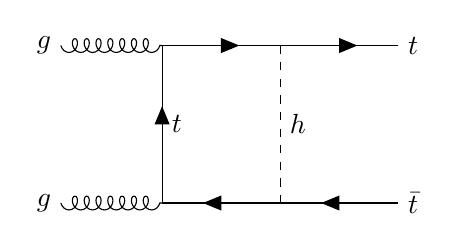
\begin{tikzpicture}
      \begin{feynman}
        \vertex (i1) {\(g\)};
        \vertex [below=2.0 cm of i1] (i2) {\(g\)};
        \vertex [right=1.5 cm of i1] (a);
        \vertex [right=1.5 cm of i2] (b);
        \vertex [right=1.5 cm of a] (c);
        \vertex [right=1.5 cm of b] (d);
        \vertex [right=1.5 cm of c] (f1) {\(t\)};
        \vertex [right=1.5 cm of d] (f2) {\(\bar{t}\)};
        \diagram* {
          (i1) -- [gluon] (a),
          (i2) -- [gluon] (b),
          (c) -- [scalar, edge label=\(h\)] (d),
          (f1) -- [anti fermion] (c) -- [anti fermion] (a) -- [anti fermion, edge label=\(t\)] (b) -- [anti fermion] (d) -- [anti fermion] (f2)
        };
      \end{feynman}
    \end{tikzpicture}
    \caption{\textbf{EW correction involving a SM Higgs boson.} An example Feynman diagram for NLO EW corrections to \ttbar production involving the exchange of a virtual SM Higgs boson $h$.}
    \label{fig:ah:ewcorr_feynman}
\end{figure}

The NLO corrections in the electroweak coupling \alphaew are computed with the HATHOR code~\cite{Aliev:2010zk, Kuhn:2005it, Kuhn:2006vh, Kuhn:2013zoa} using the same nominal scale choices. Of particular interest here is a class of diagrams which contain an exchange of a virtual SM Higgs boson, an example of which is seen in \cref{fig:ah:ewcorr_feynman}. The matrix element for this diagram is proportional to the square of the SM Higgs-top Yukawa coupling \yt, giving a $\yt^2$-dependent correction to \ttbar distributions from the interference with LO diagrams. This correction is sizeable mostly for low \mtt values, and is important for this analysis because the SM Higgs exchange might change the \ttbar spin state and thus \chel and \chan. To accurately account for this, the correction is derived separately for the different initial states ($gg$, $q\bar{q}$ and $gq$) of \ttbar production.

The results obtained with HATHOR are accurate only to LO in \alphas, i.e. \order{\alphas^2}, and as of the time of writing no full calculation including both NLO QCD and EW effects exists. Thus, there is an ambiguity on how the NLO-accurate (in QCD) MC simulation and the NNLO-accurate corrections presented in the previous section should be combined with the EW corrections.

Formally, the differential cross section as predicted by Powheg can be decomposed as

\begin{equation}
    d \sigma_{\powheg} = \alphas^2 d \sigma_{\mathrm{LO}} + \alphas^3 d \sigma_{\mathrm{NLO}}
\end{equation}

\noindent where additional terms beyond $\order{\alphas^3}$ due to additional radiation in Powheg and Pythia are not written for simplicity. On the other hand, HATHOR predicts

\begin{equation}
    d \sigma_{\mathrm{HATHOR}} = \alphas^2 d \sigma_{\mathrm{LO}} + \alphas^2 \alphaew d \sigma_{\mathrm{EW}}.
\end{equation}

One possible way to combine the calculations is the additive scheme, given by


\begin{equation}
\begin{split}
\label{eq:ah:ewadd}
    d \sigma_{\mathrm{add.}} &= d \sigma_{\powheg} + d \sigma_{\mathrm{HATHOR}} - \alphas^2 d \sigma_{\mathrm{LO}} \\
    &= \alphas^2 d \sigma_{\mathrm{LO}} + \alphas^3 d \sigma_{\mathrm{NLO}} + \alphas^2 \alphaew d \sigma_{\mathrm{EW}}
\end{split}
\end{equation}

\noindent which is formally accurate to $\order{\alphas^3}$ and $\order{\alphas^2 \alphaew}$. This approach does not include any cross terms of order $\order{\alphas^3 \alphaew}$, which are not fully calculated by either Powheg or HATHOR. However, it is reasonable to assume that these cross terms factorize approximately, leading to the alternative multiplicative scheme~\cite{Kuhn:2013zoa}

\begin{equation}
\begin{split}
\label{eq:ah:ewmult}
    d \sigma_{\mathrm{mult.}} &= d \sigma_{\powheg} \times \frac{d \sigma_{\mathrm{HATHOR}}} {\alphas^2 d \sigma_{\mathrm{LO}}} \\
    &= \alphas^2 d \sigma_{\mathrm{LO}} + \alphas^3 d \sigma_{\mathrm{NLO}} + \alphas^2 \alphaew d \sigma_{\mathrm{EW}} + \alphas^3 \alphaew \frac {d \sigma_{\mathrm{NLO}} \, d \sigma_{\mathrm{EW}}}{d \sigma_{\mathrm{LO}}}
\end{split}
\end{equation}

The difference between the two schemes is in the last term of order $\order{\alphas^3\alphaew}$, which is an approximation to the QCD-EW cross terms. In this work, the multiplicative approach is used for all nominal results, while the difference to the additive approach is included as a systematic uncertainty. In both cases, the needed term $d \sigma_{\mathrm{LO}}$ is computed with MadGraph 5.

The effect of both approaches on the 3D \mttchelchan distribution at the detector level after parton showering can be seen in \cref{fig:ah:ewqcdcorrs} for different values of \yt. The multiplicative scheme leads to a larger correction of roughly $2-4\%$, while the additive scheme only gives $1-2\%$. Notably, the effect of varying \yt modifies not only the \mtt distribution close to the \ttbar threshold, but also the distribution of \chel. As a result, such a variation in data could potentially be confused for a pseudoscalar signal. It is thus important to include it as a systematic uncertainty, as described in \cref{sec:ah:systs}.


\section{Matrix element reweighting for \AH signals}
\label{sec:ah:mereweighting}

In order to probe the full phase space of the generic \AH model as described in \cref{sec:ah:intro}, predictions at different \AH masses and widths with a sufficiently small spacing are required so that interpolation between the points is possible. However, generating a separate MC sample for each mass and width point is computationally very expensive.

\subsection{Principle of the method}

As an alternative, it is possible to re-use existing samples for different mass and width points via matrix-element reweighting. This method works by noting that a given MC sample can be seen as a random sample, drawn from a PDF of the form

\begin{equation}
\label{eq:ah:merewprob}
    \mathcal{P}(x_i^{\mathrm{ME}}, x_j^{\mathrm{reco}}) = \mathcal{P}^{\mathrm{ME}} (x_i^{\mathrm{ME}}) \cdot \mathcal{P}^{\mathrm{rem}} (x_j^{\mathrm{reco}} | x_i^{\mathrm{ME}})
\end{equation}

Here, $x_i^{\mathrm{ME}}$ are all variables defining the event at the matrix element (ME) level, i.e. at the level of the hard interaction, and $x_j^{\mathrm{reco}}$ are all variables after detector simulation and object reconstruction. For the case of the \AH signals, which are generated at LO in QCD, $x_i^{\mathrm{ME}}$ is given fully by the four-momenta and helicities of the final-state particles (leptons, neutrinos and b quarks) in the hard process. The $x_j^{\mathrm{reco}}$ consist of all possible reconstruction-level variables that are relevant to the analysis, such as e.g. jet and lepton four-momenta, lepton identification criteria or \ptmissvec. 

$\mathcal{P}^{\mathrm{ME}} (x_i^{\mathrm{ME}})$ refers to the probability density of the ME-level variables as predicted by the ME generator, which will be proportional to the absolute square of the matrix element. This function will depend on the chosen scenario of the \AH model, i.e. $m_{\AH}$ and $\Gamma_{\AH}$. Meanwhile, the conditional probability density $\mathcal{P}^{\mathrm{rem}} (x_j^{\mathrm{reco}} | x_i^{\mathrm{ME}})$ encodes the effects of all other components of the simulation chain, such as the parton shower, hadronization, detector simulation and reconstruction. It gives the probability to observe reconstruction-level variables $x_j^{\mathrm{reco}}$ for an event with ME-level variables $x_i^{\mathrm{ME}}$.

The principal assumption of the method is now that $\mathcal{P}^{\mathrm{rem}}$, and thus the whole simulation chain except for the matrix element, is independent of the underlying \AH signal scenario ($m_{\AH}$ and $\Gamma_{\AH}$). This assumption is certainly true for the detector simulation and reconstruction, while care must be taken for the parton shower, which in general needs to be matched to the matrix element and can this way have a residual dependence. The validity of the assumption will be discussed in more detail below.

If the assumption is fulfilled, a given \AH MC sample generated with parameters $m_{\AH}^0$ and $\Gamma_{\AH}^0$ can now be reweighted to a different \AH scenario with parameters $\hat{m}_{\AH}$ and $\hat{\Gamma}_{\AH}$ by applying to each event $i$ a weight 

\begin{equation}
\label{eq:ah:merewweight}
    w_i = \frac{ \mathcal{P}^{\mathrm{ME}} (x_i^{\mathrm{ME}} | \hat{m}_{\AH} , \hat{\Gamma}_{\AH} ) } { \mathcal{P}^{\mathrm{ME}} (x_i^{\mathrm{ME}} | m_{\AH}^0 , \Gamma_{\AH}^0 ) }
\end{equation}

The quantities in the denominator and nominator are the ME-level probability densities for each event, evaluated at the original and target \AH parameters, respectively. When this weight is inserted into \cref{eq:ah:merewprob}, the original probability cancels, giving the correct probability density for the target scenario $\hat{m}_{\AH}$ and $\hat{\Gamma}_{\AH}$.

In practice, this method will only work if the MC sample used for the reweighting has sufficient phase space overlap with the target \AH scenario, i.e. if the two probabilities in \cref{eq:ah:merewweight} are not too different from each other for the majority of the events. Otherwise, the weights will become very small in some regions of the phase space and very large in others, resulting in poor statistics for the reweighted sample.

The method was implemented by directly evaluating the squared matrix elements for the different \AH hypotheses, using the standalone reweighting interface provided by MadGraph 5 and the same UFO model as for the signal generation. 

\subsection{Combination of multiple origin samples}

For the purpose of this analysis, a set of signal samples for different \AH scenarios (as given in \cref{sec:ah:datasets}) was already available at the time of starting these studies. These samples were used as origin samples for the reweighting. In order to maximize the statistics achieved after reweighting for each target \AH scenario, and mitigate problems from poor phase space overlap, a subset of the available samples were combined after reweighting for each target scenario.

This procedure works as follows: First, a set of several origin samples $j$ with different parameters $m_{\AH}$ and $\Gamma_{\AH}$ are all reweighted separately to the same target parameters $\hat{m}_{\AH}$ and $\hat{\Gamma}_{\AH}$ with per-event weights $w_{i,j}$ as given in \cref{eq:ah:merewweight}. Then, the different samples are again weighted with a per-sample weight $v_j$ proportional to

\begin{equation}
    v_j \propto {\langle w_{i,j} \rangle}^{-1} =  \frac{ \sum_i w_{i,j} }{ \sum_i w_{i,j}^2 }
\end{equation}

\noindent where the sums run over all events $i$ in the considered sample $j$. This expression is the inverse of the average ME weight for sample $j$. It is chosen such that samples with large phase space overlap with the target \AH scenario - and thus small ME weights $w_{i,j}$ - are assigned a large weight $v_j$ in the combination of samples. Similarly, samples with poor phase space overlap, and thus large average ME weights, get assigned small weights and contribute less strongly to the combined sample. Finally, the total combined sample is normalized to the expected cross section for the target scenario, which is calculated independently. It can be shown that this procedure minimizes the total statistical error of the combined sample.

In practice, all available masses and parities (A and H) are combined for each target \AH mass. Resonance and interference contributions are treated separately from each other. Furthermore, it was found that, for the resonance contribution only, it is necessary to split the combination of different \AH widths into two halves: those with $\wAH/\mAH$ less or greater than 10\%. This is due to an interplay of \madgraph and the \pythia shower leading to a dependency on the \AH width in the matrix element, which is not taken into account in the reweighting. For $\wAH/\mAH < 10\%$ (narrow resonance), \madgraph includes the the intermediate \AH particle in the event record, which is then treated by \pythia as a unstable resonance and its virtuality as predicted by the matrix element is preserved. For $\wAH/\mAH \geq 10\%$ (broad resonance), the \AH particle is not included in the event record, and its virtuality is thus not preserved. This leads to slight differences in distributions affected by the parton showering. The choice of 10\% for the transition between the two modes is an arbitrary parameter, and thus not necessarily physical. Nonetheless, it was decided in this analysis to not mix the two width ranges in the reweighting in order to obtain full closure with a stand-alone generation.

\subsection{Validation}

The combined reweighting is validated for three masses of $\mAH = 400$, 600 and 800 GeV as well as widths of 2.5 and 10\%. For each of these points, the reweighting is performed as stated above, but leaving out \AH scenarios with the same mass from the combination of origin samples since otherwise the weights would be trivially one. The reweighted \mtt distributions at generator level are then compared to the stand-alone samples at the same \mAH and \wAH.

The resulting comparisons and residuals can be seen in \cref{fig:ah:merew_validation_A,fig:ah:merew_validation_H} for A and H, respectively, separated into the resonance and interference contributions. It can be seen that the closure between reweighting and standalone generation is excellent within the statistical uncertainties.

\begin{figure}[!p]
    \centering
    \begin{subfigure}[b]{0.49\textwidth}
        \centering
        \includegraphics[width=\textwidth]{figures/ah/me_reweighting/A_res_2p5_mtt_log_pos.pdf}
        \caption{A, $\wA/\mA = 2.5\%$, resonance}
    \end{subfigure}
    \hfill
    \begin{subfigure}[b]{0.49\textwidth}
        \centering
        \includegraphics[width=\textwidth]{figures/ah/me_reweighting/A_res_10p0_mtt_log_pos.pdf}
        \caption{A, $\wA/\mA = 10\%$, resonance}
    \end{subfigure}
    \begin{subfigure}[b]{0.49\textwidth}
        \centering
        \includegraphics[width=\textwidth]{figures/ah/me_reweighting/A_int_2p5_mtt_diff.pdf}
        \caption{A, $\wA/\mA = 2.5\%$, interference}
    \end{subfigure}
    \hfill
    \begin{subfigure}[b]{0.49\textwidth}
        \centering
        \includegraphics[width=\textwidth]{figures/ah/me_reweighting/A_int_10p0_mtt_diff.pdf}
        \caption{A, $\wA/\mA = 10\%$, interference}
    \end{subfigure}
    \caption{\textbf{Validation of the ME reweighting for A.} Comparison of standalone generated (solid) and reweighted (dashed) \mtt distributions for different values of \mA. The lower panel shows the ratio of reweighted and standalone distributions. The error bars and colored areads give the statistical uncertainty of the reweighted and standalone sample, respectively.}
    \label{fig:ah:merew_validation_A}
\end{figure}

\begin{figure}[!p]
    \centering
    \begin{subfigure}[b]{0.49\textwidth}
        \centering
        \includegraphics[width=\textwidth]{figures/ah/me_reweighting/H_res_2p5_mtt_log_pos.pdf}
        \caption{H, $\wH/\mH = 2.5\%$, resonance}
    \end{subfigure}
    \hfill
    \begin{subfigure}[b]{0.49\textwidth}
        \centering
        \includegraphics[width=\textwidth]{figures/ah/me_reweighting/H_res_10p0_mtt_log_pos.pdf}
        \caption{H, $\wH/\mH = 10\%$, resonance}
    \end{subfigure}
    \begin{subfigure}[b]{0.49\textwidth}
        \centering
        \includegraphics[width=\textwidth]{figures/ah/me_reweighting/H_int_2p5_mtt_diff.pdf}
        \caption{H, $\wH/\mH = 2.5\%$, interference}
    \end{subfigure}
    \hfill
    \begin{subfigure}[b]{0.49\textwidth}
        \centering
        \includegraphics[width=\textwidth]{figures/ah/me_reweighting/H_int_10p0_mtt_diff.pdf}
        \caption{H, $\wH/\mH = 10\%$, interference}
    \end{subfigure}
    \caption{\textbf{Validation of the ME reweighting for H.} Comparison of standalone generated and reweighted \mtt distributions for different values of \mH, similar to \cref{fig:ah:merew_validation_A}.}
    \label{fig:ah:merew_validation_H}
\end{figure}

\section{Systematic uncertainties}
\label{sec:ah:systs}

Similar to \cref{sec:ttxs:systematics}, systematic uncertainties affect the distributions of both SM background and signal processes. They are listed in this section, split into theory (\cref{sec:ah:theorysysts}) and experimental uncertainties (\cref{sec:ah:expsysts}).

\subsection{Theory uncertainties}
\label{sec:ah:theorysysts}

\paragraph{Scale uncertainties.}
Uncertainties due to missing higher orders in the matrix element as well as the parton shower are included separately for the SM \ttbar, tW, \Zgamma+jets backgrounds as well as all considered signals by varying the associated scales by a factor 2 up and down independently, same as in \cref{sec:ttxs:systematics}. For A and H, the uncertainties are considered uncorrelated between the resonance and interference components, which is found to be conservative. For \etat, the renormalization scale uncertainty is not included since the considered model does not encode any dependence on either $\mu_R$ or \alphas.

\paragraph{PDF uncertainties.}
For the SM \ttbar background, the uncertainty due to the PDF is again included based on the 100 provided eigenvalues of the used NNPDF 3.1 PDF set. However, it is not considered sufficient to simply take the envelope of these variations since this would distort possible shape variations. Instead, a principal component analysis (PCA) is performed on the final 3D templates obtained from the different eigenvalues, thus finding those linear combinations that have a noticable shape effect. It is found that only the first eigenvector (corresponding to the largest eigenvalue) is non-negligible, and variation is considered as the PDF uncertainty. Independently of this, another uncertainty based on the value of \alphas in the PDF is considered similarly to \cref{sec:ttxs:systematics}.

\paragraph{EW correction uncertainties.}
As described in \cref{sec:ah:ewcorr}, two independent uncertainties are attached to the NLO electroweak correction of SM {\ttbar}: First, the value of the SM top-Higgs Yukawa coupling is allowed to vary in the range $\yt = {1.00}^{+0.11}_{-0.11}$, with the range given by the uncertainty of the experimental measurement in \citere{CMS:HIG-17-031}. Second, the difference between the additive and multiplicative application scheme (\cref{eq:ah:ewadd,eq:ah:ewmult}) is considered as a seperate uncertainty, as recommended in \citere{Kuhn:2013zoa}, and symmetrized around the nominal.

\paragraph{Top quark mass uncertainty.}
The top quark mass uncertainty in SM \ttbar is estimated by varying it from its nominal value of $\mt = \SI{172.5}{\GeV}$ by $\pm \SI{3}{\GeV}$ in the \powheg simulation, and then scaling down the resulting relative deviation by a factor $1/3$, leading to a $\pm \SI{1}{\GeV}$ uncertainty. This is done since the variation, obtained from an independent MC sample, is otherwise plagued by large statistical uncertainties. Furthermore, the top mass is also varied in all considered signal samples directly by $\pm \SI{1}{\GeV}$ through an ME reweighting method similar to \cref{sec:ah:mereweighting}. The top mass uncertainties between background and signals are considered as fully correlated.

\paragraph{Further uncertainties in SM \ttbar.}
Additionally, separate SM \ttbar samples are used to evaluate uncertainties due to ME/PS matching (same as in \cref{sec:ttxs:systematics}), the underlying event tune~\cite{CMS:GEN-17-001}, and the color reconnection model in \pythia~\cite{CMS:GEN-17-002,Christiansen:2015yqa}. All of these effects are found to be small in the channels considered here.

\paragraph{Background cross section uncertainties.}
For the SM \ttbar background, instead of including an explicit cross section uncertainty, the shift in the predicted NNLO+NNLL \ttbar cross section due to the ME scales and the top quark mass is correlated with the respective uncertainties. For minor backgrounds, explicit uncertainties of 15\% for tW and t-channel single top, 30\% for diboson and \ttbar+X, and 5\% for the data-driven \Zgamma+jets normalization are considered.

\paragraph{Background statistical uncertainties.}
Again similar to \cref{sec:ttxs:systematics}, per-bin background statistical uncertainties for all simulated processes are included following \citere{Barlow:1993dm}.

\subsection{Experimental uncertainties}
\label{sec:ah:expsysts}

\paragraph{Jet and \ptmiss uncertainties.}
The uncertainty on the calibration of the jet \pt detector response is split into five subsources, of which three are considered uncorrelated between years and two (related to the response to jets of different flavor) are correlated. Further subsources as provided by CMS are found to be negligible for this analysis. Furthermore, the uncertainty in the jet \pt resolution is considered separately, again uncorrelated between years. All jet uncertainties are fully propagated to the calculation of \ptmiss, and an additional \ptmiss uncertainty based on soft, unclustered hadronic activity is also considered.

\paragraph{b tagging uncertainties.}
Similarly, the uncertainty on the b tagging efficiency is split into 17 subsources, corresponding e.g. to different parton shower modeling, the treatment of leptons in the jet, or the propagation of the jet \pt scale uncertainties. One component represents the statistical uncertainty and is thus considered uncorrelated, while all others are correlated among years. Moreover, the uncertainty on mistagging of light-flavor jets is included, also split into a statistical and a systematic component.

\paragraph{Lepton and trigger uncertainties.}
Uncertainties on the lepton reconstruction, identification and isolation efficiencies, as measured centrally in CMS using the tag-and-probe method, are considered seperately for muons and electrons~\cite{CMS:EGM-17-001,CMS:MUO-16-001}. For the muons, the uncertainty is split into a statistical component (uncorrelated between the analysis years) and a systematic component (correlated). Similarly, the dilepton trigger efficiency uncertainties are considered uncorrelated between years and lepton flavor channels. Finally, in data taken in 2016 or 2017, an additional uncertainty is assigned due to an inefficiency in the ECAL L1 trigger~\cite{CMS:TRG-17-001}, as described in \cref{sec:ah:expcorrs}.

\paragraph{Luminosity uncertainty.}
The uncertainty on the total integrated luminosity is included following \citeres{CMS:LUM-17-003,CMS:LUM-17-004,CMS:LUM-18-002}, leading to a total luminosity uncertainty of $1.6\%$, split into a total of seven components with different correlations between the years.

\paragraph{Pileup uncertainty.}
To estimate the uncertainty on the amount of pileup per pp bunch crossing, the effective inelastic proton-proton cross section used for pileup reweighting in the simulation is varied by 4.6\% from its nominal value.

\subsection{Differences between MC generators}
\label{sec:ah:gennps}

It has been observed in previous analyses that the theoretical uncertainties collected in \cref{sec:ah:theorysysts} do not necessarily cover the differences in the predictions of different MC generators for \ttbar~\cite{ATLAS:2018ivx,CMS:TOP-17-002,CMS:TOP-23-001,ATLAS:2023fsd}. To assess the size of these effects, the standard \ttbar prediction as computed using \powheg \hvq matched to \pythia is compared to alternate generator setups.%, namely:

%\begin{itemize}
%    \item \powheg \hvq matched to \herwig;
%    \item \amcatnlo matched to \pythia;
%    \item \powheg \bbfourl matched to \pythia.
%\end{itemize}

The first of these is the same \powheg \hvq matrix element matched to the multi-purpose envent generator \herwig instead of \pythia. The angular-ordered parton shower in \herwig is used (as opposed to the \pt-ordered dipole shower in \pythia) together with the CMS CH3 tune~\cite{CMS:GEN-19-001}. Furthermore, \herwig uses a cluster hadronization model~\cite{Webber:1983if} instead of the string hadronization model of \pythia as described in \cref{sec:mc:hadronization}.

\begin{figure}[!t]
    \centering
    \includegraphics[width=0.49\textwidth]{figures/ah/altbgs/pyvshw_mtt.pdf}
    \hfill
    \includegraphics[width=0.49\textwidth]{figures/ah/altbgs/pyvshw_chel_lowmtt.pdf}
    \caption{
        \textbf{Comparison of \herwig and \pythia.} The ratio of the predictions of \powheg \hvq \ttbar matched to \herwig and to \pythia for the inclusive reconstructed \mtt distribution (left) and the reconstructed \chel distribution, restricted to $\mtt < \SI{360}{\GeV}$ (right). The effect of the \etat signal is also shown for comparison.
    }
    \label{fig:ah:herwig}
\end{figure}

\Cref{fig:ah:herwig} shows the ratios of the predictions from \herwig and \pythia for the reconstructed \mtt distribution, as well as for the \chel distribution close to the \ttbar threshold (i.e. where the \etat signal is located). Besides a significantly lower \ttbar acceptance, \herwig predicts an increase of events at the \ttbar threshold similar to \etat.
This appears concerning at first glance since, should the data follow the prediction from \herwig instead of \pythia, this enhancement could be confused with an \etat signal if \pythia is used as the baseline prediction.
However, as seen in \cref{fig:ah:herwig} on the right, \herwig at the same predicts a flatter slope in \chel than \pythia, equivalent to less \ttbar spin correlation\footnote{This effect was also seen in the context of \citere{ATLAS:2023fsd}.}. This is in contrast to the \etat signal, in which the \ttbar spins are maximally anticorrelated. The inclusion of the spin correlation variable \chel in the analysis thus makes it possible to separate the differences between \powheg and \herwig with respect to \etat.

The second alternative generator is \bbfourl matched to \pythia, as studied extensively in \cref{ch:bb4l}. Here, particularly the off-shell effects included in \bbfourl might be of interest for the extraction of \etat since the latter is located below the \ttbar threshold. The setup denoted as ``\bbfourl v2'' in \cref{sec:bb4l:bb4l}, corresponding to \citere{Jezo:2023rht}, is used, and compared to the sum of the \powheg \hvq \ttbar and tW predictions for consistency.

A caveat here is presented by the corrections to NNLO QCD and NLO EW as described in \cref{sec:ah:ttbarweights}. These are derived from fixed-order corrections assuming stable top quarks, and are not available for the full \bbllnunu final state. To still be able to apply them to \bbfourl predictions, the \bbfourl sample is split into a \ttbar and a tW part in an ad-hoc way by using the matrix element history projectors implemented in \bbfourl~v2~\cite{Jezo:2023rht}. The corrections are then applied to the \ttbar part only in the same manner as to \powheg \hvq.

\begin{figure}[!t]
    \centering
    \includegraphics[width=0.49\textwidth]{figures/ah/altbgs/hvqvsbb4l_mtt.pdf}
    \hfill
    \includegraphics[width=0.49\textwidth]{figures/ah/altbgs/hvqvsbb4l_chel_lowmtt.pdf}
    \caption{
        \textbf{Comparison of \powheg \tttWsum and \bbfourl.} The ratio of the predictions of the sum of \powheg \hvq \ttbar and tW to \bbfourl (all matched to \pythia) for the inclusive reconstructed \mtt distribution (left) and the reconstructed \chel distribution, restricted to $\mtt < \SI{360}{\GeV}$ (right). The effect of the \etat signal is also shown for comparison.
    }
    \label{fig:ah:bb4l}
\end{figure}

The ratios of the predictions are shown in \cref{fig:ah:bb4l} in the same manner as before. It can be seen that \bbfourl does not predict major differences in the reconstructed \mtt spectrum even at its lower edge. However, it results in a significantly steeper slope in reconstructed \chel close to the threshold. This increase in slope is of similar magnitude as the effect expected due to \etat. 

The source of this difference is not yet fully understood. \bbfourl contains NLO QCD corrections to the top decay which are not present in \hvq (though they are approximated through the matrix element corrections in \pythia). However, NLO corrections to spin correlations are expected to not only be small, but reduce the spin correlation instead of enhancing it~\cite{Bernreuther:2004jv}. It is possible that the effect instead originates in the \tttW interference: The tW contribution on its own is expected to have approximately flat \chel since one of the leptons is not actually the decay product of a top quark, and the interference between \ttbar and tW is destructive in large parts of the phase space. If the interference in \bbfourl is now larger than in \tttWsum, it could thus reduce the contribution from tW, effectively enhancing the \chel slope. Since \ttbar and tW are not cleanly separable in \bbfourl, however, this hypothesis is difficult to confirm, and such studies are beyond the scope of this analysis.

%For the purpose of the \etat extraction, the differences to these alternative generator setups are included in the fit as two additional shape-based nuisance parameters (one for \pythia compared to \herwig, and one for \tttWsum compared to \bbfourl). In both cases, the \powheg \hvq + \pythia prediction is considered the nominal, and the alternate prediction is considered the $+1\sigma$ template. The $-1\sigma$ template is constructed by symmetrizing the relative difference around the nominal, and intermediate values are obtained by interpolation as usual. \todo{where are the NPs used and where not}

A third alternative prediction is provided by \ttbar+jets production simulated with \amcatnlo, matched to \pythia with the FxFx scheme~\cite{Frederix:2012ps}. While this prediction is formally also NLO-accurate in QCD in the NWA, and thus comparable to \powheg \hvq, it has been observed in past measurements that \amcatnlo does not agree as well with data as \powheg for \ttbar production. As a result, \amcatnlo is given less focus compared to the other two predictions in this work.

In this work, \powheg \hvq + \pythia is considered for the nominal background prediction in all cases. A comparison to \powheg \hvq + \herwig, \amcatnlo + \pythia, and \bbfourl + \pythia is shown in \cref{sec:ah:checks} in the context of measuring the \etat cross section. Furthermore, the effect of including the differences to \powheg \hvq + \herwig and \bbfourl + \pythia as two additional shape-based nuisance parameters in the fit is similarly given in \cref{sec:ah:checks}. Note that in \citere{CMS:TOP-24-007}, these nuisance parameters were considered as part of the main result in order to be conservative with respect to the total uncertainty.

\subsection{Uncertainty smoothing}
Several of the considered uncertainty sources, e.g. the top quark mass in SM \ttbar, are estimated by either comparing to separate MC samples, which causes the relative deviation due to the source to be affected by large statistical noise. A similar problem appears for uncertainties which effectively vary the cuts applied on MC events, such as e.g. the jet \pt scale uncertainties by way of jet acceptances. If left untreated, fitting these noisy shape templates to the data could lead to erroneous constraints in the likelihood fit. To prevent this, the smoothing algorithm LOWESS~\cite{Cleveland:1979,Cleveland:1988} is applied to the relative deviations for these sources, with the bandwidth used for the smoothing determined separately through cross-validation for each source. For more details on the procedure, see \citere{Anuar:PhD}.

\section{Pre-fit distributions}
\label{sec:ah:prefit}

\begin{figure}[!hp]
    \centering
    \includegraphics[width=0.49\textwidth]{figures/ah/controlplots/Req MET/sf/Leptonpt_Req MET_sf.pdf}
    \hfill
    \includegraphics[width=0.49\textwidth]{figures/ah/controlplots/Req MET/em/Leptonpt_Req MET_em.pdf}
    \includegraphics[width=0.49\textwidth]{figures/ah/controlplots/Req MET/sf/Leptoneta_Req MET_sf.pdf}
    \hfill
    \includegraphics[width=0.49\textwidth]{figures/ah/controlplots/Req MET/em/Leptoneta_Req MET_em.pdf}
    \includegraphics[width=0.49\textwidth]{figures/ah/controlplots/Req MET/sf/deltaphi_Req MET_sf.pdf}
    \hfill
    \includegraphics[width=0.49\textwidth]{figures/ah/controlplots/Req MET/em/deltaphi_Req MET_em.pdf}
    \caption{
        \textbf{Control distributions.} Shown are the distributions of \pt of both leptons (top), $\eta$ of both leptons (center), and the azimuthal angle \dphill between the leptons (bottom) in the \ee/\mumu (left) and \emu channels (right). All figures show both data (black dots) and different simulated background processes (colored bars), as well as the statistical uncertainty only. 
    }
    \label{fig:ah:control1}
\end{figure}

\begin{figure}[!hp]
    \centering
    \includegraphics[width=0.49\textwidth]{figures/ah/controlplots/Req MET/sf/Jetpt_Req MET_sf.pdf}
    \hfill
    \includegraphics[width=0.49\textwidth]{figures/ah/controlplots/Req MET/em/Jetpt_Req MET_em.pdf}
    \includegraphics[width=0.49\textwidth]{figures/ah/controlplots/Req MET/sf/Jeteta_Req MET_sf.pdf}
    \hfill
    \includegraphics[width=0.49\textwidth]{figures/ah/controlplots/Req MET/em/Jeteta_Req MET_em.pdf}
    \includegraphics[width=0.49\textwidth]{figures/ah/controlplots/Req MET/sf/njet_Req MET_sf.pdf}
    \hfill
    \includegraphics[width=0.49\textwidth]{figures/ah/controlplots/Req MET/em/njet_Req MET_em.pdf}
    \caption{
        \textbf{Control distributions.} Shown are the distributions of \pt of all jets (top), $\eta$ of all jets (center), and the number of jets (bottom) in the \ee/\mumu (left) and \emu channels (right). All figures show both data (black dots) and different simulated background processes (colored bars), as well as the statistical uncertainty only. 
    }
    \label{fig:ah:control2}
\end{figure}

\begin{figure}[!hp]
    \centering
    \includegraphics[width=0.49\textwidth]{figures/ah/controlplots/Req MET/sf/METpt_Req MET_sf.pdf}
    \hfill
    \includegraphics[width=0.49\textwidth]{figures/ah/controlplots/Req MET/em/METpt_Req MET_em.pdf}
    \includegraphics[width=0.49\textwidth]{figures/ah/controlplots/Req MET/sf/mll_Req MET_sf.pdf}
    \hfill
    \includegraphics[width=0.49\textwidth]{figures/ah/controlplots/Req MET/em/mll_Req MET_em.pdf}
    \includegraphics[width=0.49\textwidth]{figures/ah/controlplots/Reco/sf/mbbll__sf.pdf}
    \hfill
    \includegraphics[width=0.49\textwidth]{figures/ah/controlplots/Reco/em/mbbll__em.pdf}
    \caption{
        \textbf{Control distributions.} Shown are the distributions of \ptmiss (top), \mll (center), and the invariant mass \mbbll of both b candidates and both leptons  (bottom) in the \ee/\mumu (left) and \emu channels (right). All figures show both data (black dots) and different simulated background processes (colored bars), as well as the statistical uncertainty only. 
    }
    \label{fig:ah:control3}
\end{figure}

\begin{figure}[!hp]
    \centering
    \includegraphics[width=0.49\textwidth]{figures/ah/controlplots/Reco/ll/toppt_Reco_ll.pdf}
    \hfill
    \includegraphics[width=0.49\textwidth]{figures/ah/controlplots/Reco/ll/topeta_Reco_ll.pdf}
    \includegraphics[width=0.49\textwidth]{figures/ah/controlplots/Reco/ll/costhetastar__ll.pdf}
    \hfill
    \includegraphics[width=0.49\textwidth]{figures/ah/controlplots/Reco/ll/mtt_Reco_ll.pdf}
    \includegraphics[width=0.49\textwidth]{figures/ah/controlplots/Reco/ll/chel__ll.pdf}
    \hfill
    \includegraphics[width=0.49\textwidth]{figures/ah/controlplots/Reco/ll/chan__ll.pdf}
    \caption{
        \textbf{Control distributions after \ttbar reconstruction.} Shown are (from top left to bottom right) the distributions of the top quark \pt, top quark $\eta$, \mtt, \cost, \chel and \chan for the sum of all dilepton channels. All figures show both data (black dots) and different simulated background processes (colored bars), as well as the statistical uncertainty only. 
    }
    \label{fig:ah:controlttbar}
\end{figure}

The agreement between the total MC prediction, including all corrections described in \cref{sec:ah:expcorrs,sec:ah:ttbarweights}, and the observed data are presented in this section. Shown observables are lepton \pt, $\eta$ and \dphill (\cref{fig:ah:control1}), jet \pt, $\eta$ and count (\cref{fig:ah:control2}), \ptmiss, and the invariant masses of the two leptons \mll and of the two leptons and two b-tagged jets \mbbll (\cref{fig:ah:control3}). All of them are shown after all lepton, jet, b tag and \ptmiss requirements, but before the \ttbar reconstruction, summed over all analysis years, and separately for the same-flavor (\ee and \mumu) and opposite-flavor (\emu) channels, since the latter have different backgrounds and cuts.

It can be seen that there is a slight but consistent overprediction of the background normalization compared to the data in almost all distributions. Furthermore, there is a slight slope in the ratio of data and simulation yields in some energy-related observables like lepton or jet \pt. Both of these discrepencies are well covered by systematic uncertainties \todo{make sure this is the case}.

Furthermore, different distributions resulting from the \ttbar reconstruction (see \cref{sec:ah:kinreco}) are shown in \cref{fig:ah:controlttbar}, this time summed also over lepton flavor. They consist of top quark \pt, $\eta$ and scattering angle \cost as well as the three observables used for the fit, \mtt, \chel and \chan.



Finally, the three-dimensional \mttchelchan distribution used for the statistical analysis is shown before the fit, including all systematic uncertainties, in \cref{fig:ah:prefit_ll}. A notable excess of the data compared to the prediction is observed for low values of \mtt, consistent with the excess seen in the one-dimensional \mtt distribution (\cref{fig:ah:controlttbar}) and in the related observables \mll and \mbbll (\cref{fig:ah:control3}). The excess is stronger for large values of \chel as seen from the multi-dimensional binning, while no trend can be seen by eye regarding \chan.

\begin{figure}[t]
    \centering
    \includegraphics[width=0.99\textwidth]{figures/ah/prepost/A_m365_w2p0__H_m365_w2p0_fit_p_ll_run2_both.pdf}
    \caption{
        \textbf{Prefit distributions of \mttchelchan.} The unrolled three-dimensional distribution in \mtt, \chel and \chan as used for statistical analysis before the fit to the data, summed over all years and lepton flavors. The upper panel shows the sum of the background simulation (colored bars) and the observed data (black dots), while the lower panel shows the ratio of the data to the prediction, with different signals overlaid: A (red) and H (blue), both for $\mAH = \SI{365}{\GeV}$ and $\wAH/\mAH = 2\%$, and \etat (green).
    }
    \label{fig:ah:prefit_ll}
\end{figure}

%\section{Extraction of non-perturbative effects in \ttbartitle}
%\label{sec:ah:etat}

\section{Interpretation of the excess}
\label{sec:ah:excess}

\subsection{Extraction of \ttbartitle bound state effects}
\label{sec:ah:etat}

The prefit excess visible in \cref{fig:ah:prefit_ll} is interpreted in terms of a pseudoscalar \ttbar bound state by performing a signal+background fit with \etat as the signal, as defined in \cref{sec:theory:etat}. The POI in the fit is \sigetat, the cross section of the \etat model, which can be understood as the difference between the data and the FO pQCD background prediction. It is measured to be

\begin{equation}
    %\sigetat = 8.8^{+1.2}_{-1.4} \, \si{\pb}.
    \sigetat = 8.7 \pm 0.5 (\text{stat}) \pm 1.0 (\text{syst}) \, \si{\pb} = 8.7 \pm 1.1  \, \si{\pb}.
\end{equation}

Here, the statistical component of the uncertainty is estimated by fixing all nuisance parameters to their postfit values, while the systematic component is obtained as the quadratic difference between the total and the statistical uncertainty. The significance of the result compared to a background-only hypothesis, i.e. without a bound state, is more than five standard deviations.

The result is of a similar order of magnitude as the prediction of \SI{6.43}{\pb} given in \citere{Fuks:2021xje}, obtained by fitting the results of an NRQCD calculation from \citere{Sumino:2010bv}, though this result is not one-to-one comparable since it considers only the range of $\mtt \in [338, 350] \, \si{\GeV}$. 

\begin{figure}[p]
    \centering
    \includegraphics[width=0.99\textwidth]{figures/ah/prepost/EtaT_fit_s_ll_run2_both.pdf}
    \caption{
        \label{fig:ah:postfit_etat_ll}
        \textbf{Postfit distributions of \mttchelchan for the \etat fit.} The unrolled three-dimensional distribution in \mtt, \chel and \chan as after the fit to data with \etat as the signal, summed over all years and lepton flavors. The upper panel shows the sum of the background simulation (colored bars) and the observed data (black dots), while the lower panel shows the ratio of the data to the prediction with the postfit \etat signal overlaid.
    }
    \vspace{1cm}  
%\end{figure}
%\begin{figure}[p]
    %\centering
    \includegraphics[width=0.32\textwidth]{figures/ah/prepost/EtaT_fit_s_ll_run2_both_mtt.pdf}
    \hfill
    \includegraphics[width=0.32\textwidth]{figures/ah/prepost/EtaT_fit_s_ll_run2_both_chel_mttlt400.pdf}
    \hfill
    \includegraphics[width=0.32\textwidth]{figures/ah/prepost/EtaT_fit_s_ll_run2_both_chel_mttgt400.pdf}
    \caption{
        \label{fig:ah:postfit_etat_1d}
        \textbf{Postfit distributions of \mtt and \chel for the \etat fit.} One-dimensional distributions of inclusive \mtt (left), \chel for $\mtt < \SI{400}{\GeV}$ (center), and \chel for $\mtt > \SI{400}{\GeV}$ (right), projected from the \mttchelchan template in \cref{fig:ah:postfit_etat_ll} with the same notations.
    }
    
\end{figure}

The postfit \mttchelchan distribution can be seen in \cref{fig:ah:postfit_etat_ll}. The data, including the excess at low \mtt, is described well by the \etat model combined with the FO pQCD background. To illustrate this further, one-dimensional projections of the \mttchelchan template into inclusive \mtt, as well as into \chel for both low and high \mtt, are shown in \cref{fig:ah:postfit_etat_1d}. One can clearly see that the data at the \ttbar threshold shows a stronger slope in data than in the FO pQCD prediction, consistent with the \etat signal, while no such slope is seen at high \mtt, i.e. in the \ttbar continuum.


\subsection{Parity of the excess}
\label{sec:ah:parityscan}

To investigate whether the observed excess is \CP-odd (pseudoscalar) or \CP-even (scalar) in nature, a simultaneous fit is performed with both \etat and \chit, as defined in \cref{sec:theory:etat}, as freely floating signals. These correspond to pure \term{1}{S}{0} and \term{3}{P}{0} \ttbar states, respectively, both localized at the \ttbar threshold.

\begin{figure}[th]
    \centering
    \includegraphics[width=0.6\textwidth]{figures/ah/etatfit/A_m365_w2p0__H_m365_w2p0_nll_CMS_EtaT_norm_13TeV__CMS_ChiT_norm_13TeV_ll.pdf}
    \caption{
        \textbf{Parity of the excess}. Expected and observed exclusion contours in a simultaneous fit of \etat (corresponding to \term{1}{S}{0}) and \chit (corresponding to \term{3}{P}{0}). \todo{update colors}
    }
    \label{fig:ah:parityscan}
\end{figure}

The result is shown in \cref{fig:ah:parityscan} in the form of exclusion contours. Consistent with the result of the \etat-only fit, a non-zero \etat contribution is preferred by the fit by more than 5 standard deviations. By contrast, the measured \chit cross section, which can be seen as the \term{3}{P}{0} component of the excess, is compatible with zero within one standard deviation. Based on this, it can be said that the observed excess is dominated by a pseudoscalar or \term{1}{S}{0} spin state.

\subsection{Checks of the result}
\label{sec:ah:checks}

\paragraph{Nuisance parameter pulls and impacts}

\begin{figure}[th]
    \centering
    \includegraphics[width=0.9\textwidth]{figures/ah/etatfit/impacts_nonps.pdf}
    \caption{
        \textbf{Nuisance parameter pulls and impacts.} Expected and observed pulls, constraints, and impacts on the \etat cross section for the most impactful nuisance parameters in the \etat-only fit.
    }
    \label{fig:ah:impacts_etat}
\end{figure}

In \cref{fig:ah:impacts_etat}, nuisance parameter pulls, constraints and impacts for the \etat extraction fit are presented, following the definitions in \cref{sec:methods:stat}. The most impactful nuisances are all related to the modeling of the \ttbar background. In particular, %the non-closure with respect to \bbfourl (cf. \cref{sec:ah:gennps}) and 
the value of the top Yukawa coupling \yt in the EW corrections is the leading uncertainty. This is notably one of the few uncertainties which can lead to a steeper \chel slope in the \ttbar prediction and could thus to some degree be confused for \etat, as discussed in \cref{sec:ah:ewcorr}. Further important modeling uncertainties are the FSR scales in the \ttbar parton shower as well as the top quark mass. 

On the other hand, experimental nuisances which influence mostly \mtt like the jet energy scales do not have a large impact on the POI. Regardless, no pulls larger than one prefit standard deviation are observed, indicating that the uncertainty model accommodates the data well.

\paragraph{Fit using \mbbll instead of \mtt}
The three observables \mtt, \chel and \chan are all obtained from the kinematic reconstruction as described in \cref{sec:ah:kinreco}. This procedure assumes, among others, that the top quarks are exactly on-shell with a fixed mass of \SI{172.5}{\GeV}. For \etat, which is located below the \ttbar threshold, this assumption is clearly violated. Since the same kinematic reconstruction procedure is applied to simulation and data, this is in principle not a problem as long as the virtuality of the top quarks is well described by simulation. However, since the modeling of \etat in particular is rather uncertain, it is still important to check whether this assumption in the kinematic reconstruction introduces any bias.

\begin{figure}[p]
    \centering
    \includegraphics[width=0.99\textwidth]{figures/ah/prepost/EtaT_mbbllspin_fit_s_ll_run2_both.pdf}
    \caption{
        \textbf{Postfit distributions of $\mbbll \times \chel \times \chan$ for the \etat fit.} The unrolled three-dimensional distribution in \mbbll, \chel and \chan after the fit to data with \etat as the signal using \mbbll instead of \mtt, summed over all years and lepton flavors. The first \mbbll bin in each $\chel \times \chan$ slice is an underflow bin containing events with $\mbbll < \SI{180}{\GeV}$. Otherwise, notations are as in \cref{fig:ah:postfit_etat_ll}.
    }
    \vspace{1cm}
    \includegraphics[width=0.32\textwidth]{figures/ah/prepost/EtaT_mbbllspin_fit_s_ll_run2_both_mbbll.pdf}
    \hfill
    \includegraphics[width=0.32\textwidth]{figures/ah/prepost/EtaT_mbbllspin_fit_s_ll_run2_both_chel_mbblllt300.pdf}
    \hfill
    \includegraphics[width=0.32\textwidth]{figures/ah/prepost/EtaT_mbbllspin_fit_s_ll_run2_both_chel_mbbllgt300.pdf}
    \caption{
        \textbf{Postfit distributions of \mbbll and \chel for the \etat fit.} One-dimensional distributions of inclusive \mbbll (left), \chel for $\mbbll < \SI{300}{\GeV}$ (center), and \chel for $\mbbll > \SI{300}{\GeV}$ (right), projected from a 3D template of $\mbbll \times \chel \times \chan$. The first \mbbll bin in the left figure is an underflow bin containing events with $\mbbll < \SI{180}{\GeV}$. Otherwise, notations are as in \cref{fig:ah:postfit_etat_ll}.
    }
    \label{fig:ah:postfit_mbbll}
\end{figure}

%\begin{figure}[p]
%    \centering
%    \includegraphics[width=0.32\textwidth]{figures/ah/prepost/EtaT_mbbllspin_fit_s_ll_run2_both_mbbll.pdf}
%    \hfill
%    \includegraphics[width=0.32\textwidth]{figures/ah/prepost/EtaT_mbbllspin_fit_s_ll_run2_both_chel_mbblllt300.pdf}
%    \hfill
%    \includegraphics[width=0.32\textwidth]{figures/ah/prepost/EtaT_mbbllspin_fit_s_ll_run2_both_chel_mbbllgt300.pdf}
%    \caption{
%        \textbf{Postfit distributions of \mbbll and \chel for the \etat fit.} One-dimensional distributions of inclusive \mbbll (left), \chel for $\mbbll < \SI{300}{\GeV}$ (center), and \chel for $\mbbll > \SI{300}{\GeV}$ (right), projected from a 3D template of $\mbbll \times \chel \times \chan$. The first \mbbll bin in the left figure is an underflow bin containing events with $\mbbll < \SI{180}{\GeV}$. Otherwise, notations are as in \cref{fig:ah:postfit_etat_ll}.
%    }
%    \label{fig:ah:postfit_mbbll_1d}
%\end{figure}

This is done by repeating the fit with the observable \mtt replaced by \mbbll (as shown also in \cref{fig:ah:control3}], thus removing kinematic information obtained via the reconstruction from the fit. The kinematic reconstruction is still performed, however, to obtain \chel and \chan\footnote{It has separately been checked that the requirement for events to pass the kinematic reconstruction does not bias the result, either.}. %For this check, the nuisance parameters encoding the differences between generator setups (cf. \cref{sec:ah:gennps}) are not applied. 

The resulting $\mbbll \times \chel \times \chan$ postfit distribution can be found in \cref{fig:ah:postfit_mbbll}. It can be seen that the excess is still clearly present, though with a wider spread due to the coarser resolution of \mbbll compared to \mtt. An \etat cross section of $\sigetat = 7.5 \pm 1.8 \, \si{\pb}$ is extracted, which is in agreement with the nominal result within one standard deviation.

\paragraph{Alternate generator setups}

The influence of the choice of generator setup for the \ttbar prediction is further quantified by repeating the \etat extraction fit with alternate setups. Besides the nominal setup from \powheg \hvq matched to \pythia, the three setups introduced in \cref{sec:ah:gennps} are considered: \powheg \hvq matched to \herwig, \amcatnlo matched to pythia with the FxFx scheme, and \bbfourl matched to \pythia. 
%The nuisance parameters encoding the non-closure with respect to these predictions are consequently not considered for this check. 
%Furthermore, a fourth alternative \ttbar prediction is considered, generated with \amcatnlo at NLO in QCD with up to one additional jet in the matrix element, and matched to \pythia using the FxFx merging scheme~\cite{Frederix:2012ps}

\begin{table}[th]
    \centering\renewcommand\arraystretch{1.1}
    \begin{tabular}{c|c}
    Generator setup & \sigetat [pb] \\
    \hline
    \hline
    \powheg \hvq + \pythia & $8.7 \pm 1.1$ \\
    \powheg \hvq + \herwig & $8.6 \pm 1.1$ \\
    \amcatnlo FxFx + \pythia & $9.8 \pm 1.3$ \\
    \powheg \bbfourl + \pythia & $6.6 \pm 1.4$
\end{tabular}
\caption{%
    \textbf{Results for alternate generators.} Results for \sigetat obtained with different simulated event samples for the FO pQCD {\ttbar}+tW prediction.
    %Nuisance parameters encoding the difference between the generators were not included in these results.
}
\label{tab:ah:altbgs}
\end{table}

The results can be found in \cref{tab:ah:altbgs}. The results from \pythia and \herwig are fully in agreement with each other, while \amcatnlo results in a higher \etat cross section by about one standard deviation, and \bbfourl results in a lower \etat cross section by about $\sim 1.5$ standard deviations. 

As an additional check, the differences between the predictions from \powheg \hvq + \herwig and \powheg \hvq + \pythia as well as between \bbfourl and \tttWsum are included in the fit as additional nuisance parameters. In both cases, the \powheg \hvq + \pythia prediction is considered the nominal, and the alternate prediction is considered the $+1\sigma$ template. The $-1\sigma$ template is constructed by symmetrizing the relative difference around the nominal, and intermediate values are obtained by interpolation as usual.

\begin{figure}[!th]
    \centering
    \includegraphics[width=0.9\textwidth]{figures/ah/etatfit/impacts_gennps.pdf}
    \caption{
        \textbf{Nuisance parameter pulls and impacts including alternate generators.} Expected and observed pulls, constraints, and impacts on the \etat cross section for the most impactful nuisance parameters in the \etat-only fit where the differences between the predictions from \powheg \hvq + \herwig and \bbfourl + \pythia compared to \powheg \hvq + \pythia are included as additional nuisance parameters.
    }
    \label{fig:ah:impacts_etat_gennps}
\end{figure}

The resulting \etat cross section with these nuisance parameters included is $\sigetat = 8.8^{+1.2}_{-1.4} \, \si{\pb}$\footnote{This figure is considered the nominal result in \citere{CMS:TOP-24-007}}. This figure is fully compatible with the nominal result with an asymmetrically increased uncertainty. The reason for the increase can be seen in \cref{fig:ah:impacts_etat_gennps}, showing the nuisance parameter pulls and impacts: The nuisance parameter encoding the difference between \bbfourl and \tttWsum represents the leading impact on the \etat cross section and is asymmetric. This is understandable from the steeper slope in \chel for \bbfourl as seen in \cref{fig:ah:bb4l}, which is similar to the \etat signal, and is also in agreement with the reduced \etat cross section for a \bbfourl background prediction shown in \cref{tab:ah:altbgs}. It is furthermore significantly constrained towards zero, i.e. towards the default \tttWsum prediction, implying that the data prefers the NWA approach over the \textit{a priori} superior \bbfourl prediction. The reason for this is not readily apparent. One possible cause could be the fact that the NLO EW and NNLO QCD corrections are applied to \bbfourl in a necessarily ad-hoc manner, and might thus spoil the agreement with the data (cf. \cref{sec:ah:gennps}). However, in the scope of this work, this remains speculation.

On the other hand, the nuisance parameter encoding the difference of \pythia and \herwig is less impactful, consistent with the results for \herwig in \cref{tab:ah:altbgs}, and similarly strongly constrained. This is likely because the difference between \pythia and \herwig can be distinguished from \etat based on the combination of \mtt and \chel information, as expanded upon in \cref{sec:ah:gennps}.

\subsection{Interpretation in terms of A and H}
\label{sec:ah:bestfitah}

While a \ttbar bound state is the conceptually simplest explanation of the enhancement at the \ttbar threshold in the sense that it is predicted in the SM and does not invoke any further (BSM) degrees of freedom, it is also possible to perform an interpretation in terms of the generic spin-0 bosons A and H as introduced in \cref{sec:theory:ah}. 
For this purpose, fits allowing the presence of both A and H at the same time are performed. The two independent POIs are the A/H-top coupling modifiers \gAtt and \gHtt, and the interference with the SM is fully taken into account through a parametrization in terms of $\gAHtt^2$ and $\gAHtt^4$ (cf. \cref{eq:theory:ahxs}), thus allowing negative A/H contributions with respect to the SM.

A scan is performed over all pairs of considered A/H masses and widths (see \cref{sec:ah:datasets}), and the pair with the largest difference in logarithmic likelihood $\Delta \ln \mathcal{L}$ is identified as the best-fit point. This results in $\mA = \SI{365}{\GeV}$, $\wA/\mA = 2\%$ for A and $\mH = \SI{925}{\GeV}$, $\wH/\mH = 3\%$ for H. It should be noted here that \SI{365}{\GeV} is the lowest mass point considered in the available signals for A and H, while \etat and \chit are located at a lower value of \SI{343}{\GeV}. It is possible that considering a lower value of \mA would lead to an even better fit; however, close to the \ttbar threshold, modeling the interference with the SM might be difficult due to large corrections at higher orders in QCD~\cite{Djouadi:2019,Djouadi:2024lyv}.

\begin{figure}[!th]
    \centering
    \includegraphics[width=0.99\textwidth]{figures/ah/prepost/A_m365_w2p0__H_m925_w3p0_fit_s_ll_run2_both.pdf}
    \caption{
        \textbf{Postfit distributions of \mttchelchan for the A+H fit.} The unrolled three-dimensional distribution in \mtt, \chel and \chan as after the fit to data with A and H as signals, summed over all years and lepton flavors. The A/H signals correspond to the best-fit masses and widths of $\mA = \SI{365}{\GeV}$, $\wA/\mA = 2\%$ for A and $\mH = \SI{925}{\GeV}$, $\wH/\mH = 3\%$ for H. The upper panel shows the sum of the background simulation (colored bars) and the observed data (black dots), while the lower panel shows the ratio of the data to the prediction with the postfit A and H signals, as well as their sum, overlaid.
    }
    \label{fig:ah:postfit_ah_ll}
\end{figure}

\begin{figure}[!th]
    \centering
    \includegraphics[width=0.6\textwidth]{figures/ah/contour/A_m365_w2p0__H_m925_w3p0_nll_g1__g2_ll_noetat.pdf}
    \caption{
        \textbf{Allowed coupling region in the A+H fit}. The two-dimensional allowed region for the coupling modifiers \gAtt and \gHtt in the A+H fit, for the best-fit A/H masses and widths of $\mA = \SI{365}{\GeV}$, $\wA/\mA = 2\%$ for A and $\mH = \SI{925}{\GeV}$, $\wH/\mH = 3\%$ for H, obtained through a scan of the profiled likelihood. The observed region is shown in black, while the SM expectation is shown in pink.
    }
    \label{fig:ah:contour_ah_ll}
\end{figure}

\Cref{fig:ah:postfit_ah_ll} shows the postfit \mttchelchan distribution, and \cref{fig:ah:contour_ah_ll} shows the allowed region for the two couplings \gAtt and \gHtt as obtained from a likelihood scan. From the latter, the best-fit values and total ranges for the coupling modifiers are found to be

\begin{equation}
\label{eq:ah:ahbestfit}
    \gAtt = 0.79^{+0.04}_{-0.05} \quad\quad \text{and} \quad\quad \gHtt = 1.47^{+0.17}_{-0.30}.
\end{equation}

The same excess close to the \ttbar threshold already seen in \cref{sec:ah:etat} manifests as of a non-zero value of \gAtt, which \cref{fig:ah:contour_ah_ll} shows is preferred by more than five standard deviations, similar as for the interpretation in terms of \etat. In addition, there is also a preference for a non-zero value of \gHtt, though this is significant only at about 2 standard deviations and could thus be a simple statistical fluctuation. It should be noted that both of these values are local significances, i.e. they do not account for the look-elsewhere effect. The source of this preference is again evident from \cref{fig:ah:postfit_ah_ll}: it is due to a mild, broad excess in events compared to the prediction around $\mtt \approx \SI{900}{\GeV}$, which is more pronounced in the low \chan bins compared to the others as would be expected for a scalar particle H.

It is important to stress that these resuts do not constitute any observation of a new BSM particle. Given the experimental resolution in \mtt, as well as the signal mass points available, the \ttbar bound state \etat and a BSM pseudoscalar A cannot be distinguished. 

% what to do with the GEN NPs

% plan:
% do best fits for A, H, EtaT. show in table: best fit POI + unc, p value
% for A,H this means scan over masses/ widths. hopefully it comes out to be small
% postfit plots for both
% then: stat checks. impacts, GOF (for etat only probably)
% possibly table with tests. bb4l, herwig, mbbllspin. TBD, see what ends up in the paper
% discussion. problems with the model. experimentally sound. modeling uncertain.
% 

%The prefit excess visible in \cref{fig:ah:prefit_ll} is interpreted by performing signal+background fits for three different signals: A, H, and the parametrized \ttbar bound state model \etat. For A and H, the coupling strength modifiers \gAtt and \gHtt are used as parameters of interest (POI), and both resonance and interference are considered, scaling with the fourth and second power of the POI, respectively. For \etat, where there is no such scaling, the cross section of the \etat signal is considered as the measured quantity, and a linear signal strength $\muetat = \sigetat / \sigetatpred$ is defined as the POI. A value of $\sigetatpred = \SI{6.43}{\pb}$~\cite{Fuks:2021xje} is used for the normalization; this value is used only for display purposes and does not influence the fit results in any way.

\section{Limits on A/H bosons}
\label{sec:ah:limits}

Having discussed the excess seen at the \ttbar threshold and its possible interpretations, in this section exclusion limits on A or H bosons in the full considered mass range are presented. This is done for two different scenarios: In the first scenario, denoted ``A/H only'', the SM \ttbar background is described by the FO pQCD prediction from \powheg + \pythia reweighted to NLO EW and NNLO QCD, same as for the \etat extraction in \cref{sec:ah:etat} and for the A+H fit in \cref{sec:ah:bestfitah}. The observed excess is thus expected to mainfest in the limits in the form of a weaker observed than expected limit for low A/H masses.

In the second scenario, denoted ``A/H + \etat'', the observed excess is assumed to originate solely from a \ttbar bound state, which is further assumed to be well described by the \etat model. Under this assumption, the \etat contribution is added to the \ttbar background prediction, with a free-floating normalization as an additional nuisance parameter. A and/or H contributions are then considered as signals on top of this background. It should be stressed that, while \cref{fig:ah:postfit_etat_ll} shows good agreement of the \etat description with the data, the true cause of the excess can not be fully determined with the available \mtt resolution. Thus, all limits shown here should be treated with caution for low values of the A or H mass.

In both scenarios, the limits are calculated with the \CLs prescription as introduced in \cref{sec:methods:stat}. However, a complication is presented by the non-linearity of the A/H signal as a function of \gAHtt, due to which the distribution of the test statistic is not necessarily $\chi^2$-distributed, and thus the $p$-values $p_{\mathrm{s+b}}$ and $p_{\mathrm{b}}$ cannot be easily computed. To avoid having to perform computationally expensive toy experiments, a \textit{raster scan} method is used in the same way as in \citere{CMS:HIG-17-027}. For a given A or H mass and width point, the coupling modifier \gAHtt is scanned in the range 0--5. For each value of \gAtt, the total signal contribution is computed as the sum of the resonant signal, scaling with $\gAHtt^4$, and the SM-signal interference, scaling with $\gAHtt^2$. An auxilliary linear signal strength $\mu$ is then introduced, so that the total signal contribution becomes

\begin{equation}
    s (\mu) = \mu \left( \gAHtt^4 \, s_{\mathrm{res}} + \gAHtt^2 \, s_{\mathrm{int}} \right)
\end{equation}

\noindent where $s_{\mathrm{res}}$ and $s_{\mathrm{int}}$ are the resonance and interference contributions, respectively, and \gAHtt is held fixed. $\mu = 1$ corresponds to the probed A/H signal, while $\mu = 0$ corresponds to the SM. Intermediate values of $\mu$ are in principle unphysical since they do not correspond to any value of \gAHtt.

Since the A/H signal now scales linearly with $\mu$, the usual asymptotic approximation can be used to obtain the \CLs value for $\mu = 1$. It has been shown as a part of \citere{CMS:HIG-17-027} that the distribution of the test statistic obtained in this way approximates well the true test statistic for \gAHtt as evaluated using toy experiments. This procedure is repeated for all values of \gAHtt, and a value of \gAHtt is, as usual, excluded at 95\% confidence level when the \CLs value drops below 0.05. 

The resulting observed an expected limits for all considered A and H masses and six representative width choices are shown in \cref{fig:ah:limit_1D_a_smtt,fig:ah:limit_1D_h_smtt} for the ``A/H only'' scenario and in \cref{fig:ah:limit_1D_a_etat,fig:ah:limit_1D_h_etat} for the ``A/H + \etat'' scenario. In the ``A/H only'' scenario, the excess at the \ttbar threshold is visible at low A/H masses as expected. It is stronger for the pseudoscalar A than for the scalar H, consistent with the results in \cref{sec:ah:parityscan}. In the ``A/H + \etat'' scenario, the excess is fully absorbed by the \etat contribution, and the observed and expected limits at low A/H masses agree. It is notable here that the expected limits change only little between the scenarios even though, in the ``A/H + \etat'' scenario, the cross section of the \etat contribution is freely floating in the fit. \todo{decide on whether I want to elaborate on this, would need a plot of the signal templates}

Furthermore, the mild excess for H at high masses as seen in \cref{fig:ah:contour_ah_ll} is reproduced in the limits on \gHtt in both scenarios in the approximate range of $900 < \mH < \SI{1000}{\GeV}$.

\begin{figure}[!ph]
    \centering
    \includegraphics[width=0.42\textwidth]{figures/ah/lim1D/smtt/ll/A_limit_w1p0_g-scan.pdf}%
    \hspace*{0.05\textwidth}%
    \includegraphics[width=0.42\textwidth]{figures/ah/lim1D/smtt/ll/A_limit_w2p0_g-scan.pdf} \\
    \includegraphics[width=0.42\textwidth]{figures/ah/lim1D/smtt/ll/A_limit_w5p0_g-scan.pdf}%
    \hspace*{0.05\textwidth}%
    \includegraphics[width=0.42\textwidth]{figures/ah/lim1D/smtt/ll/A_limit_w10p0_g-scan.pdf}
    \\
    \includegraphics[width=0.42\textwidth]{figures/ah/lim1D/smtt/ll/A_limit_w18p0_g-scan.pdf}%
    \hspace*{0.05\textwidth}%
    \includegraphics[width=0.42\textwidth]{figures/ah/lim1D/smtt/ll/A_limit_w25p0_g-scan.pdf}
    \caption{%
        \textbf{Exclusion limits on \gAtt in the ``A only'' scenario} in the dilepton channels as a function of the mass of the A boson  for relative widths of 1, 2, 5, 10, 18, and 25\% (from upper left to lower right).
        The observed limits are indicated by the blue shaded area, and the inner green band and the outer yellow band indicate the regions containing 68 and 95\%, respectively, of the distribution of limits expected under the background-only hypothesis.
        The unphysical region of phase space in which the partial width $\Gamma_{\mathrm{A \rightarrow \ttbar}}$ becomes larger than the total width of A is indicated by the hatched line.
    }
    \label{fig:ah:limit_1D_a_smtt}
\end{figure}
    
\begin{figure}[!ph]
    \centering
    \includegraphics[width=0.42\textwidth]{figures/ah/lim1D/smtt/ll/H_limit_w1p0_g-scan.pdf}%
    \hspace*{0.05\textwidth}%
    \includegraphics[width=0.42\textwidth]{figures/ah/lim1D/smtt/ll/H_limit_w2p0_g-scan.pdf} \\
    \includegraphics[width=0.42\textwidth]{figures/ah/lim1D/smtt/ll/H_limit_w5p0_g-scan.pdf}%
    \hspace*{0.05\textwidth}%
    \includegraphics[width=0.42\textwidth]{figures/ah/lim1D/smtt/ll/H_limit_w10p0_g-scan.pdf}
    \\
    \includegraphics[width=0.42\textwidth]{figures/ah/lim1D/smtt/ll/H_limit_w18p0_g-scan.pdf}%
    \hspace*{0.05\textwidth}%
    \includegraphics[width=0.42\textwidth]{figures/ah/lim1D/smtt/ll/H_limit_w25p0_g-scan.pdf}
    \caption{%
        \textbf{Exclusion limits on \gHtt in the ``H only'' scenario} in the dilepton channels as a function of the mass of the H boson. Notations are equivalent to \cref{fig:ah:limit_1D_a_smtt}.
    }
    \label{fig:ah:limit_1D_h_smtt}
\end{figure}

\begin{figure}[!ph]
    \centering
    \includegraphics[width=0.42\textwidth]{figures/ah/limits_etat_w2p8/A_limit_w1p0_g-scan.pdf}%
    \hspace*{0.05\textwidth}%
    \includegraphics[width=0.42\textwidth]{figures/ah/limits_etat_w2p8/A_limit_w2p0_g-scan.pdf} \\
    \includegraphics[width=0.42\textwidth]{figures/ah/limits_etat_w2p8/A_limit_w5p0_g-scan.pdf}%
    \hspace*{0.05\textwidth}%
    \includegraphics[width=0.42\textwidth]{figures/ah/limits_etat_w2p8/A_limit_w10p0_g-scan.pdf}
    \\
    \includegraphics[width=0.42\textwidth]{figures/ah/limits_etat_w2p8/A_limit_w18p0_g-scan.pdf}%
    \hspace*{0.05\textwidth}%
    \includegraphics[width=0.42\textwidth]{figures/ah/limits_etat_w2p8/A_limit_w25p0_g-scan.pdf}
    \caption{%
        \textbf{Exclusion limits on \gAtt in the ``A + \etat'' scenario} in the dilepton channels as a function of the mass of the A boson. Notations are equivalent to \cref{fig:ah:limit_1D_a_smtt}.
    }
    \label{fig:ah:limit_1D_a_etat}
\end{figure}
    
\begin{figure}[!ph]
    \centering
    \includegraphics[width=0.42\textwidth]{figures/ah/limits_etat_w2p8/H_limit_w1p0_g-scan.pdf}%
    \hspace*{0.05\textwidth}%
    \includegraphics[width=0.42\textwidth]{figures/ah/limits_etat_w2p8/H_limit_w2p0_g-scan.pdf} \\
    \includegraphics[width=0.42\textwidth]{figures/ah/limits_etat_w2p8/H_limit_w5p0_g-scan.pdf}%
    \hspace*{0.05\textwidth}%
    \includegraphics[width=0.42\textwidth]{figures/ah/limits_etat_w2p8/H_limit_w10p0_g-scan.pdf}
    \\
    \includegraphics[width=0.42\textwidth]{figures/ah/limits_etat_w2p8/H_limit_w18p0_g-scan.pdf}%
    \hspace*{0.05\textwidth}%
    \includegraphics[width=0.42\textwidth]{figures/ah/limits_etat_w2p8/H_limit_w25p0_g-scan.pdf}
    \caption{%
        \textbf{Exclusion limits on \gHtt in the ``H + \etat'' scenario} in the dilepton channels as a function of the mass of the H boson. Notations are equivalent to \cref{fig:ah:limit_1D_a_smtt}.
    }
    \label{fig:ah:limit_1D_h_etat}
\end{figure}

\section{Combination with the \texorpdfstring{\ljets}{l+jets} channels}
\label{sec:ah:combination}

So far, all results in this section have covered only the dilepton decay channel of \ttbar, which was analyzed as part of this thesis. In \citere{CMS:HIG-22-013}, the results on A/H bosons are combined with a separate analysis of the \ljets decay channel. The combination (but not the \ljets analysis) was also performed as part of this thesis, and is presented in this chapter. The \ljets analysis strategy is roughly outlined in the following, for a more complete description, see \citere{CMS:HIG-22-013}.

\subsection{Analysis strategy in the \ljets channel}
\label{sec:ah:ljets}

In the \ljets channel, events with exactly one lepton and at least three jets are selected, of which at least two need to be b tagged. In addition to the criteria outlined in \cref{sec:ah:objects}, both the lepton and the jets are required to fulfill $\pt > \SI{30}{\GeV}$ to account for the higher single-lepton trigger thresholds. Furthermore, the cut-based identification criteria for electrons, as described in \citere{CMS:EGM-17-001}, are applied instead of MVA-based criteria. Similar as in the dilepton channel, the events are categorised by the flavor of the lepton into the \ejets and \mujets channels.

The algorithm described in \citere{Betchart:2013nba} is used to reconstruct the neutrino from the leptonic top decay. It enforces mass constraints on the W boson and leptonically decaying top quark and then minimizes the distance $D_\nu = |\pt^\nu - \ptmiss|$ between the neutrino \pt and the missing transverse momentum. In events with four or more jets, the same distance $D_\nu$ is then also used to assign the jets to the b and $\bar{\mathrm{b}}$ candidates as well as to the decay products of the hadronically decaying W boson. From this, the \ttbar system can then be reconstructed. In events with exactly three jets, where information has been lost due to either an out-of-acceptance jet or the merger of two jets into one, additional steps have to be taken. The procedure described in \citere{Demina:2013wda} is applied to these events, which involves applying an energy correction factor to the four-momentum of the hadronically decaying top quark, depending on its reconstructed mass. Since the resolution of this procedure is necessarily worse than for events where all jets are available, events with three jets and four or more jets are treated as separate categories in the fit.

A two-dimensional template is constructed from the reconstructed value of \mtt as well as \abscostl, where $\theta^*_\ell$ is the scattering angle of the leptonically decaying top quark with respect to the direction of flight of the \ttbar system in the laboratory frame. This variable is sensitive to the spin of a possible mediator in \ttbar production: For spin-0 mediators like A or H, the top quarks are emitted isotropically in the \ttbar rest frame, leading to a flat distribution of \abscostl, while in the SM \abscostl peaks at high values. However, it is not sensitive to the \CP structure of the mediator, in contrast to \chel and \chan. Furthermore, the SM prediction changes as a function of \mtt; close to the \ttbar threshold, the difference to a flat spectrum is rather small, while for high \mtt the difference is large due to the impact of the the $q\bar{q}$ initial state. 

The \ttbar and tW background predictions as well as the A/H signals are estimated using the same MC simulation as in the dilepton channels. Additionally, there is a significant background contribution from QCD multijet production with a fake or non-prompt lepton as well as EW processes such as W+jets production. These are difficult to model using MC, and are instead estimated together by a data-driven approach (cf. \cref{sec:ttxs:datadriven}). A sideband in which the b tagging requirement on the jets is inverted is used for this purpose; details can be found in \citere{CMS:HIG-22-013}.

The dilepton and \ljets channels are directly combined by performing a simultaneous likelihood fit to all categories. Systematic uncertainties related to modeling of the \ttbar and tW backgrounds are treated as fully correlated, while experimental uncertaintes as well as uncertainties of the other minor backgrounds can be correlated or uncorrelated as appropriate. Again, both the ``A/H only'' and ``A/H + \etat'' scenarios are considered. For the latter, the \ljets analysis uses a slightly different \etat model, in which the width of the bound state is set to $\Gammaetat = \SI{7}{\GeV}$ and a cut on the invariant mass \mWWbb is applied, as described in \cref{sec:theory:etat}. For the sake of consistency, the same model is also used in the dilepton channels when performing the combination only. The resulting impact on the limits from the choice of \etat model is expected to be small. 

\subsection{A/H limits}
\label{sec:ah:combinedlimits}

The resulting observed and expected limits for the combination of both channels are found in \cref{fig:ah:limit_1D_a_smtt_lx,fig:ah:limit_1D_h_smtt_lx,fig:ah:limit_1D_a_etat_lx,fig:ah:limit_1D_h_etat_lx} for both scenarios. It can be seen that the large excess for low A/H masses is still present in the channel combination in the ``A/H only'' scenario, and is again stronger for the pseudoscalar A. The mild excess for the scalar H at $\mH \approx \SI{925}{\GeV}$, on the other hand, is not confirmed in the channel combination.

To assess the impact of the different channels, the expected limits for the dilepton and \ljets channels alone are also shown in red and orange, respectively. For most of the phase space, the \ljets channel leads to stronger limits than the dilepton channel, which is likely mostly due to the higher branching ratio and thus higher available statistics. The difference is large at high A and H masses, where the contribution from the dilepton channels is rather small, while the dilepton channel becomes much more important for low masses, i.e. close to the \ttbar treshold. This could be because of the lack of sensitivity of \abscostl close to the \ttbar threshold, while \chel and \chan do not suffer from such a problem. For H at low masses in particular, the dilepton channel in fact gives stronger limits than \ljets due to the sensitivity of \chan to scalar mediators.

\begin{figure}[!ph]
    \centering
    \includegraphics[width=0.42\textwidth]{figures/ah/limits_combined/smtt/A_limit_w1p0_g-scan.pdf}%
    \hspace*{0.05\textwidth}%
    \includegraphics[width=0.42\textwidth]{figures/ah/limits_combined/smtt/A_limit_w2p0_g-scan.pdf} \\
    \includegraphics[width=0.42\textwidth]{figures/ah/limits_combined/smtt/A_limit_w5p0_g-scan.pdf}%
    \hspace*{0.05\textwidth}%
    \includegraphics[width=0.42\textwidth]{figures/ah/limits_combined/smtt/A_limit_w10p0_g-scan.pdf}
    \\
    \includegraphics[width=0.42\textwidth]{figures/ah/limits_combined/smtt/A_limit_w18p0_g-scan.pdf}%
    \hspace*{0.05\textwidth}%
    \includegraphics[width=0.42\textwidth]{figures/ah/limits_combined/smtt/A_limit_w25p0_g-scan.pdf}
    \caption{%
        \textbf{Combined exclusion limits on \gAtt in the ``A only'' scenario} in the dilepton and \ljets channels as a function of the mass of the A boson. The expected limits in the dilepton and \ljets channels alone are shown as the red and purple lines for comparison. Otherwise, notations are equivalent to \cref{fig:ah:limit_1D_a_smtt}
    }
    \label{fig:ah:limit_1D_a_smtt_lx}
\end{figure}
    
\begin{figure}[!ph]
    \centering
    \includegraphics[width=0.42\textwidth]{figures/ah/limits_combined/smtt/H_limit_w1p0_g-scan.pdf}%
    \hspace*{0.05\textwidth}%
    \includegraphics[width=0.42\textwidth]{figures/ah/limits_combined/smtt/H_limit_w2p0_g-scan.pdf} \\
    \includegraphics[width=0.42\textwidth]{figures/ah/limits_combined/smtt/H_limit_w5p0_g-scan.pdf}%
    \hspace*{0.05\textwidth}%
    \includegraphics[width=0.42\textwidth]{figures/ah/limits_combined/smtt/H_limit_w10p0_g-scan.pdf}
    \\
    \includegraphics[width=0.42\textwidth]{figures/ah/limits_combined/smtt/H_limit_w18p0_g-scan.pdf}%
    \hspace*{0.05\textwidth}%
    \includegraphics[width=0.42\textwidth]{figures/ah/limits_combined/smtt/H_limit_w25p0_g-scan.pdf}
    \caption{%
    \textbf{Combined exclusion limits on \gHtt in the ``H only'' scenario} in the dilepton and \ljets channels as a function of the mass of the H boson. Notations are equivalent to \cref{fig:ah:limit_1D_a_smtt_lx}.
    }
    \label{fig:ah:limit_1D_h_smtt_lx}
\end{figure}

\begin{figure}[!ph]
    \centering
    \includegraphics[width=0.42\textwidth]{figures/ah/limits_combined/etat/A_limit_w1p0_g-scan.pdf}%
    \hspace*{0.05\textwidth}%
    \includegraphics[width=0.42\textwidth]{figures/ah/limits_combined/etat/A_limit_w2p0_g-scan.pdf} \\
    \includegraphics[width=0.42\textwidth]{figures/ah/limits_combined/etat/A_limit_w5p0_g-scan.pdf}%
    \hspace*{0.05\textwidth}%
    \includegraphics[width=0.42\textwidth]{figures/ah/limits_combined/etat/A_limit_w10p0_g-scan.pdf}
    \\
    \includegraphics[width=0.42\textwidth]{figures/ah/limits_combined/etat/A_limit_w18p0_g-scan.pdf}%
    \hspace*{0.05\textwidth}%
    \includegraphics[width=0.42\textwidth]{figures/ah/limits_combined/etat/A_limit_w25p0_g-scan.pdf}
    \caption{%
    \textbf{Combined exclusion limits on \gAtt in the ``A + \etat'' scenario} in the dilepton and \ljets channels as a function of the mass of the A boson. Notations are equivalent to \cref{fig:ah:limit_1D_a_smtt_lx}.
    }
    \label{fig:ah:limit_1D_a_etat_lx}
\end{figure}
    
\begin{figure}[!ph]
    \centering
    \includegraphics[width=0.42\textwidth]{figures/ah/limits_combined/etat/H_limit_w1p0_g-scan.pdf}%
    \hspace*{0.05\textwidth}%
    \includegraphics[width=0.42\textwidth]{figures/ah/limits_combined/etat/H_limit_w2p0_g-scan.pdf} \\
    \includegraphics[width=0.42\textwidth]{figures/ah/limits_combined/etat/H_limit_w5p0_g-scan.pdf}%
    \hspace*{0.05\textwidth}%
    \includegraphics[width=0.42\textwidth]{figures/ah/limits_combined/etat/H_limit_w10p0_g-scan.pdf}
    \\
    \includegraphics[width=0.42\textwidth]{figures/ah/limits_combined/etat/H_limit_w18p0_g-scan.pdf}%
    \hspace*{0.05\textwidth}%
    \includegraphics[width=0.42\textwidth]{figures/ah/limits_combined/etat/H_limit_w25p0_g-scan.pdf}
    \caption{%
    \textbf{Combined exclusion limits on \gHtt in the ``H + \etat'' scenario} in the dilepton and \ljets channels as a function of the mass of the H boson. Notations are equivalent to \cref{fig:ah:limit_1D_a_smtt_lx}.
    }
    \label{fig:ah:limit_1D_h_etat_lx}
\end{figure}

\subsection{Simultaneous A+H exclusion contours}

In many possible BSM scenarios, multiple additional spin-0 states are expected at the same time, such as A and H in e.g. the 2HDM (cf. \cref{sec:theory:twohdm}). Often, the masses of these scalars are close together since they originate from new physics at the same energy scale, in which case their signatures would not be experimentally distinguishable. It is thus useful for future interpretations of the results to show exclusion contours not only for either A or H, but for the simultaneous presence of both at the same time.

To do so, simultaneous fits are performed with both A and H as freely floating signals as in \cref{sec:ah:bestfitah}. Frequentist exclusion contours are set with the Feldman--Cousins prescription~\cite{Feldman:1997qc,Cousins:1991qz}, in which the test statistic is numerically evaluated using toy experiments at each point in the \gAtt-\gHtt plane. This prodcedure is fully correct in the Frequentist sense and does not rely on approximations of the test statistic, which are not guaranteed to hold for two non-linear signals, but is computationally expensive.

Due to this, combined with the large four-dimensional phase space of possible signals, only a few example mass and width points are shown in this work, and only for the dilepton and \ljets combination in the ``A/H + \etat'' scenario. They can be found in \cref{fig:ah:limit_2D_ah_etat_0} for the case of identical A and H masses as well as in \cref{fig:ah:limit_2D_ah_etat_1} for differing A and H masses. Alternatively, a coarse scan of the negative log-likelihood of the full span is available online as part of the HepData record \todo{ref}.


\begin{figure}[!t]
    \centering
    \includegraphics[width=0.4\textwidth]{figures/ah/contour/A_m365_w2p0__H_m365_w2p0_fc-contour.pdf}%
    \hspace*{0.05\textwidth}%
    \includegraphics[width=0.4\textwidth]{figures/ah/contour/A_m500_w2p0__H_m500_w2p0_fc-contour.pdf} \\
    \includegraphics[width=0.4\textwidth]{figures/ah/contour/A_m750_w2p0__H_m750_w2p0_fc-contour.pdf}%
    \hspace*{0.05\textwidth}%
    \includegraphics[width=0.4\textwidth]{figures/ah/contour/A_m1000_w2p0__H_m1000_w2p0_fc-contour.pdf}
    \caption{%
        \textbf{Frequentist 2D exclusion contours for \gAtt and \gHtt} for four different signal hypotheses with identical A and H masses of \SI{365}{\GeV} (upper left), \SI{500}{\GeV} (upper right), \SI{750}{\GeV} (lower left) and \SI{1000}{\GeV} (lower right), all assuming a width of $2\%$. In all cases, \etat production is added to the background.
    }
    \label{fig:ah:limit_2D_ah_etat_0}
\end{figure}

\begin{figure}[!ph]
    \centering
    \includegraphics[width=0.4\textwidth]{figures/ah/contour/A_m365_w2p0__H_m500_w2p0_fc-contour.pdf}%
    \hspace*{0.05\textwidth}%
    \includegraphics[width=0.4\textwidth]{figures/ah/contour/A_m365_w2p0__H_m1000_w2p0_fc-contour.pdf} \\
    \includegraphics[width=0.4\textwidth]{figures/ah/contour/A_m500_w2p0__H_m365_w2p0_fc-contour.pdf}%
    \hspace*{0.05\textwidth}%
    \includegraphics[width=0.4\textwidth]{figures/ah/contour/A_m500_w2p0__H_m1000_w2p0_fc-contour.pdf} \\
    \includegraphics[width=0.4\textwidth]{figures/ah/contour/A_m1000_w2p0__H_m365_w2p0_fc-contour.pdf}%
    \hspace*{0.05\textwidth}%
    \includegraphics[width=0.4\textwidth]{figures/ah/contour/A_m1000_w2p0__H_m500_w2p0_fc-contour.pdf}
    \caption{%
        \textbf{Frequentist 2D exclusion contours for \gAtt and \gHtt} for six different signal hypotheses with differing A and H masses, corresponding to combinations of \SI{365}{\GeV}, \SI{500}{\GeV} and \SI{1000}{\GeV}, all assuming a width of $2\%$. In all cases, \etat production is added to the background.
    }
    \label{fig:ah:limit_2D_ah_etat_1}
\end{figure}

\newpage

\section{Comparison to other results}
\label{sec:ah:comparison}

% to ATLAS: no excess!
% point out differences: dominated by l+jets, dilepton subdominant
% l+jets: not so sensitive at the threshold. no spin information. no way to distinguish signal from uncs influencing mtt shape
% dilepton: mbbll x deltaphi. deltaphi is mix of spin and kin info, known to be hard to model
% signal modeling - only looks at A400 and above. not reason by its own, since resolution is larger, but shape will not fit
% studied: would not result in significant excess

\subsection{ATLAS \texorpdfstring{$A/H \rightarrow \ttbar$}{A/H -> tt} search}

In \citere{ATLAS:2024vxm}, the ATLAS collaboration presented a similar search for heavy pseudoscalar or scalar bosons in \ttbar events using the full LHC Run~2 dataset, and observed no excess at the \ttbar threshold. To decide whether that result contradicts the one presented here, it is necessary to understand the differences between the two analyses.

The ATLAS analysis combines the dilepton and \ljets decay channels of \ttbar, similar to the combination presented in \cref{sec:ah:combination} for A and H, though the definitions of the channels are different: In the \ljets channel, ATLAS does not consider events with only three jets as described in \cref{sec:ah:ljets}, but instead includes events with only one b tag in addition to events with two or more b tags. Furthermore, ATLAS defines an additional category with \ljets events in which the decay products of the hadronically decaying top quark are merged, though this is expected to contribute mostly at high \mtt.

In the dilepton channels, ATLAS uses a fundamentally different strategy than the one presented in this work. Instead of performing an explicit \ttbar reconstruction, thus giving access to \mtt and the spin correlation observables \chel and \chan, ATLAS simply uses the invariant mass \mbbll of the visible decay products as well as \dphill, the azimuthal distance between the two leptons in the laboratory frame. The former can be considered a proxy for \mtt, though with sufficient smearing due to the loss of information from the two neutrinos, as also studied in \cref{sec:ah:checks}. The latter has indirect sensitivity to the \ttbar spin correlation, but this sensitivity is intermixed with kinematic information due to the boosts of the leptons from their top quark parents. As a result, it is known to be hard to model accurately and affected by theoretical uncertainties~\cite{CMS:TOP-18-006,ATLAS:2019hau}.

Combining these properties, it is expected that the dilepton channels in the ATLAS analysis give only subdominant sensitivity compared to the \ljets channels. In this work, while the situation is similar for high \mtt, the dilepton channels contribute significantly close to the \ttbar threshold. Furthermore, the direct use of spin correlation information means that the effect of many systematic uncertainties which only affect the kinematics is lessened greatly, as elaborated on in \cref{sec:ah:checks}. It has been checked internally that adopting the strategy employed by ATLAS for the dilepton channels in this work would lead to a greatly lessened sensitivity at the \ttbar threshold, and likely no claims of a significant excess.

A further cause of differences could be the different treatment of systematic uncertainties. ATLAS considers additional nuisance parameters for the modeling of the \ttbar continuum regarding the choice of parton shower (\pythia vs. \herwig), the choice of calculation for the top quark decay (\powheg vs. \textsc{MadSpin}), and the choice of PDF in the calculation of the NNLO QCD and NLO EW corrections. The first of these has been studied here in \cref{sec:ah:checks}, and found to not influence the results strongly in the dilepton channels due to the effect of \chel. However, the important uncertainties due to the top quark Yukawa coupling and the EW correction scheme are not included in the ATLAS result, since the EW corrections are calculated in a different manner. In an effort to be as conservative as possible, ATLAS moreover treats several significant uncertainties as decorrelated between different bins of the angular variables \cost and \dphill, which could reduce the sensitivity gained from them.

Since ATLAS does not consider an explicit signal model for a \ttbar bound state, the expected sensitivities to \etat cannot be directly compared. Instead, the closest considered signal is the generic pseudoscalar A at a mass of \SI{400}{\GeV}, higher than the minimum of \SI{365}{\GeV} considered here. Since a non-negligible excess is still present at that value both in the dilepton channels alone (\cref{fig:ah:limit_1D_a_smtt}) and in the combination with \ljets (\cref{fig:ah:limit_1D_a_smtt_lx}), while no such excess is visible in Fig.~15 of \citere{ATLAS:2024vxm}, the choice of signals is not the cause of the differences on its own. However, the shape difference between A at \SI{400}{\GeV} including the SM interference and \etat is not negligible. It is thinkable that, if the excess truly originates from a \ttbar bound state manifesting as a narrow peak at the \ttbar threshold, fitting the non-matching A signal to the data will worsen the issues due to modeling and systematic uncertainties as described in the previous paragraphs, though this is partly speculation.

Even with all this information, it is not fully clear whether the result of this work and the ATLAS result in \citere{ATLAS:2024vxm} should be considered in conflict with each other or not. Together with the cross-checks performed in \cref{sec:ah:checks}, it seems likely that the \ttbar kinematic reconstruction in the dilepton channels, in particular the access to spin correlation, is the most important difference. To decisively answer the question of consistency, it would be desirable for ATLAS to repeat their analysis with a similar strategy in the dilepton channels, as well as with a dedicated signal model for a \ttbar bound state.

\subsection{Other \ttbartitle measurements}

While this work constitutes the first time that an excess consistent with a \ttbar bound state has been observed with a large significance, there have been hints for such an effect in other \ttbar measurements. First, several measurements of unfolded \ttbar differential cross sections have observed excesses in data compared to MC predictions of the \ttbar continuum at low invariant masses, such as \mtt in dilepton events~\cite{CMS:TOP-20-006}, \mll in \emu events~\cite{ATLAS:2023gsl}, and \mtt in \ljets events~\cite{CMS:TOP-17-002}. The significance of these excess vary depending on the MC generator the data is compared to, and is also strongly influenced by systematic uncertainties for the two \mtt measurements.

Secondly, the measurements of quantum entanglement in \ttbar pairs in the dilepton channel presented in \citeres{ATLAS:2023fsd,CMS:TOP-23-001} measure  as sensitive observable the value of $D$, i.e. the slope of \chel (cf. \cref{sec:theory:ttbarspin}), for low \mtt events. This is very similar in spirit to the observables \mtt and \chel used in the dilepton channel of this work, though the measurement is only performed one-dimensionally in \chel instead of the 3D \mttchelchan template used here. In both \citeres{ATLAS:2023fsd,CMS:TOP-23-001}, a smaller (i.e. more negative) value of $D$ is observed in data compared to MC \ttbar continuum predictions, though the significance is only at the level of one SD. This can be interpreted as a hint for the presence of an additional pseudoscalar contribution from a \ttbar bound state, consistent with the results of this work.

%does not consider an explicit signal model for a \ttbar bound state, and instead focuses solely 

% to entanglement, diff ttbar: consistent

\section{Summary and Outlook}
\label{sec:ah:summary}

In this chapter, a generic search for spin-0 states in \ttbar events with the full data of LHC Run~2 was presented, targeting the dilepton decay channel of \ttbar. In addition to the invariant mass \mtt, it uses the spin correlation variables \chel and \chan to probe the spin and \CP structure of \ttbar and possible new particles.

A statistically significant excess was observed in data for low \mtt events, close to the \ttbar production threshold, showing spin correlations consistent with a pseudoscalar state. This excess is interpreted as a pseudoscalar \ttbar quasi-bound state \etat, which is expected to be present in the SM according to NRQCD calculations. A simplified model for the production of \etat is used to measure its cross section, yielding $\sigetat = 8.8^{+1.2}_{-1.4}\,\si{\pb}$. This result represents the first observation of \etat.

Alternatively, the excess could be interpreted as an additional pseudoscalar boson A, with mass close to the \ttbar threshold. While the explanation as a \ttbar bound state might be favored \textit{a priori} as it is part of the SM and does not invoke any new physics, experimentally the two interpretations cannot be distinguished with the current resolution.
In addition to the interpretation of the excess, exclusion limits are set on new pseudoscalar or scalar bosons A or H through their coupling strengths to the top quark, allowing for either one or both of these bosons simultaneously. They are presented for two scenarios, where the observed excess is either assumed to be fully described by the bound state \etat or fully by the new boson A. These limits are further combined with a seperate analysis targeting the \ljets decay channel of \ttbar.

% search for generic spin-0 states in ttbar events
% mtt as well as spin correlation, sensitive to \CP structure

% excess observed at low mtt, pseudoscalar: interpreted as ttbar bound state, or as additional pseudoscalar boson A
% include SM interference for latter
% cannot experimentally distinguish, though SM a priori favored over BSM
% difficult to model, use toy model for bound state

% further limits on A or H or A+H, assuming existence of ttbar bound state or not
% also combination with l+jets

It is clear that much remains to be studied about the excess observed in this work. Firstly, the interpretation in terms of \etat presented here is performed only in the dilepton channels. In the preliminary results of \citere{CMS:HIG-22-013-PAS}, the combination with the \ljets channels was also performed for the measurement of the \etat cross section; however, since the \ljets analysis used was not optimized for signals at the \ttbar threshold, little sensitivity could be gained compared to the dilepton channels alone. Instead, a separate \ljets analysis optimized for a \ttbar bound state should be performed in the future. In particular, spin correlation variables analogous to \chel and \chan could be defined also in the \ljets channel, as has already been done in \citere{CMS:TOP-23-007} through ML-based identification of the decay products of the hadronically decaying top quark.

By contrast, in the dilepton channel, the most pressing targets of improvement are the kinematic reconstruction and the \ttbar modeling uncertainties. For the former, it would again be useful to investigate ML-based reconstruction techniques, for which several proof-of-concept studies have already been performed~\cite{Rubenach:PhD,Raine:2023fko}. For the latter, the differences between different generator setups, as briefly studied in \cref{sec:ah:gennps}, needs to be understood more deeply. It would be ideal to cover the difference between predictions by a set of well-motivated nuisance parameters with clear physical meaning, as has been recently used by CMS in the measurement of the W boson mass~\cite{CMS:SMP-23-002,Tackmann:2024kci}. Extending this approach to the \ttbar process however requires many theoretical advancements, and is likely to lie far in the future for now. In a similar fashion, it will be required to obtain more precise prediction for the \ttbar bound state itself. A possible approach here, involving the reweighting of \ttbar events by the ratio of Green's functions, is presented in \citere{Fuks:2024yjj}, though this remains to be validated.

To sidestep the issue of imperfect modeling of both \etat and the \ttbar continuum, one could attempt to observe the \ttbar bound state in other decay channels, the most promising being the decay $\etat \rightarrow \gamma\gamma$ to two photons. This final state is experimentally extremely clean and does not require MC modeling of the $\gamma\gamma$ background. Instead, a possible signal could be extracted using a parametric fit of a peak over a falling background, similar to the measurement of the SM Higgs boson in the $h \rightarrow \gamma\gamma$ channel. The most important obstacle in such a project would be the branching ratio of \etat to $\gamma\gamma$, which is very uncertain. Extrapolations of the partial width to $\gamma\gamma$ from $b\bar{b}$ and $c\bar{c}$ bound states~\cite{Jiang:2024fyw}, combined with an expected total width of $\Gammaetat \approx 2 \mt$, predict a branching ratio of $\approx 2 \times 10^{-5}$, though this is a rough estimate that could be wrong by as much as an order of magnitude. If this prediction holds, it might be possible to observe this decay channel with the full statistics collected in Runs 2 and 3 of the LHC. Further, a measurement of the ratio of branching fractions to $\gamma\gamma$ and \ttbar could help distinguish a bound state from possible BSM scenarios.

% outlook: 
% excess needs further studies
% confirmation in l+jets: in [PAS], was combined, but l+jets was not optimized for threshold
% separate threshold analysis in l+jets 
% unlikely: direct measurement of lineshape - resolution out of reach at pp machine
% but could be done at ee machine
% still important to increase mtt resolution from kinreco
% significant uncertainties from ttbar modeling: study further, also important for other top precision, e.g. mtop
% in particular: understand parton shower uncs, better understand bb4l
% independent confirmation: etat -> yy - limited by unknown but low BR [cite]
% could perhaps be done with full Run 2+3
% if possible: ratio of BRs to ttbar and yy could distinguish etat and BSM

It is further necessary, of course, to repeat the analysis presented here with the data of LHC Run~3, ideally combining the results. While the \etat cross section, and similarly A/H limits at low masses, are dominated by systematic effects, especially the sensitivity at high A and H masses is limited by the statistics of the data. The increase in center-of-mass energy from 13 to \SI{13.6}{\TeV} will also help increase the cross section of high-mass signals, together making it possible to extend the probed A/H mass range to higher values.

Furthermore, concerning the limits on A and H derived here, the next step is to include these generic exclusion limits into concrete bounds on BSM models of interest. A particular such model, the production of heavy Axion-Like Particles coupling to top quarks, is studied on a phenomenological basis in the following chapter.

% for A/H: reinterpret in not yet excluded BSM models
% repeat in Run 3 + combine with Run 2: extend reach at high masses (13.6, stats)
% next chapter: ALP interpretation


\chapter{Investigation of Axion-Like Particles decaying to \ttbartitle}
\label{ch:alps}

Following the results of \cref{ch:ah} including the interpretations as generic scalar or pseudoscalar bosons and \ttbar bound states, this chapter is dedicated to Axion-Like Particles decaying to \ttbar. As explained in \cref{sec:theory:alps}, the coupling structure of ALPs to top quarks is identical to those of the generic pseudoscalar A, such as e.g. in the 2HDM, if the basis for the ALP is chosen appropriately (cf. \cref{eq:theory:alplagrangian2}). The difference comes from the gluon interaction term, which is absent for the model used for A in \cref{ch:ah}, and which results in an additional diagram where the ALP is produced through a contact interaction with the gluons. 

If the coefficient \cG of the ALP-gluon interaction term in \cref{eq:theory:alplagrangian2} vanishes, the forms of the Lagrangians for ALP and A become identical, and the limits for A shown in \cref{ch:ah} can be directly recasted. This is done in \cref{sec:alps:translation}. If on the other hand $\cG \neq 0$, the kinematic distributions of the ALP will differ from those of A, and the experimental results are not easily translatable. This case is addressed in the scope of this work through an phenomenological study on simulation only. The technical setup of this study is described in \cref{sec:alps:setup}, after which the distributions of ALP and A are compared for different benchmark points in \cref{sec:alps:ALPvsA}. Projected exclusion limits for the $\cG \neq 0$ case are presented in \cref{sec:alps:limits}, and a short summary is given in \cref{sec:alps:summary}.

%\section{Introduction and definitions}

\section{Translation of experimental limits}
\label{sec:alps:translation}

In the basis of \cref{eq:theory:alplagrangian2}, the ALP Lagrangian is identical in form to the Lagrangian of the generic pseudoscalar A given in \cref{eq:theory:lag_ah} as long as the gluon interaction coefficient \cG vanishes. For this case, one finds by comparing the coefficients that the phenomenology will be identical if

\begin{equation}
    \frac{\ct}{f_a} = \frac{\gAtt}{v}
\end{equation}

\noindent where $v=\SI{246}{\GeV}$ is the SM Higgs vacuum expectation value. Thus, the experimental results of \cref{ch:ah}, particularly the limits on \gAtt presented in ??, can be recasted into limits on the ALP coupling $\ct/f_a$ for the case $\cG = 0$. This is shown in \cref{fig:alps:translation} for two different (fixed) ALP widths, similar to ??.
The observed limits are shown with and without a \ttbar bound state contribution as modeled by \etat in the background modeling, again similar to ??, and the same excess as in \cref{ch:ah} is seen for at low ALP masses when the \etat contribution is not included.
\todo{quantify excess}.

\begin{figure}[t]
    \centering
    \includegraphics[width=0.49\textwidth]{figures/alps/A_limit_w2p5_g-scan_alp_lx.pdf}
    \hfill
    \includegraphics[width=0.49\textwidth]{figures/alps/A_limit_w5p0_g-scan_alp_lx.pdf}
    \caption{
        \textbf{ALP limits for $\cG = 0$.} Expected and observed limits on the ALP-top coupling $\ct / f_a$ as a function of the ALP mass for the case $\cG = 0$, translated from the results of \cref{ch:ah}. The expected limit (black line) is shown without contribution from \ttbar bound states in the background modeling, while the observed limit is shown both without \ttbar bound states (blue) and with \etat included in the background, same as in ?? (red).
    }
    \label{fig:alps:translation}
\end{figure}

\section{Phenomenological setup}
\label{sec:alps:setup}

The remainder of this chapter is dedicated to exploring an ALP decaying to \ttbar for the case $\cG \neq 0$, for which the results of \cref{ch:ah} are not easily translatable since the distributions are expected to differ in shape. Due to time constraints, it was not possible as part of this work to investigate this case experimentally in the same fashion as done in \cref{ch:ah}. Instead, a phenomenological study is performed on MC simulation only, using a setup that approximates the workflow in \cref{ch:ah}.

To do so, MC samples for the signal are generated at LO in QCD with \madgraph for two different ALP masses (\SI{400}{\GeV} and \SI{800}{\GeV}). For the ALP, and UFO model taken from \citere{Brivio:2017ije} is used and modified to include the top quark loop form factor including finite mass effects, according to the expressions given in \citere{Bonilla:2021ufe}. Both possible production diagrams, as shown in \cref{fig:theory:ggALP}, as well as their interference with the SM are considered. A similar ME reweighting technique as in \cref{sec:ah:mereweighting} is used to obtain samples for different widths and \cG values. For the generic pseudoscalar A as well as the SM \ttbar background, the same generators as in \cref{sec:ah:datasets} are used (\madgraph and \powhegvtwo \hvq, respectively). For all samples, the NNPDF~3.1 PDF set~\cite{NNPDF:2017mvq} is used, and \pythia 8.2 is used to simulate initial and final state radiation~\cite{Pythia:2015}.

Only the dilepton decay channel of \ttbar is considered, and no detector simulation is performed. Instead, the truth-level top quarks and leptons after parton showering are used, and a Gaussian smearing is applied to \mtt randomly on a per-event basis, the standard deviation of which is chosen so that the resolution of the resulting distribution matches that observed in full detector simulation. Since this study was performed before the results of \cref{ch:ah} were public, its predecessor \citere{CMS:HIG-17-027} is used to extract the resolution by fitting to the \mtt distributions displayed therein. The result is $\sigma(\mtt) / \mtt = 15\%$, which is somewhat lower than the widths found using the full detector simulation in \cref{sec:ah:kinreco} (c.f. \cref{fig:ah:resolution}). However, it should be cautioned that since the true \mtt smearing in the full detector simulation is not perfectly Gaussian, the results are not one-to-one comparable. 

The experimental acceptance and efficiency, defined as the fraction of $\ttbar \rightarrow \ell\ell$ ($\ell$ being electrons, muons or leptonically decaying taus) events to survive all trigger and selection requirements, is estimated to be $10.6\%$ for both signal and \ttbar background, also based on \citere{CMS:HIG-17-027}. This is similar to the observations in \cref{ch:ah} \todo{add numbers}.

Since the ALP always has a CP-odd coupling to top quarks (cf. \cref{eq:theory:alplagrangian2}), it is expected to decay to a \ttbar system in the \term{1}{S}{0} state, identically to A. This is true irrespective of the gluon coupling \cG since it only affects the production, not the decay, and the ALP as a colorless, spinless particle has no internal degrees of freedom. Thus, \mtt and \chel are good discriminating variables, again similar to A, while \chan (optimal for CP-even couplings) does not offer much additional discrimination and is not considered here. For simplicity, instead of a multi-dimensional binning in \mtt and \chel like in \cref{ch:ah}, a one-dimensional binning in \mtt only is used, and events are required to have $\chel > 0.6$ to enhance the ALP signal over the background.

A simplified version of the likelihood model from \cref{ch:ah} is used, implemented in \texttt{pyhf}~\cite{pyhf_joss}. Only sources of systematic uncertainty arising from theory are considered, namely:

\begin{itemize}
    \item Missing higher orders in the matrix element, estimated from varying renormalization and factorization scale by factors of 2,
    \item The PDF uncertainty, estimated as the envelope of 100 pseudo-Hessian NNPDF~3.1 replicas~\cite{NNPDF:2017mvq},
    \item The total \ttbar background production cross section, taken as a log-normal uncertainty of $6\%$ following \citere{CMS:HIG-17-027},
    \item The top quark mass in the \ttbar background, varied in the range $\mt = 172.5 \pm 1 \, \si{\GeV}$.
\end{itemize}

Of these, like in the experimental result, the top quark mass is the most important especially for ALPs with masses close to the \ttbar threshold. \todo{somehow introduce three different scenarios for systs.}

\section{Comparison of ALP and A}
\label{sec:alps:ALPvsA}

\begin{figure}
    \centering
    \includegraphics[width=0.99\linewidth]{figures/alps/mttplots.pdf}
    \caption{\textbf{Expected \mtt distributions for $pp \rightarrow a/A \rightarrow \ttbar$.} Shown are both ALP and A at a mass of \SI{400}{\GeV} for four benchmark points, with the SM subtracted. The couplings for A and a are adjusted such that the inclusive cross section is identical. The grey bands show the expected statistical uncertainty for Run~2 and HL-LHC.}
    \label{fig:alps:mttplots}
\end{figure}

\section{Projected limits for ALPs}
\label{sec:alps:limits}

\begin{figure}[t]
    \centering
    \includegraphics[width=0.49\textwidth]{figures/alps/limits_m400_w2p5_notmass_small_width.pdf}
    \hfill
    \includegraphics[width=0.49\textwidth]{figures/alps/limits_m800_w5p0_notmass_small.pdf}
    \caption{
        \textbf{Projected ALP limits.} Projected 95\% exclusion limits in the plane of $\cG/f_a$ and $\ct/f_a$ for a mass of \SI{400}{\GeV} and a width of 2.5\% (left) as well as \SI{800}{\GeV} and 5.0\% (right). The limits are shown for three different integrated luminosities, corresponding to Run~2, Run~2+3, and the HL-LHC.
    }
    \label{fig:alps:limits}
\end{figure}

\begin{figure}[t]
    \centering
    \includegraphics[width=0.8\textwidth]{figures/alps/sum400.pdf}
    \caption{
        \textbf{Comparison of limits from different search channels.} 95\% exclusion limits in the plane of $\cG/f_a$ and $\ct/f_a$ for a mass of \SI{400}{\GeV} and a width of 2.5\% (left) from different search channels. The projected limits from this work are overlaid in red.
    }
    \label{fig:alps:summary}
\end{figure}

\section{Summary}
\label{sec:alps:summary}

\chapter{Summary and Conclusions}
\label{ch:summary}

% studied several aspects of ttbar production at the LHC
% first measurement at run 3, only 1.21 fb, derived stuff in situ, precision, result, validation of new data

In this work, several aspects of top quark pair (\ttbar) production with the CMS detector at the Large Hadron Collider (LHC) were studied. First, a measurement of the inclusive \ttbar production cross section at a center-of-mass energy of \sqrtsRIII was performed, using \lumiRIII of early LHC Run~3 data. By combining the dilepton and \ljets decay channels of \ttbar for the first time and categorizing the events by their number of b-tagged jets, the analysis is capable of constraining lepton and b tagging efficiencies directly \textit{in situ}. 

The result is $\sigmatt = 882 \pm 23 \, \text{(stat+syst)} \pm 20 \, \text{(lumi)} \, \text{pb}$, compatible with the SM prediction within one standard deviation. The measurement became public only two months after datataking, consituting the first physics result of LHC Run~3, and despite the small considered luminosity is of comparable precision with previous \sigmatt measurements. At the time, it served as an important validation of the quality of CMS Run~3 data.

% bb4l: bbllnunu, interference, offshell rararara; validated at CMS for the first time, compared to other gens, found better description for mblminimax, shift in top mass, preparation for future precision measurements

\smallskip

Second, off-shell \ttbar production as well as interference between \ttbar and tW production was studied in simulation using the Monte Carlo (MC) generator \bbfourl, which generates the full $\mathrm{pp} \rightarrow \bbllnunu$ amplitude at next-to-leading order (NLO) in quantum chromodynamics (QCD). %\bbfourl is expected to improve the description of \tttW interference and off-shell regions of the \ttbar phase space compared to previous \ttbar MC generators, which worked in the narrow-width approximation and thus required ad-hoc prescriptions for the interference treatment.
In this work, \bbfourl matched to the parton shower in \pythia is implemented and validated in the CMS software stack for the first time and compared to several other \ttbar MC generators. Good agreement between \bbfourl and unfolded ATLAS data is found for the variable \mblminimax, which is sensitive to the \tttW interference, and significant shifts in the reconstructed top mass lineshape compared to other generators are observed. Additionally, a brief investigation of the matching procedure between \bbfourl and \pythia is presented. These studies represent the starting point for future precision \ttbar analyses in CMS using \bbfourl, such as measurements of the top mass and width.

% AH: search for spin-0 states in ttbar events, dilepton channel, full Run 2, invariant mass, spin corrs, top reco
% excess!!!! low mtt, pseudoscalar, interpretation as bound state, >5 sigma, cross section result for etat model, compatible order-of-magnitude as NRQCD, modeling of continuum biggest challenge
% also interpretation as generic A/H, e.g. 2HDM, set limits, combination with l+jets
% also: ALPs -> ttbar, interpretation for cG = 0, phenomenology, projected signifcances and limits for cG != 0, Run 3, HLLHC

\smallskip

Finally, a search for spin-0 states decaying to \ttbar in the dilepton channel has been presented. The search uses the full CMS Run~2 dataset, corresponding to \lumiRII and \sqrtsRII, and employs the invariant \ttbar mass (\mtt) as well as two \ttbar spin correlation obserables to gain sensitivity to the \CP structure of possible new states. An excess compared to the \ttbar continuum prediction is observed for low \mtt events, consistent with spin correlations as expected from a pseudoscalar state. This excess is interpreted as a pseudoscalar \ttbar bound state \etat, as predicted by several calculations in non-relativistic QCD (NRQCD). The production cross section of \etat is measured using a simplified \etat model, resulting in $\sigetat = 8.7 \pm 1.1  \, \si{\pb}$, which is of the same order of magnitude as NRQCD-based estimates. The uncertainty is dominated by its systematic component, in particular the challenging modeling of the \ttbar continuum. Several detailed cross-checks, such as bypassing the experimental \ttbar reconstruction as well as using different MC generators, are discussed, and all confirm the presence of the excess. The significance of the result exceeds five standard deviations.%, giving the first observation of this process.

Alternatively, the same search is interpreted in terms of new, generic pseudoscalar (A) or scalar (H) particles coupling to top quarks, as expected e.g. in Two-Higgs Doublet models (2HDMs). The interference between the new particles and the SM is taken into account. %, leading to signals that are peak-dip structures in the \mtt spectrum. 
Besides an interpretation of the same excess at low \mtt, exclusion limits on the couplings to the top quark are presented in two scenarios, assuming the excess to be either fully described by A and H or fully by a \ttbar bound state. These limits are combined with a similar search in the \ljets decay channels of \ttbar, and exclusion regions are also provided for the simultaneous presence of A and H.

For a third interpretation, Axion-Like Particles (ALPs) decaying to \ttbar are considered. It is found that in the case of vanishing tree-level couplings between ALP and gluons \cG, the results for the generic pseudoscalar A are directly translatable, and experimental limits on the coupling between ALP and top quark are presented. The more generic case of $\cG \neq 0$ is studied using simulated events, and projected significances and exclusion limits on such ALPs decaying to \ttbar are derived for various phases of the LHC. It is found that at the high-luminosity LHC, ALPs and other pseudoscalars as e.g. in the 2HDM could be distinguishable based on their \mtt distribution. The resulting projected limits are expected to improve on limits from other final states in large areas of phase space.

\smallskip

Branching out from the different aspects of this work, many directions of further study could be pursued. The most pressing one is certainly a further investigation of the excess at the \ttbar production threshold observed here. Besides the outstanding confirmation or refutation from the ATLAS experiment, it would be of great interest to attempt to determine the origin of the excess - in particular, whether it is purely the result of a SM bound state or whether it originates in BSM physics - though this will likely be challenging. Searches at the same invariant mass in other decay channels, in particular $\gamma\gamma$, as well as measurements of other kinematic distributions for low \mtt events could represent first steps towards this goal. It is also in general important to improve the experimental \ttbar reconstruction techniques e.g. with modern machine learning approaches, which would also greatly contribute to precision measurements of top quark properties. From the theoretical side, more precise calculations of the \ttbar threshold region are required, for which this work will hopefully serve as a motivation.

It is not every day that such an excess is observed in high energy physics. One can only hope that, regardless of its origin, its study will produce many further results of great interest.

% some nice concluding remark: much further to be studied, characterization of the excess

\begin{appendix}
\thispagestyle{empty}
\bibliography{literature}
\bibliographystyle{unsrt}
\end{appendix}

\end{document}
